% ======================================================================
% 附件
% ======================================================================
\clearpage
\phantomsection
\addcontentsline{toc}{chapter}{附件}

\renewcommand{\thechapter}{}
\setcounter{chapter}{0}
\renewcommand{\thesection}{附件\arabic{section}}
\setcounter{section}{0}

\chapter*{附件}
\markboth{附件}{附件}

\subsubsection{建设项目放射性职业病危害评价委托单}

委托编号：250420

江西辐射剂量检测院有限公司：

我单位根据《中华人民共和国职业病防治法》《放射诊疗管理规定》等法律法规要求，现委托贵单位对我单位以下建设项目进行放射性职业病危害评价工作。

\begin{table}[H]
\centering
\begin{tabular}{|c|c|c|c|c|c|}
\hline
评价类型 & ☐放射性职业病危害预评价 ☑放射性职业病危害控制效果评价 &  &  &  &  \\
\hline
单位名称 & 萍乡市人民医院 & 法定代表人 & 刘绍华 &  &  \\
\hline
负责人 & 郑志刚 &  &  &  &  \\
\hline
地址 & 江西省萍乡市开发区武功山中大道8号 & 邮编 & 337000 &  &  \\
\hline
联系人 & 陈佳龙 & 电话 & 13707991201 & 传真 & / \\
\hline
项目名称 & 萍乡市人民医院后装治疗机机房改建项目 & 建设地址 & 江西省萍乡市开发区武功山中大道8号 &  &  \\
\hline
项目性质 & 新建 ☐改建 ☑ 扩建 ☐ 技术改造 ☐ 技术引进 ☐ &  &  &  &  \\
\hline
通讯地址 & 江西省萍乡市开发区武功山中大道8号 &  &  &  &  \\
\hline
项目总投资 & 1200万元 & 放射卫生防护投资 & 30万元 &  &  \\
\hline
单位简介 & 萍乡市人民医院（简称“建设单位”）始建于1928年，时称“普爱医院”，1960年正式更名为萍乡市人民医院；是集医疗、教学、科研、康复、保健为一体的大型三级甲等综合医院，是赣南医科大学非直属附属医院、中国医院百强院、国家临床药师培训基地、国家药物临床试验机构、国家住院医师规范化培训基地。2023年门诊人次108万人次，出院人次8.4万人次，手术台次3.4万例，业务辐射湘赣边区域数市县1300万人口，担负着萍乡地区60\%急危重症病人的救治任务。医院现占地面积218109平方米，建筑总面积172827平方米，开放床位数1728张，编制床位1665张，拥有39个病区、44个临床专业、8个医技专业，拥有国家级临床重点专科建设项目1个、省级临床重点专科建设项目11个、省市共建先进学科15个、省市共建重点学科6个，市级重点学科26个，建立了2个院士工作站及13个名医工作室。 &  &  &  &  \\
\hline
项目简介 & 建设单位肿瘤大楼一楼后装机房内原山东新华生产的XHDR-18B型后装机于2017年开始启用至今已多年了，现设备各方面机能已无法满足放射治疗患者对于精准治疗的需求并已损坏，为了适应医疗保健事业和医院的发展需求，建设单位拟淘汰原后装治疗机，新购一台后装治疗机在原机房使用。根据《中华人民共和国职业病防治法》《放射诊疗管理规定》等法律法规要求，现委托江西辐射剂量检测院有限公司对该项目进行放射性职业病危害预评价及后续的控制效果评价。 &  &  &  &  \\
\hline
管理目标值 & 工作人员：年有效剂量 5 mSv公众：年有效剂量 0.25 mSv &  &  &  &  \\
\hline
项目用途 & ☐X射线影像诊断 ☐介入放射学 ☑放射治疗 ☐核医学 &  &  &  &  \\
\hline
我单位承诺：在委托江西辐射剂量检测院有限公司承担放射卫生技术服务的活动中，本单位提供的相关资料真实、可靠，并加盖本单位公章！ &  &  &  &  &  \\
\hline
\end{tabular}
\end{table}


委托单位：范乡市民医院（盖章）

2025年6月10

第1页共1页

附件2《事业单位法人证书》《医疗机构执业许可证》《放射诊疗许可证》

附件2-1 《事业单位法人证书》

\begin{figure}[H]
\centering
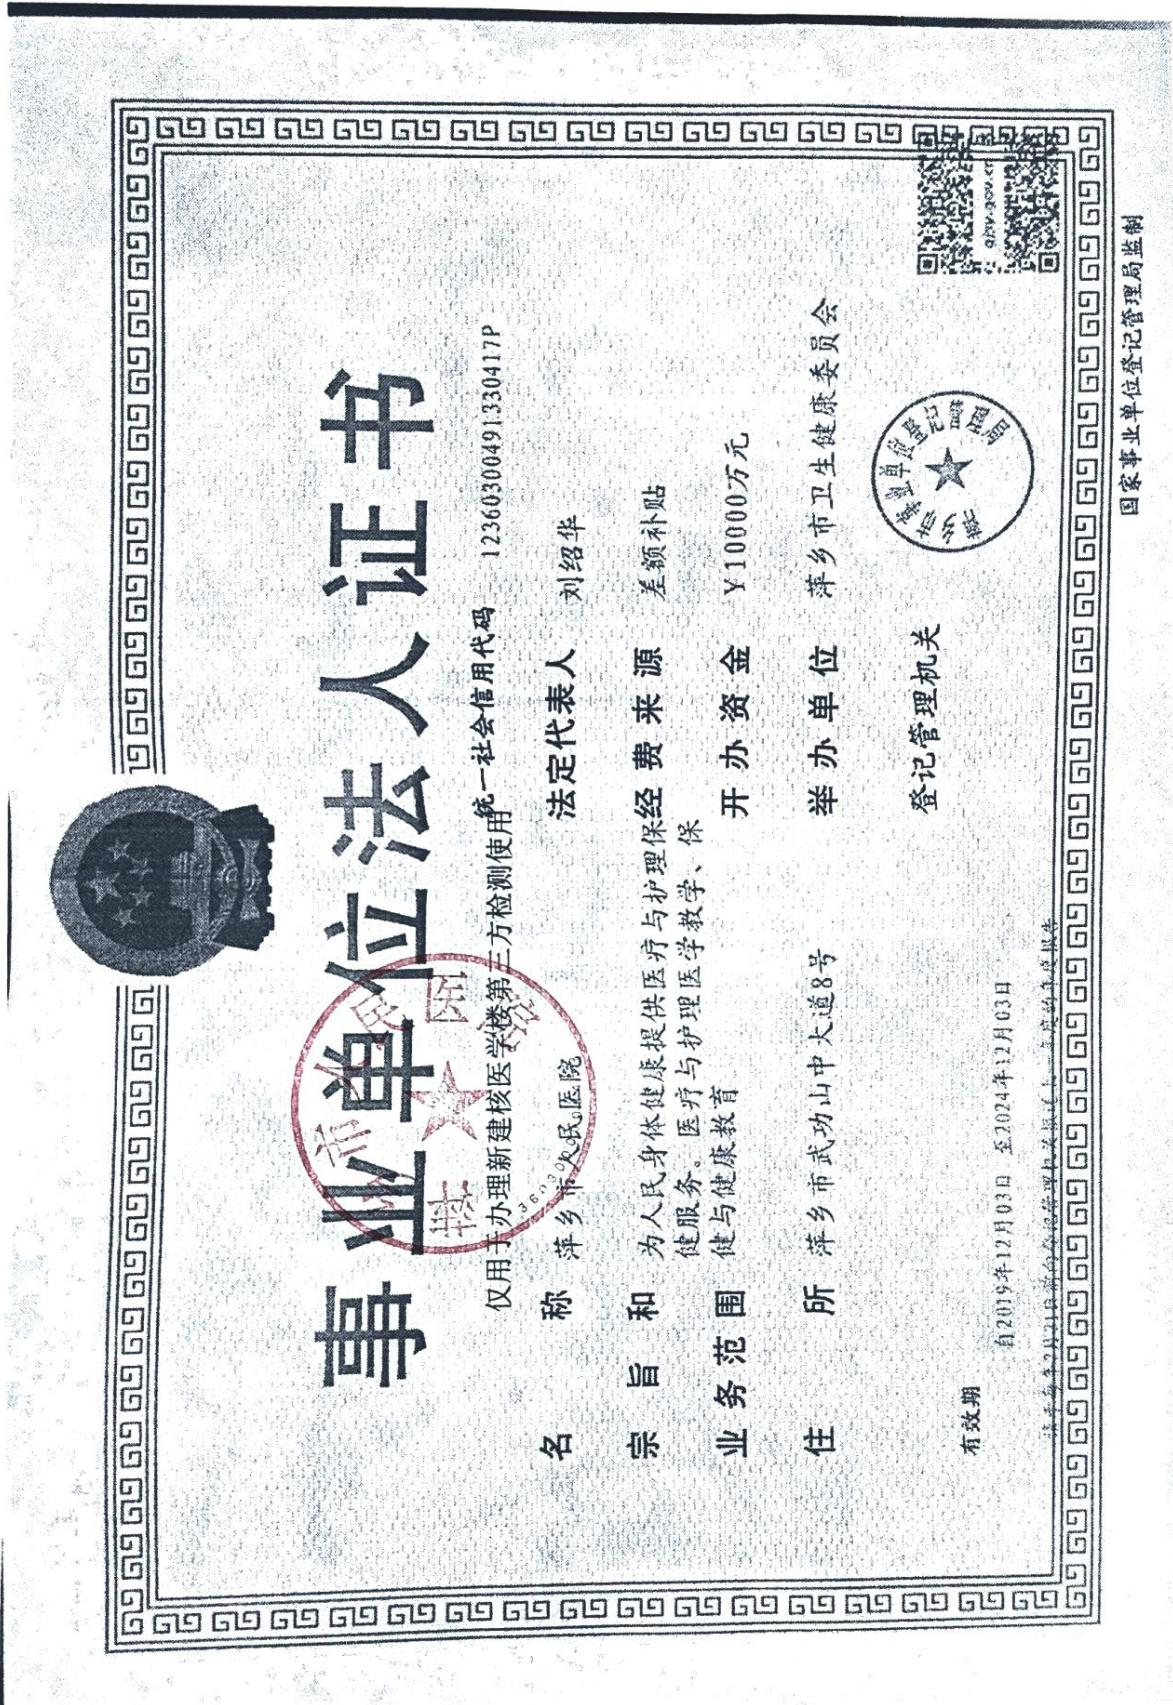
\includegraphics[width=0.85\linewidth]{images/58b34e5ac0d0bac8cefb1250fe27d42587f067fc5cb2431b060078f0aa9bfb60.jpg}
\end{figure}


\subsection{《医疗机构执业许可证》}

\begin{figure}[H]
\centering
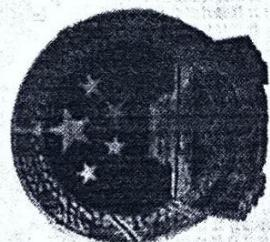
\includegraphics[width=0.85\linewidth]{images/848aa09e236011c3b078e8abac475b0fc7d1181e449e10ae64fb6fd704bf52f4.jpg}
\end{figure}


\begin{figure}[H]
\centering
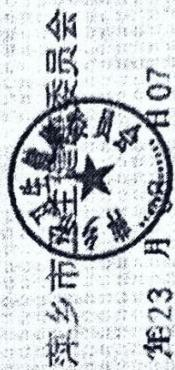
\includegraphics[width=0.85\linewidth]{images/8ae0b7dc8a7654a77fadce74d388f8aa507e284c1e3372b7751e8f3faabdf10f.jpg}
\end{figure}


\subsubsection{放射诊疗许可证}

赣卫放证字（2008）第004号

医疗机构名称萍乡市人民医院

负责人刘绍华

地 址萍乡市武功山中大道8号

许可项目放射治疗、核医学*

校验记录：

发证机关（盖章）

2023年09月

\begin{figure}[H]
\centering

\includegraphics[width=0.85\linewidth]{images/85eb07e986c89f19b759c75dfcc3d64bf44b46b410b918660fb294f263c2aafa.jpg}
\end{figure}

附件2-3 《放射诊疗许可证》

（许可范围见副本）

江西省卫生健康委员会制

扫描全能王

3亿人都在用的扫App

\subsubsection{放射诊疗许可证}

放证字（ 26第 号004

医疗机构名称：

负责人：

地 址：

许可项目：

校验记录：

萍乡市人民医院

刘绍华

萍乡市武功山中大道8号

放射治疗、核医学

\begin{figure}[H]
\centering
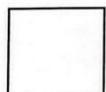
\includegraphics[width=0.85\linewidth]{images/f6b4a8abcaefa99fbcf5c4afc5edf64a514a23ff8174b1eac7c83f146b173bb5.jpg}
\end{figure}


\begin{figure}[H]
\centering
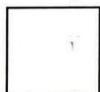
\includegraphics[width=0.85\linewidth]{images/6a943c1478d85a41994cf62c9d83816433841b7ca3597663b90a54319c344769.jpg}
\end{figure}


\begin{figure}[H]
\centering
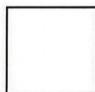
\includegraphics[width=0.85\linewidth]{images/45be4998cef9490eddc25be2b09f51ff54c8e70577a0c2bf7a57bf8707472244.jpg}
\end{figure}


\begin{figure}[H]
\centering
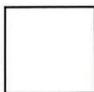
\includegraphics[width=0.85\linewidth]{images/9928778f726ba507e023195bcc9fbbac1625dcbcc3c8e31855fcab9509db8bfe.jpg}
\end{figure}


发证机关

海23

\begin{figure}[H]
\centering
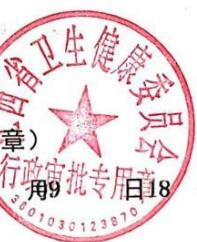
\includegraphics[width=0.85\linewidth]{images/4951ecf50dadfad07cb240a440d5a4f927345e2aef63f7f7b2470eb18778004a.jpg}
\end{figure}


第3页

S扫描全能王

放射诊疗许可范围
第4页

\begin{table}[H]
\centering
\begin{tabular}{|c|c|c|c|c|c|c|}
\hline
诊疗项目 & 项目明细 & 有或无 & 校验日期 &  &  &  \\
\hline
第一次 & 第二次 & 第三次 & 第四 &  &  &  \\
\hline
放射治疗 & 立体定向（Y刀、X刀）治疗 & 无 &  &  &  &  \\
\hline
医用加速器治疗 & 有 &  &  &  &  &  \\
\hline
质子等重粒子治疗 & 无 &  &  &  &  &  \\
\hline
钴-60机治疗 & 无 &  &  &  &  &  \\
\hline
后装治疗 & 有 &  &  &  &  &  \\
\hline
深部X射线机治疗 & 无 &  &  &  &  &  \\
\hline
敷贴治疗 & 无 &  &  &  &  &  \\
\hline
其他放射治疗项目 & 有 &  &  &  &  &  \\
\hline
核医学 & PET影像诊断 & 无 &  &  &  &  \\
\hline
SPECT影像诊断 & 有 &  &  &  &  &  \\
\hline
Y相机影像诊断 & 无 &  &  &  &  &  \\
\hline
\end{tabular}
\end{table}


\begin{figure}[H]
\centering

\includegraphics[width=0.85\linewidth]{images/0fa8c10d335d09d582b1121b492ba9cdd4663b539bbbd6e3149b123093f6295e.jpg}
\end{figure}


扫描全能王

3亿人都在用的扫报App

放射诊疗许可范围 (续表)
第5页

\begin{table}[H]
\centering
\begin{tabular}{|c|c|c|c|c|c|c|}
\hline
I & 项目明细 & 有或无 & 校验日期 &  &  &  \\
\hline
第一次 & 第二次 & 第三次 & 第四次 &  &  &  \\
\hline
 & 骨密度测量 & 无 &  &  &  &  \\
\hline
籽粒插植治疗 & 无 &  &  &  &  &  \\
\hline
放射性药物治疗 & 有 &  &  &  &  &  \\
\hline
其他核医学诊疗项目 & 无 &  &  &  &  &  \\
\hline
学 & DSA介入放射诊疗 & 无 &  &  &  &  \\
\hline
其他影像设备介入放射诊疗 & 无 &  &  &  &  &  \\
\hline
 & X射线CT影像诊断 & 无 &  &  &  &  \\
\hline
CR、DR影像诊断 & 无 &  &  &  &  &  \\
\hline
牙科X射线影像诊断 & 无 &  &  &  &  &  \\
\hline
乳腺X射线影像诊断 & 无 &  &  &  &  &  \\
\hline
普通X射线机影像诊断 & 无 &  &  &  &  &  \\
\hline
其它X射线影像诊断 & 无 &  &  &  &  &  \\
\hline
\end{tabular}
\end{table}


\begin{figure}[H]
\centering

\includegraphics[width=0.85\linewidth]{images/4327a55ea265a0d953a4c39978bbb8716a49fc0f7a20eecdb27aee912da0da82.jpg}
\end{figure}


扫描全能王

医用射线装置、放射性同位素概况
第6页

\begin{table}[H]
\centering
\begin{tabular}{|c|c|c|c|c|}
\hline
射线装置 & 类别 & 总台数 &  &  \\
\hline
II & 2 &  &  &  \\
\hline
III & 3 &  &  &  \\
\hline
 &  &  &  &  \\
\hline
非密封型放射性同位素 & 最大等效日操作量1.24x10\textasciitilde{}9Bq最大等效年操作量1.49x10 12Bq &  &  &  \\
\hline
工作场所级别个数 甲级 乙级 丙级 &  &  &  &  \\
\hline
密封型放射性同位素 & 密封源 & 核素 & 总数(个) & 总活度(Bq) \\
\hline
1r-192 & 1 & 3.7x10 11 &  &  \\
\hline
 &  &  &  &  \\
\hline
 &  &  &  &  \\
\hline
含密封源装置 & 装置名称 & 台数 & 总活度(Bq) &  \\
\hline
 &  &  &  &  \\
\hline
 &  &  &  &  \\
\hline
 &  &  &  &  \\
\hline
\end{tabular}
\end{table}


\begin{figure}[H]
\centering

\includegraphics[width=0.85\linewidth]{images/ccc6e32d65440fa68e62e42d199bdeb1b8de4c6cfc79e99d86f462dea45c79d7.jpg}
\end{figure}


扫描全能王

3亿人都在用的扫报App

射线装置明细

\begin{table}[H]
\centering
\begin{tabular}{|c|c|c|c|c|c|c|c|c|c|}
\hline
序号 & 装置名称 & 型号 & 生产厂家 & 设备编号 & 主要参数 & 所在场所 & 经办人及日期 & 变更情况 &  \\
\hline
变更事项 & 经办人及日期 &  &  &  &  &  &  &  &  \\
\hline
 & 1 直线加速器 & BJ-6B & 北京医疗研究所 & AE141 & X线 6Mv & 放疗室 & 李玉兰、杨智民2008年8月13日李玉兰、杨智民2008年8月13日熊燕、王志武2016年8月23 & 注销 & 胡芳2023.9.18 \\
\hline
 & 2 模拟定位机 & SL-I & 山东新华 & 181 & 120KV 500mA & 放疗室 &  &  &  \\
\hline
 & 3 SPECT/CT & INFIN IA HAWKE YE4GP & GE公司 & 18581 & 140KV 250mA & 核医学科(SPEC T室) & 胡青2023.9.18 &  &  \\
\hline
3 第7页 日 &  &  &  &  &  &  &  &  &  \\
\hline
\end{tabular}
\end{table}


\begin{figure}[H]
\centering

\includegraphics[width=0.85\linewidth]{images/94826bd128a6d9d23021d2def07c7837aafc6b3e73aea73d40c24314f2c1a060.jpg}
\end{figure}


扫描全能王

非密封型放射性同位素明细

\begin{table}[H]
\centering
\begin{tabular}{|c|c|c|c|c|c|c|c|c|}
\hline
核素 & 用途 & 物理状态 & 最大等效日操作量(Bq) & 最大等效年操作量(Bq) & 操作场所 & 经办人及日期 & 变更情况 &  \\
\hline
变更事项 & 经办人及日期 &  &  &  &  &  &  &  \\
\hline
I-131 & 诊断和治疗 & 液态 & 1.85x10\textasciicircum{}8 & 3.7x10\textasciicircum{}1 & 1核医学科1号分装室 & 熊燕、王志武2016年8月23日 &  &  \\
\hline
Tc-99 & 诊断 & 液态 & 7.4x10\textasciicircum{}8 & 1.11x10\textasciicircum{}12 & 核医学科2号分装室 & 熊燕、王志武2016年8月23日 &  &  \\
\hline
Sr-89 & 治疗 & 液态 & 2.74x10\textasciicircum{}8 & 1.37x10\textasciicircum{}10 & 核医学科注射室 & 熊燕、王志武2016年8月23日 &  &  \\
\hline
Sm-153-EDTMP & 治疗 & 液态 & 3.7x10\textasciicircum{}7 & 7.4x10\textasciicircum{}8 & 核医学科注射室 & 熊燕、王志武2016年8月23日 &  &  \\
\hline
\end{tabular}
\end{table}


第8页

\begin{figure}[H]
\centering

\includegraphics[width=0.85\linewidth]{images/ef6a802119fdaa512ac4456836ee78709b753c6ce52436e4fb11fc51d2552726.jpg}
\end{figure}


扫描全能王

3亿人都在用的扫报App

射线装置明细

\begin{table}[H]
\centering
\begin{tabular}{|c|c|c|c|c|c|c|c|c|c|}
\hline
序号 & 装置名称 & 型号 & 生产厂家 & 设备编号 & 主要参数 & 所在场所 & 经办人及日期 & 变更情况 &  \\
\hline
变更事项 & 经办人及日期 &  &  &  &  &  &  &  &  \\
\hline
4医速 & 用直线加TR 器GY & ILO Varian Co. & 621 & 8 X线 6Mv 放电1楼 电子线 6MeV、9MeV、12MeV、15MeV、18MeV、22MeV & 疗楼 高邓晓2018年10月15日 &  &  &  &  \\
\hline
\end{tabular}
\end{table}


第7页

\begin{figure}[H]
\centering

\includegraphics[width=0.85\linewidth]{images/2d503d8d51efd1cca52d845aa3ee4f548de985cc29758408d7dbc1f1b1a4bfad.jpg}
\end{figure}


扫描全能王

射线装置明细

\begin{table}[H]
\centering
\begin{tabular}{|c|c|c|c|c|c|c|c|c|c|}
\hline
序号 & 装置名称 & 型号 & 生产厂家 & 设备编号 & 主要参数 & 所在场所 & 经办人及日期 & 变更情况 &  \\
\hline
变更事项 & 经办人及日期 &  &  &  &  &  &  &  &  \\
\hline
5 放射治疗模 拟定位机 & Simul Simul n & Nucletro ML & 136 12 & OKV & 眼科楼 & 高锦辉 &  &  &  \\
\hline
ixEvo n & B.V. 11 & 160 50 & 0mA & 1楼 & 邓晓 &  &  &  &  \\
\hline
lntio n &  &  &  &  & 2018年10月15日 &  &  &  &  \\
\hline
\end{tabular}
\end{table}


第7页

\begin{figure}[H]
\centering

\includegraphics[width=0.85\linewidth]{images/a3b2186795a19f399b46b934f5af5e3bf531857debb2a20c8f65adfc8555ddcc.jpg}
\end{figure}


扫描全能王

3亿人都在用的扫报App

密封型放射性同位素明细

\begin{table}[H]
\centering
\begin{tabular}{|c|c|c|c|c|c|c|c|}
\hline
核素 & 活度(Bq) & 活度测量日期 & 生产厂家 & 所在场所 & 经办人及日期 & 变更情况 &  \\
\hline
变更事项 & 经办人及日期 &  &  &  &  &  &  \\
\hline
Ir-192 & 6.33x10\textasciicircum{}10 & 2016年6月 & 北京原子高科 & 放疗室 & 熊燕、王志武2016年8月23日 & 活度变更3.7X10\textasciicircum{}11场所变更为放疗楼1楼 & 高锦辉 邓晓 2016年10月15日 \\
\hline
\end{tabular}
\end{table}


第9页

\begin{figure}[H]
\centering

\includegraphics[width=0.85\linewidth]{images/63c65779685be2145adb563608997b49ff04cba8a31538667d20afbf099f7774.jpg}
\end{figure}


扫描全能王

含密封源装置明细
第10页

\begin{table}[H]
\centering
\begin{tabular}{|c|c|c|c|c|c|c|c|c|c|c|}
\hline
编号 & 装置名称 & 型号 & 生产厂家 & 放射源 & 所在场所 & 经办人及日期 & 变更情况 &  &  &  \\
\hline
核素 & 活度(Bq) & 活度测量日期 & 变更事项 & 经办人及日期 &  &  &  &  &  &  \\
\hline
1 & 高剂量率γ射线遥控后装治疗机 & HDR18B & 山东新华医疗器械股份有限公司 & Ir-192 & 3.7×10\textasciicircum{}11 & 2018.7 & 放疗室 & 熊燕、王志武2016年8月23日 & 场所变更为放疗楼;活度变更为3.7×10\textasciicircum{}11 & 高锦辉邓晓2018年10月15日 \\
\hline
\end{tabular}
\end{table}


\begin{table}[H]
\centering
\begin{tabular}{|c|c|c|c|c|c|c|c|c|c|}
\hline
序号 & 装置 名称 & 型号 & 生产厂家 & 设备 编号 & 主要 参数 & 所在 场所 & 经办 人及 日期 & 变更情况 &  \\
\hline
变更 事项 & 经办 人及 日期 &  &  &  &  &  &  &  &  \\
\hline
1 2 3 4 5 6 7 & 血管造影X线 系统（大C） 血管造影X线 系统（大C） CT机 CT机 CT机 DRBuck DR Essenta DRcompact & ALLURA XerF P20 Innova 4100-38 Brilliance Hispeed dual DISCOVER CT750HD Digital Diagnost Egitaly Diagnost Digital Egitaly Digital Digital Digital Digital Digital Digital Digital Digital Digital Digital Digital Digital Digital Digital Digital Digital Digital Digital Digital Digital Digital Digital Digital Digital Digital Digital Digital Digital Digital Digital Digital Digital Digital Digital Digital Digital Digital Digital Digital Digital Digital Digital Digital Digital Digital Digital Digital Digital Digital Digital \#\# & 荷兰 美国GE讯 美国 北京航工 美国 美国GE公司 北京浦河 系统 飞利浦司 飞利浦2可 飞利浦2可 & 1518 654708 6384 158100HMS 441625 CN1 120kV 500mA 11000061 & 140kV 1200mA 125kV 1000mA 140kV 500mA 140kV 835mA 6600008 602017 120kV 500mA & \#入科 \#入科 \#入科 \#入科 \#入科 \#入科 \#入科 \#入科 &  &  &  \\
\hline
\end{tabular}
\end{table}


\begin{table}[H]
\centering
\begin{tabular}{|c|c|c|c|c|c|c|c|c|c|}
\hline
序号 & 装置名称 & 型号 & 生产厂家 & 设备编号 & 主要参数 & 所在场所 & 经办人及日期 & 变更情况 &  \\
\hline
变更事项 & 经办人及日期 &  &  &  &  &  &  &  &  \\
\hline
891011234567891011121345678910112134567891011213456789101121345678910112134567891011213456789101121345678910112134567891011213456 &  &  &  &  &  &  &  &  &  \\
\hline
\end{tabular}
\end{table}


\begin{table}[H]
\centering
\begin{tabular}{|c|c|c|c|c|c|c|c|c|c|}
\hline
序号 & 装置名称 & 型号 & 生产厂家 & 设备编号 & 主要参数 & 所在场所 & 经办人及日期 & 变更情况 &  \\
\hline
变更事项 & 经办人及日期 &  &  &  &  &  &  &  &  \\
\hline
17 & 床边X光机 & MobiletMira & 德国西门8 & 10378 & 133kV 450mA &  & 吴洁清 2017.9 & 注销 & 吴洁琼 \\
\hline
18 & 骨密度测量仪 & Excepu & 美国诺兰德 & 2028 & 100kV 13mA &  &  &  &  \\
\hline
19 & 心脏X射线机 & KodakZ100Multimc & 美国 Ca restream & B3GA05 & 40-70kV 42/10mA &  &  &  &  \\
\hline
20 & 床边X光机 & DISCOVER & Hologic公司 & 89080 & 40-70kV 13-60mA 160kV 14.3m &  &  &  &  \\
\hline
21 & 骨密度测量仪 & optimaCT540 & 舒止通电气压系统有限公司 & CBLCG 3000029 HM & 140kV 400mA &  &  &  &  \\
\hline
\end{tabular}
\end{table}


\begin{table}[H]
\centering
\begin{tabular}{|c|c|c|c|c|c|c|c|c|c|}
\hline
序号 & 装置名称 & 型号 & 生产厂家 & 设备编号 & 主要参数 & 所在场所 & 经办人及日期 & 变更情况 &  \\
\hline
变更事项 & 经办人及日期 &  &  &  &  &  &  &  &  \\
\hline
23 & 口腔CT CT(62排) 全景X射线机 & PP3 Optim aCT62 0 Planmeca ProMax & 思瑞德斯有限责任公司 航卫通用电气医疗系统有限公司 Planmeca Oy & BCZG2 10002 OHM prpr2 50522 & 90ky 16mA 140k V 560mA 84KV 16mA & 医疗综合大楼影像科 230室 医疗综合楼二楼影像科 医疗综合楼五楼口腔科 & 2020.5.25. &  &  \\
\hline
\end{tabular}
\end{table}


\begin{table}[H]
\centering
\begin{tabular}{|c|c|c|c|c|c|c|c|c|c|}
\hline
序号 & 装置名称 & 型号 & 生产厂家 & 设备编号 & 主要参数 & 所在场所 & 经办人及日期 & 变更情况 &  \\
\hline
变更事项 & 经办人及日期 &  &  &  &  &  &  &  &  \\
\hline
26 & 口腔X射线机 口腔CT & Kodak 2100 PP3 & Carestream Health, Inc. 思瑞德斯有限责任公司 & YGXBO 24 SE190 2228 & 40-7 0KV 4-10 mA 99kV 16mA & 医疗综合楼五口腔科 医疗综合楼五楼口腔科 & 2023 1.16 &  &  \\
\hline
\end{tabular}
\end{table}


\begin{table}[H]
\centering
\begin{tabular}{|c|c|c|c|c|c|c|c|c|c|}
\hline
序号 & 装置名称 & 型号 & 生产厂家 & 设备编号 & 主要参数 & 所在场所 & 经办人及日期 & 变更情况 &  \\
\hline
变更事项 & 经办人及日期 &  &  &  &  &  &  &  &  \\
\hline
28 & 全数字化乳腺X射线机CT(32排) & SeleniaDimensionsSOMATOMgo. UP & 豪洛捷公司上海西门子医疗器械有限公司 & GAN170100468108790 & 39kV200mA130kV400mA & 健康管理中心二楼健康管理中心二楼CT室 &  &  &  \\
\hline
\end{tabular}
\end{table}


\begin{table}[H]
\centering
\begin{tabular}{|c|c|c|c|c|c|c|c|c|}
\hline
射线装置明细 &  &  &  &  &  &  &  &  \\
\hline
装置名称 & 型号 & 生产厂家 & 设备编号 & 主要参数 & 所在场所 & 经办人及日期 & 变更情况 &  \\
\hline
变更事项 & 经办人姓名 &  &  &  &  &  &  &  \\
\hline
DR & Multix Fusion Max 翔 龙 Max & 上海西门子医疗器械有限公司 & 40340 & 150kV 1000mA & 健康管理中心二楼204DR室 &  &  &  \\
\hline
T(256排) & SOMATO M Force & 上海西门子医疗器械有限公司 & 76824 & 140kV 1000mA & 医疗综合楼二楼影像科 &  &  &  \\
\hline
CT & SOMATO M Confidence & 上海西门子医疗器械有限公司 & 100558 & 140kV 666mA & 医疗综合楼二楼介入科复合手术室 &  &  &  \\
\hline
DSA & ARTIS Pheo & 上海西门子医疗器械有限公司 & 164782 & 125kV 1000mA & 医疗综合楼二楼介入科复合手术室 &  &  &  \\
\hline
DSA & Azuric n 7 Mzo & 上海西门子医疗器械有限公司 & 2109 & 125kV 1000mA & 医疗综合楼二楼介入科 DSA-1 &  &  &  \\
\hline
C形臂 & OEC one CFD & 北京通用电气华伦医疗设备公司 & BB9SS2200 160HL & 110KV 20mA & 医疗综合楼四楼手术室 &  &  &  \\
\hline
\end{tabular}
\end{table}


\begin{table}[H]
\centering
\begin{tabular}{|c|c|c|c|c|c|c|c|c|c|}
\hline
序号 & 装置名称 & 型号 & 生产厂家 & 设备编号 & 主要参数 & 所在场所 & 经办人及日期 & 变更情况 &  \\
\hline
变更事项 & 经办人及日期 &  &  &  &  &  &  &  &  \\
\hline
36 & X射线探测和体层摄影设备 & SOMATOgOSin & 上海西门子医疗器械有限公司 & 129116 & 140KV825mH & 敖杉街长孔路下桥 & 2025.3.18无字清理 &  &  \\
\hline
 &  &  &  &  &  &  &  &  &  \\
\hline
\end{tabular}
\end{table}


\section{本项目辐射源项}

\begin{table}[H]
\centering
\begin{tabular}{|c|c|c|c|c|c|c|c|c|c|c|}
\hline
序号 & 装置名称 & 生产厂商 & 型号 & 主要参数 & 拟安装场所 & 来源 & 源分类 &  &  &  \\
\hline
含源装置 & 放射源 &  &  &  &  &  &  &  &  &  \\
\hline
1 & 后装治疗机 & 待定 & 待定 & 最大装载活度 & 3.7×10\textasciicircum{}11Bq(10Ci) & 源类型 & 192Ir & 肿瘤大楼一楼后装治疗机房 & 拟新购 & III类 \\
\hline
物理状态 & 固体 &  &  &  &  &  &  &  &  &  \\
\hline
半衰期 & 74.0d &  &  &  &  &  &  &  &  &  \\
\hline
平均能量 & 0.37MeV (γ) &  &  &  &  &  &  &  &  &  \\
\hline
周围剂量当量率常数（裸源） & 0.111μSv·m²/MBq·h &  &  &  &  &  &  &  &  &  \\
\hline
\end{tabular}
\end{table}


\begin{table}[H]
\centering
\begin{tabular}{|c|c|c|c|c|c|c|c|c|}
\hline
序号 & 设备 & 预期诊疗患者人次 & 单人次平均出 束时间 & 周工作天数 & 年工作周数 & 周工作量 (h) & 年工作量 (h) & 备注 \\
\hline
1 & 后装治疗机 & 6人次/天 & 10min & 5 & 50 & 5.0 & 250 & 设备质控时间约10分钟/ 次/周 \\
\hline
注：年最大工作量=预期日诊疗患者人次/台×单人次出束时间×周工作天数×年工作周数 &  &  &  &  &  &  &  &  \\
\hline
\end{tabular}
\end{table}


\section{放射防护设计方案}

放射治疗项目机房屏蔽设计情况表

\begin{table}[H]
\centering
\begin{tabular}{|c|c|c|c|}
\hline
机房名称 & 屏蔽体 & 屏蔽设计材料及厚度 &  \\
\hline
后装治疗机房 & 东墙 & 屏蔽体厚度 & 800mm 混凝土 \\
\hline
北墙 & 迷路内墙厚度 & 800mm 混凝土 &  \\
\hline
迷路外墙厚度 & 800mm 混凝土 &  &  \\
\hline
西墙 & 屏蔽体厚度 & 800mm 混凝土 &  \\
\hline
南墙 & 屏蔽体厚度 & 800mm 混凝土 &  \\
\hline
顶盖 & 屏蔽体厚度 & 800mm 混凝土 &  \\
\hline
地坪 & /(注:下方土层) &  &  \\
\hline
防护门 & 屏蔽厚度:10.0mmPb 类型:电动推拉门 &  &  \\
\hline
机房 & 位置 & 单位(mm) &  \\
\hline
后装治疗机 & 源离各墙的距离 & ≥1.0m &  \\
\hline
\end{tabular}
\end{table}


\begin{figure}[H]
\centering
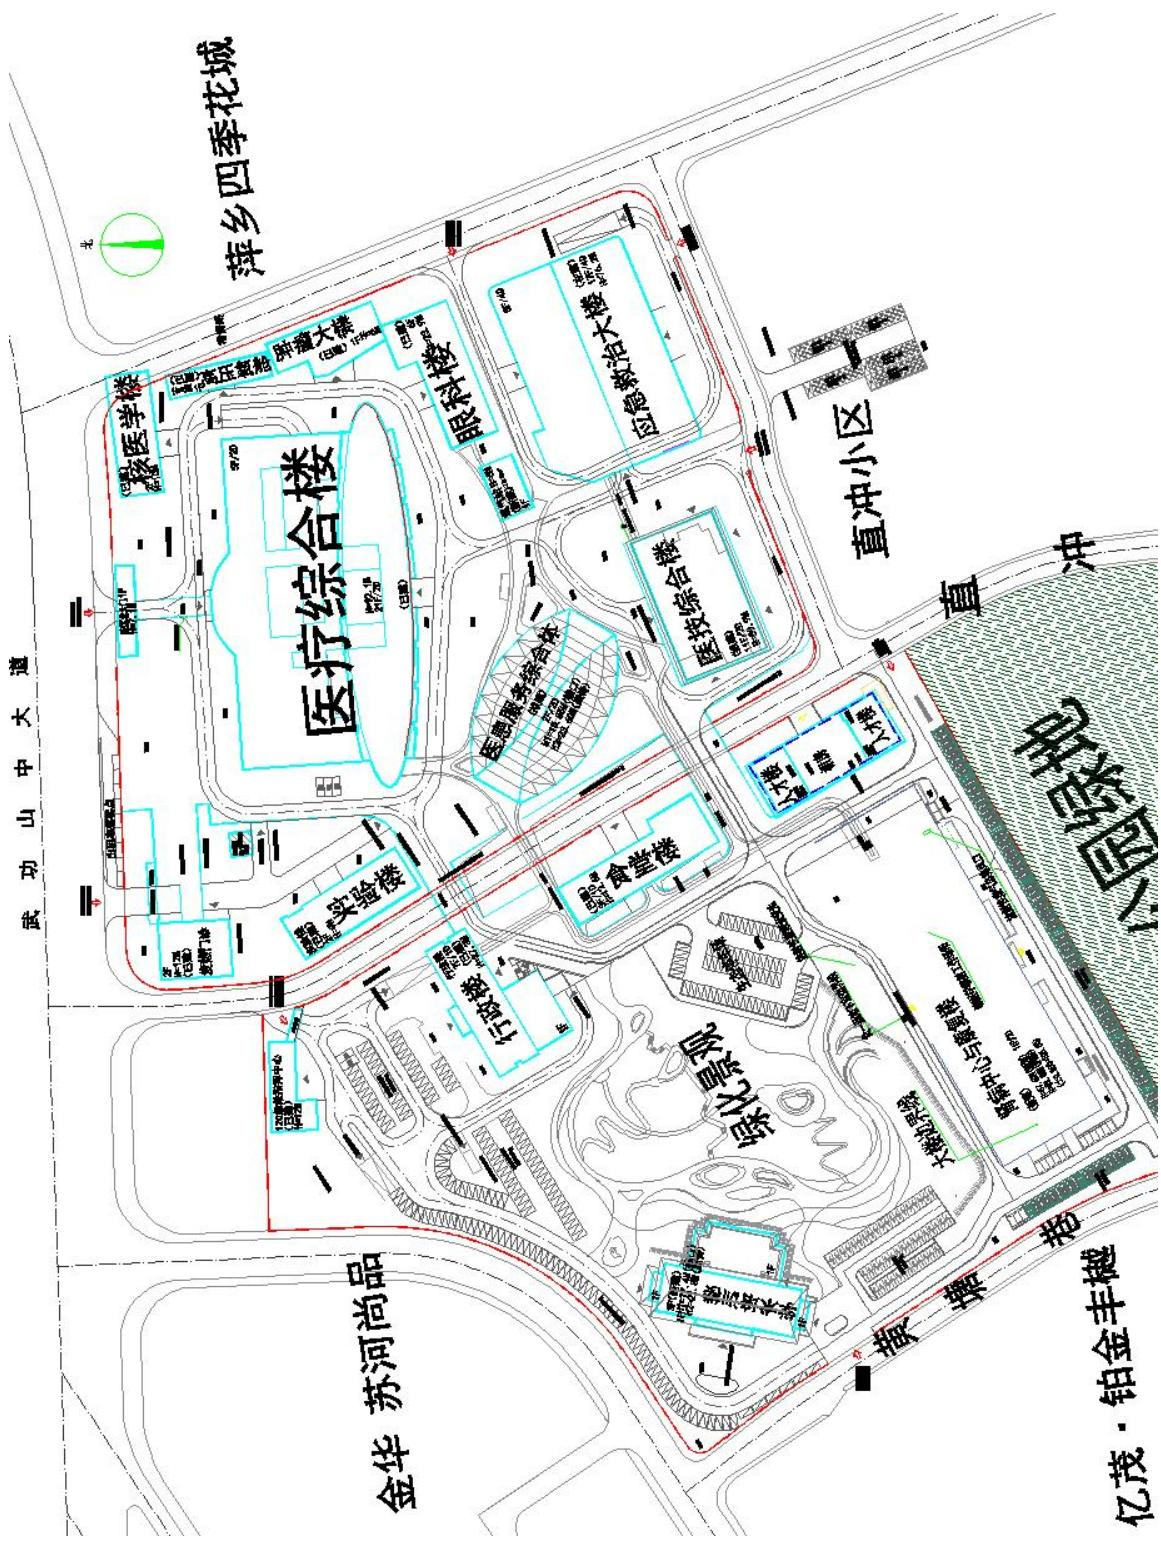
\includegraphics[width=0.85\linewidth]{images/b0eff78e095665f7bb5339e7178b8f2370b57cc78ad07d6dff12a7bb9fdc5f60.jpg}
\end{figure}

附件5 本项目相关图纸

\begin{figure}[H]
\centering
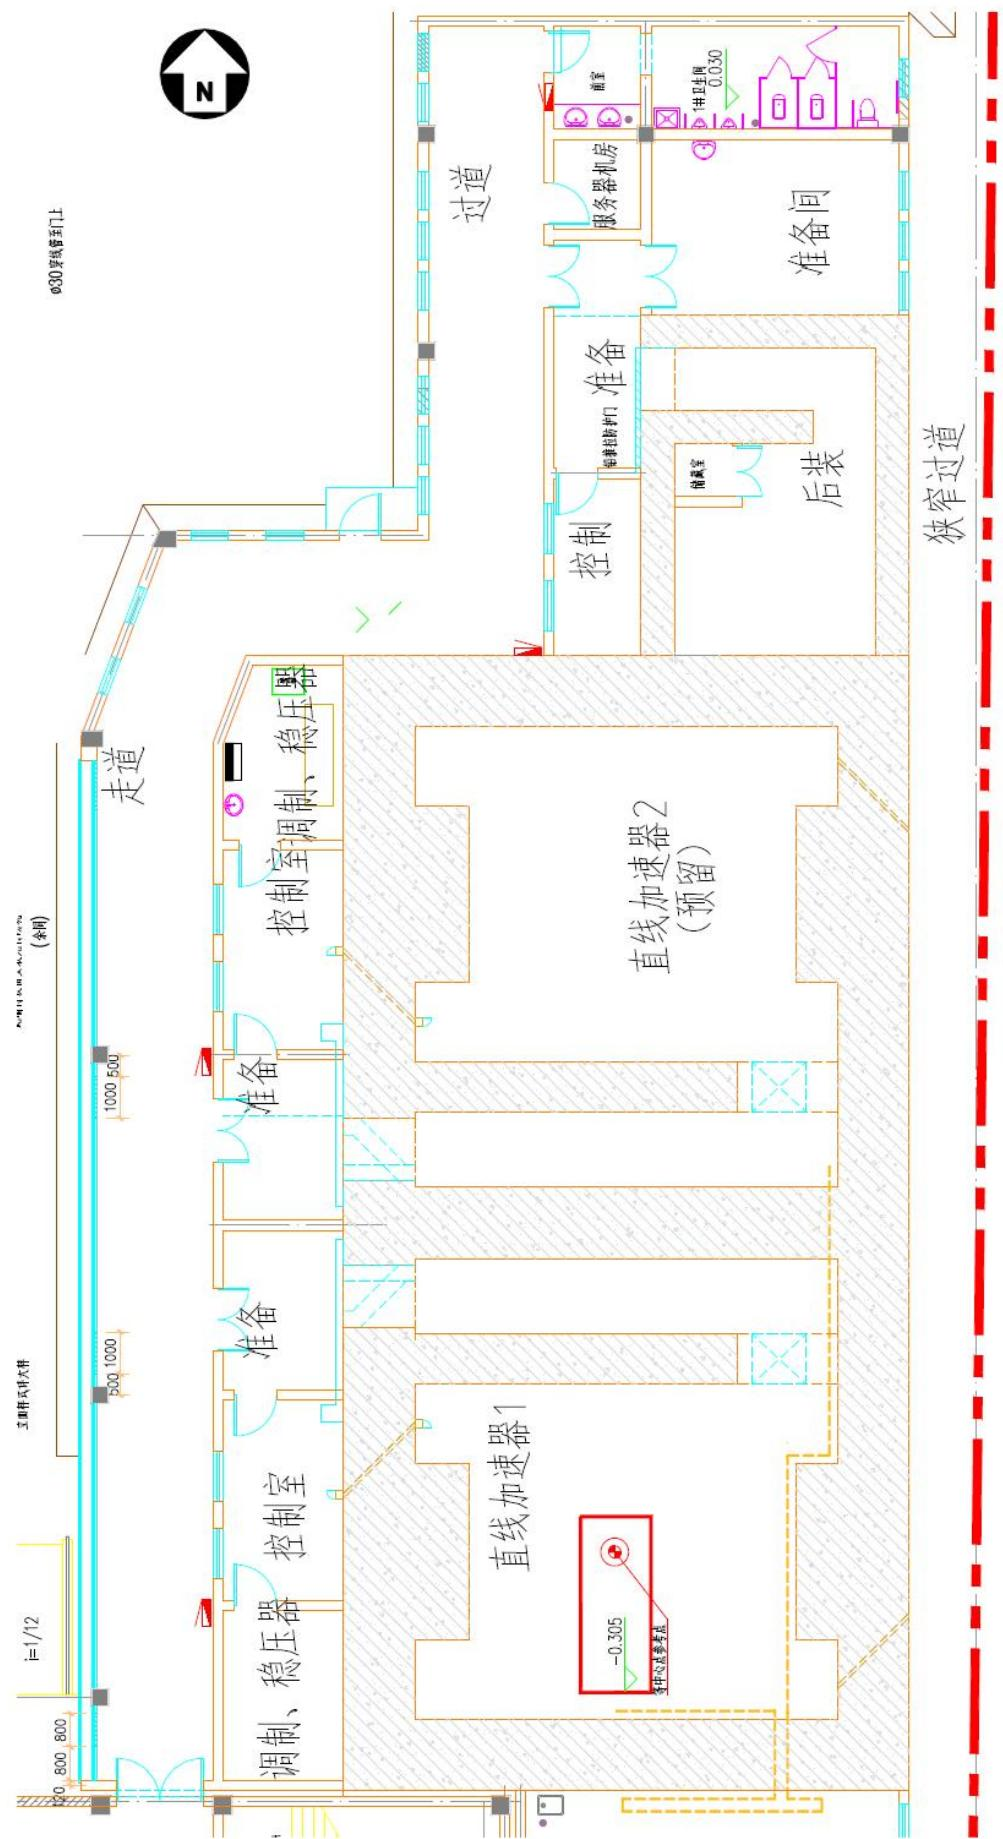
\includegraphics[width=0.85\linewidth]{images/f170078922a389aa86dc2e49f791b1d513c199c3928cde1496a2375925be5e88.jpg}
\end{figure}


\section{放射防护管理组织制度}

\subsubsection{萍乡市人民医院临床管理部}

\subsubsection{关于成立辐射安全与放射防护管理机构的通知}

各科室：

为强化医院辐射安全与放射防护管理工作，保证医疗质量和医疗安全，保障放射工作人员、患者和公众的健康，根据国家相关规定，我院决定成立辐射安全与放射防护管理机构，现将有关决定通知如下：

\subsubsection{一、管理机构人员组成：}

组长：刘绍华

第一副组长：何建中

副组长：郑志刚

组员：易飞、潘朝阳、邹南安、黄文军、张雨虹、汤江林、董文哲、李丰章、邓四海、王俊东、胡芯源、黄勇全、李莺、王爱华、文毅强、黄飞、陈佳龙

郑志刚同志为我院辐射防护负责人。

辐射安全与防护管理机构办公室设在公共卫生科。办公室主任由公共卫生科陈佳龙同志作为专职人员担任；兼职人员由公共卫生科廖光辉负责日常监督工作。

\subsubsection{二、管理机构主要职责：}

1、认真贯彻执行国家相关规定，接受各级生态环境部门、卫生健康行政部门和公安部门等有关部门的监督与检查；
2、制定和监督实施我院的各项辐射安全与放射防护工作制度，展开安全防护政策、安全知识和安全技术教育；
3、制定我医院辐射事故应急预案，负责辐射事故应急预案的日常演练和辐射事故处置；
4、每年定期召开涉放射项目专题工作会议，研究部署解决放射诊疗和核技术利用工作中存在的重大问题；
5、定期安排辐射安全与放射防护专项检查，消除各种辐射安全与放射防护隐患；
6、安排相关技术人员对设备进行维护保养，定期检查本医院放射工作人员的技术操作情况，定期检查辐射安全与放射防护措施及设备是否存在防护漏洞，以保证工作人员、患者及公众的安全性：
7、做好工作人员的辐射安全与放射防护培训、防护设施及个人防护用品的供应与管理以及辐射安全与放射防护档案与个人健康档案的建立与管理等工作。

\subsubsection{三、各成员职责}

\subsubsection{组长职责：}

组长负责宏观管理，对重大问题做出决策，对整个医院的安全及辐射事故负责。

\subsubsection{副组长职责：}

副组长负责具体的管理工作，首先做到思想重视，不断宣传辐射安全与放射防护的方针政策，对辐射安全与放射防护工作要定期研究、布置、检查、制定规章制度、及时解决和处理防护工作中的重大问题和事故。组织审查和批准新、改、扩建项目的辐射安全与放射防护措施及辐射事故管理等。

\subsubsection{管理员职责：}

专职和兼职管理员负责处理日常具体业务：

\begin{enumerate}
\item 负责办理放射诊疗许可和辐射安全工作，放射诊疗项目和核技术利用项目取得各种相关许可证后方能投入使用；
\item 负责建立放射诊疗项目和核技术利用项目相关管理工作档案并及时更新。
\item 负责放射工作人员个人剂量的定期检测，有异常情况报告主管领导；
\item 负责放射诊疗项目和核技术利用项目中各射线装置操作规程的执行监督工作；
\item 负责定期进行安全联锁系统等辐射安全与放射防护设施及措施的检查，出现问题及时报告领导并解决；
\item 负责对全体放射工作人员进行辐射安全与放射防护教育，确保不出现辐射事故；
\item 认真接受卫生健康行政部门及生态环境部门对本单位辐射安全与放射防护工作的检查及对设备的监测、工作场所的监测评价，并做好整改工作；
\item 负责自主监测仪器和设备的正常运行及年度检定工作；
\item 负责放射工作人员的职业健康管理及档案的建立；
\item 负责辐射安全与放射防护档案的建立及管理。
\end{enumerate}

\begin{figure}[H]
\centering
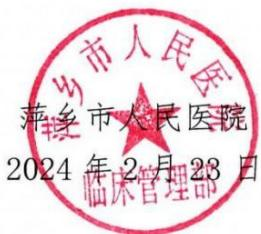
\includegraphics[width=0.85\linewidth]{images/575f0979a6d33f0b2b9db8edae5520a0162baf8fbb00da63c98d1aafd9384c62.jpg}
\end{figure}


\section{应急预案}

\subsubsection{萍乡市人民医院临床管理部}

\subsubsection{萍乡市人民医院辐射事故应急预案}

\subsubsection{一、总则}

依据《中华人民共和国职业病防治法》《放射诊疗管理规定》《放射性同位素与射线装置安全和防护条例》等相关法律、法规规定，强化应对突发放射事故的应急处置能力，提高医院职工对放射事故应急防范的意识，最大限度地保障放射工作人员与受检者及公众的安全，做到对放射事故早发现，速报告，快处理，建立快速反应机制，特制定本预案。

应急原则：以人为本，预防为主。

\subsubsection{二、应急组织及职责：}

医院成立辐射事故应急处理领导小组，组织成员名单如

组长：郑志刚

副组长：陈佳龙

委员：易飞、潘朝阳、邹南安、黄文军、张雨虹、汤江林、龚敏、韩涛、赖丹、王稻、任妹、刘书娜、陈军、董文哲、李丰章、邓四海、王俊东、胡芯源、黄勇全、李莺、王爱华、文毅强、黄飞

\subsubsection{应急救援办公室：0799-6881712}

主要职责：

\begin{enumerate}
\item 负责组织应急准备工作，调度人员，指挥类职能人员迅速赶赴现场，首先采取措施保护工作人员和公众的生命安全，保护环境不受污染，最大限度控制事态发展；
\item 对辐射事故的现场进行组织协调，安排救助，不让无关人员进入，保护好现场，指挥辐射事故应急救援行动；
\item 迅速、正确判断事件性质，负责向上级行政主管部
\end{enumerate}

门报告辐射危害事件应急救援情况；

\begin{enumerate}
\item 负责恢复本单位正常秩序。稳定受照人员情绪等方面的工作。
\end{enumerate}

\subsubsection{二、事件报告和应急响应：}

发生辐射事故后，事故单位应当立即启动本单位的辐射事故应急响应，采取必要措施，并在2小时内填写《辐射事故初始报告表》，向当地生态环境部门、卫生健康行政部门报告。造成或可能造成人员辐射损伤照射的，还应同时向当地卫生健康部门报告。

1、立即终止原放射活动，切断继续泄露可能；封锁现场，迅速撤离有关人员，对事故受照射人员进行及时检查、救治和医学观察实行现场警戒，划定紧急隔离区，保护好事故现场。
2、发现辐射事故的第一发现人要立即逐级上报，科室在接到事故报告后要初步判断事故类型，并在接到报告30分钟内上报到公共卫生科、设备科、医务科及保卫科。现场处置人员应根据辐射事故的不同类型特点，配备相应的专业防护装备，采取安全防护措施，严格按照应急人员出入事发现场的程序执行，控制应急响应人员的辐射剂量，保护应急响应人员的人身安全。
3、接到辐射事故报告后，立即上报医院主管院长，同时组织相关科室进行应急处理并在事故发生两小时内上报萍乡市生态环境局（市生态环境局24小时值班电话：6778203）、萍乡市卫健委（医政处电话：6879191）、市公安局电话：110。
4、人体受超剂量照射事故时，接到报告后的医院主管部门应当迅速安排受照射人员接受医学检查或者在指定的医疗机构救治，同时积极配合上级相关主管部门的调查。
5、接到事故报告后，要立即组织有关人员赶赴事故现

场，并配合上级管理机关的调查。

6、事故发生2小时内，按《辐射事故初始报告表》填写书面报告报送市生态环境局、市卫健委。
7、发生辐射事故的射线装置和场所修复后，现场监测合格，经生态环境主管部门、卫生健康行政部门批准后，辐射事故应急预案尚可解除。

\subsubsection{三、辐射事故等级划分}

根据辐射事故的性质、严重程度、可控性和影响范围等因素，从重到轻将辐射事故分为特别重大辐射事故、重大辐射事故、较大辐射事故和一般辐射事故四个等级。

特别重大辐射事故，是指I类、I类放射源丢失、被盗、失控造成大范围严重辐射污染后果，或者放射性同位素和射线装置失控导致3人以上（含3人）急性死亡。

重大辐射事故，是指I类、I类放射源丢失、被盗、失控，或者放射性同位素和射线装置失控导致2人以下（含2人）急性死亡或者10人以上（含10人)急性重度放射病、局部器官残疾。

较大辐射事故，是指类放射源丢失、被盗、失控，或者放射性同位素和射线装置失控导致9人以下（含9人）急性重度放射病、局部器官残疾。

一般辐射事故，是指IV类、V类放射源丢失、被盗、失控，或者放射性同位素和射线装置失控导致人员受到超过年剂量限值的照射。

\subsubsection{四、应急准备}

为了保证辐射事故应急工作的有效进行，辐射事故防治工作领导小组要做好事故应急的人员、物资的准备工作，主要包括以下内容：

1、辐射事故应急工作的基本任务是减少危害、保护公众、保护环境。

2、有关科室要做好辐射事故应急准备和应急响应的详细方案。
3、准备必要的应急设施、设备和相互之间快速可靠的通讯联路系统。
4、准备辐射监测系统、防护器材、药械和其他物资，用于辅助事故应急工作的设施、设备和通讯联络系统，辐射监测系统以及防护器材、药械等，应当处于良好状态。
5、定期对职工进行辐射安全与放射防护事故应急知识的专门培训；对辐射事故应急工作人员进行培训，适时组织进行放射事故应急演练。

\subsubsection{五、培训和演练}

\section{培训}

应急预案和应急计划确立后，按计划对全体人员进行放射安全事件及放射治疗事故应急处理的培训（培训的内容应包含： $\textcircled{1}$辐射安全与放射防护基本知识和相关法规、标准，$\textcircled{2}$可能发生的辐射事故及其医学应急处理措施， $\textcircled{3}$所涉及的应急预案或程序， $\textcircled{4}$急救基本知识和操作技能等），每年培训一次，培训后由科室组织考核。

\section{演练}

每年组织一次应急预案演练，提高应急指挥水平和应急救援能力，并根据培训和演练情况修改完善应急方案。本方案自文件印发之日起施行。

\begin{figure}[H]
\centering
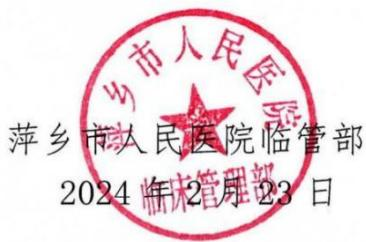
\includegraphics[width=0.85\linewidth]{images/6134a3e36e7fda1900ff43f9c2336af519e6b3d5dd843c655eacc62fa39cf640.jpg}
\end{figure}


\section{放射防护管理制度}

放射治疗质量管理制度

\subsubsection{放射治疗质量管理制度}

\subsubsection{一、目的：}

为了规范科室实施放射治疗的流程，保障患者获得正确的治疗方案和高质量的放射治疗，制定本制度。

\subsubsection{二、建立规范的病历档案}

患者入院后，按照肿瘤患者的特殊病历书写要求，建立患者病历档案，首先记录患者临床症状的发生时间、伴随症状和发展规律，既往诊疗医院和诊疗过程，有无病理诊断，每次治疗的详细方案，目前病情变化和一般情况等。其次根据患者入院后需要完善实验室检查和影像学检查资料，明确病理诊断，全面准确的评估病情，确定临床诊断及分期，如果入院前患者相关检查资料及诊断已经基本完成，可以直接完成病历书写，最好是24小时内完成病历的建立，完善必要的检查后为下一步治疗方案的讨论做好准备。

\subsubsection{三、讨论制定治疗方案}

患者实施放疗之前，应由主治医师以上资格的医师组织进行该患者治疗方案的集体讨论，讨论人员包括管床住院医师、主治医师、其他相关专业的会诊医师。根据患者的临床特点、病理诊断、临床或病理分期、治疗经过、一般状况和经济能力等，按照综合治疗和个体化治疗的原则，讨论患者整体治疗策略、是否实施放疗、有无放疗禁忌症等内容，最后形成统一的治疗

意见，并告知患者或者患者家属，签署知情同意书。

\subsubsection{四、放疗体位固定和模拟定位}

经过临床医生的讨论决定实施放射治疗后，根据不同的放射治疗部位选择适当的放射治疗技术。放射治疗有二维常规照射、后装内照射、3DCRT、IMRT、IGRT、SGRT、SBRT、SRS(SRT)等多种技术模式,根据需要分别在X线定位机、CT-sim、MRI-sim和PET-CT下进行

放射治疗质量管理制度

影像学定位，放射治疗师根据不同的技术模式和定位方式选择体位固定材料和固定方式并完成放疗模拟定位。

\subsubsection{五、放射治疗的靶区讨论}

在精确放射治疗模式中，患者的定位扫描影像数据经过初步处理后，应由具备放射治疗上岗证的主治医师以上资格的医师负责治疗靶区的讨论和勾画，经与物理师讨论后勾画出放疗靶区和需要保护的重要器官组织轮廓图。放射治疗靶区包括GTV(CT、MRI等显示的肿瘤轮廓);CTV(包括GTV和肿瘤可能侵犯的亚临床病灶)：PTV(考虑了患者器官运动和摆位误差的CTV).

\subsubsection{六、计划设计和评估优化}

勾画完成放射治疗靶区和重要保护器官组织轮廓后，物理师按照临床医师设定的参数条件利用放射治疗计划系统设计照射方式和参数，设计完成后与临床医师反复讨论评估，利用DVH曲线和剂量曲线图等多种方式评价计划优劣，最终确定最优的放疗计划。评估优化的目标是在保证肿瘤获得足够放疗剂量的同时，尽可能控制重要器官组织的照射剂量不超过其耐受剂量，从而保护重要器官组织的功能和患者生活质量

\subsubsection{七、放射治疗计划的验证}

放射疗计划执行之前，由临床医师和放射治疗师进行治疗中心位置验证，射野验证，放射物理师做三维剂量验证。治疗中心位验证是依照计划系统给出的肿瘤中心位置，找出对应的体表标志作为放疗摆位时的依据。射野验证是指在确定治疗中心位置后，利用直线加速器使用电子射野验证系统或CBCT扫描肿瘤中心图像与TPS图像配准。剂量验证是由物理师核实体内所接受的射线照射剂量与计划系统所设计的照射剂量是否一致。 民医院

\subsubsection{八、治疗计划的实施}

治疗计划验证后由经管医生带领病人和治疗计划到直线加速器治疗室实施放射治疗。病人第

放射治疗质量管理制度

一次治疗时放射治疗师必须校队患者姓名、放疗编号，在治疗中心利用EPID或CBCT对计划进行实时野验证，配准误差由经管医生签字确认后对患者实施治疗。调强放疗病人治疗前三次每天一次CBCT验证，在治疗阶段的过程中每周至少一次CBCT验证。

\subsubsection{九、放射治疗计划的记录保存}

整个放射治疗工作是由临床医生、放射物理师和肿瘤放射治疗师协作完成，放射治疗计划也是保证患者放射治疗顺利实施的具体规划，必须在放射治疗计划执行当天详细记录入病历当中，并随病历存入病历档案中。放射治疗计划单是患者执行高质量放射治疗的书面依据和过程记录，同时因为治疗单涉及患者隐私，必须在治疗过程中和治疗后妥善保存，不得随意交与

患者或者其他非本科室人员。

\subsubsection{放射治疗装置维护、维修制度}

一、严格遵守国家颁布的各项法律法规，严格执行相关部门和生产厂家制定的维护维修程序、在科主任的领导和技术组长的管理下，按照有关职能部门指导，开展对放射治疗装置维护维修工作。
二、认真做好放射治疗装置的定期维护保养工作。定期检查放射治疗装置工作电压、波导气压、内循环水压参数并及时加以纠正。检查各种机械运动是否正常及环境温度、湿度等情况，做到出现问题及时处理。
三、保证放射治疗装置的各种安全连锁功能工作可靠，必须及时排除任何安全隐患，防止事故发生，确保患者和工作人员安全。
四、严格按照生产厂家的要求对放射治疗装置开展维修工作。协助配合设备维保单位尽力尽快排除故障，满足临床治疗。要做好维修记录，分析并向上级报告。确保放射治疗装置安全可靠运行。
五、维修完毕通知物理质控人员，对相关参数进行测量校准，对放射治疗装置进行质量控制和管理。
六、协助做好安全防护宣教和监测工作。配合做好放射治疗装置的年度检查等工作。

\subsubsection{放射工作人员职业健康管理制度}

为了保障放射工作人员的健康利益，依据《中华人民共和国职业病防治法》《放射诊疗管理规定》《放射工作人员职业健康管理办法》等法律法规的规定，制定放射工作人员职业健康管理制度

一、放射工作人员是我院放射工作人员包括从事放射诊疗活动受到电离辐射照射的人员。
二、放射工作人员应当具备下列条件：

1.年满18周岁。
2.经职业健康检查，符合放射工作人员的职业健康要求。
3.放射防护和有关法律知识培训考核合格。
4.遵守放射防护法规和规章制度，接受职业健康监护和个人剂量监测管理。

\subsubsection{三、基本要求}

为每位放射工作人员建立放射防护管理档案；不安排未成年人从事接触电离辐射危害的工作：不安排未经上岗前职业健康检查的人员从事接触电离辐射危害的工作：不安排孕期、乳期从事对本人和胎儿、婴儿接触电离辐射危害的工作；不安排有电离辐射职业禁忌证的职工从事所接触电离辐射危害的工作。不安排未经上岗前放射防护培训的人员从事接触电离辐射危害的工作

\subsubsection{四、放射工作人员上岗前的管理}

1.放射工作人员上岗前接受卫生健康行政部门放射防护法规和防护知识培训考核和辐射安全与防护考核，均合格后方可参加相应的放射工作。
2.对新分配和调入的放射岗位的人员按《放射工作人员健康要求及监护规范》规定的体检项目进行上岗前的职业性健康体检，根据卫生技术服务机构的体检结果，如可从事放射工作，方可从事放射工作。
3.上岗时纳入个人剂量监测管理，放射工作人员佩戴了个人剂量后方可从事放射工作。

\subsubsection{五、放射工作人员在岗期间的管理}

1.每2年按《放射工作人员健康要求及监护规范》规定的体检项目进行在岗期间的职业性健康体检。若发生异常，调查、分析原因、必要时进行健康检查。在收到职业健康检查报告的7日内，如实告知放射工作健康检查中发现不宜继续从事放射工作的人员，应当及时调离放射工作岗位，并妥善安置；对需要复查和医学随访观察的放射工作人员，应当及时予以安排。通过职业性健康体检发现疑似和确诊为职业性放射病的，立即报告卫生健康行政部门和社会保障部门，并妥善处置疑似或确诊的职业性放射病病人，职工接受职业健康检查期间按正常出勤

\subsubsection{放射工作人员个人剂量管理制度}

一、按照《放射工作人员职业健康管理办法》和国家有关标准、规范的要求，安排本单位的放射工作人员接受个人剂量监测，并遵守以下规定：

\begin{enumerate}
\item 外照射个人剂量监测周期不超过3个月，内照射个人剂量监测周期按照有关标准执行。
\item 建立并保存个人剂量监测档案。
\item 允许放射工作人员查阅、复印本人的个人剂量监测档案。
\end{enumerate}

\subsubsection{二、个人剂量监测档案主要内容}

1.常规监测方法和结果等相关资料。
2.应急或者事故中受到照射的剂量和调查报告等相关资料。放射工作单位应当将个人剂量监测结果及时做好记录。

\subsubsection{三、放射工作人员进入放射工作场所，应当遵守以下规定：}

1.正确佩戴个人剂量计。根据工作状态正确佩戴个人剂量牌，并妥善保管个人剂量牌。对于辐射主要来自前方时（如诊断放射学工作人员）个人剂量牌佩戴在人体躯干前方中部位置，一般在左胸前或锁骨对应的领口位置。对于介入放射学、核医学放射药物分装与注射等全身受照不均匀的工作情况，采用双剂量计监测方法，一个佩戴在铅围裙外锁骨对应的领口位置，另外一个佩戴在铅围裙内躯干上。严禁将内外剂量牌混淆佩戴，如出现此情况，需及时告知负责人。
2.离岗时将个人剂量牌及时交给科室负责人，严禁中途更换佩戴者。
3.工作人员工作时，应将个人剂量计随身佩戴，禁止将个人剂量计遗弃在机房内，由此造成个人剂量计检测结果超标，造成影响和后果的，本人负全责。必要时，调离工作岗位。
四、个人剂量监测工作应当由具备资质的个人剂量监测技术服务机构承担，并按照规定，将报告送达放射工作单位。
五、当收到个人剂量监测机构对于周期内有放射工作人员的职业受照剂量大于调查水平的情况核查表时，当事人和科室负责人需进行调查分析，如实告知是否出现过以下情况（个人剂量计曾经被打开、个人剂量计曾经被水浸泡、个人剂量计曾经被留置于放射工作场所内、曾经佩戴个人剂量计接受过放射性检查、曾经佩戴个人剂量计扶持接受放射性检查的受检者/患者、曾经维修含源装置、铅围裙内外剂量计混淆佩戴；如果是正常佩戴，是否发以下情况：佩戴期间工作量较前期明显增加、其他原因），如为真实时需进行进步调查分析。

处理。对参加应急处理或者受到事故照射的放射工作人员，及时组织健康检查或者医疗救治，按照国家有关标准进行医学随访观察。

2.每2年组织放射工作人员参加放射防护和法律法规有关知识培训，培训考核，每5年参加一次生态环境部门组织的辐射安全防护考核，考核合格后方可再次从事辐射安全工作。
3.每季度将放射工作人员佩戴的个人剂量计送交委托的个人剂量监测机构进行剂量监测。若发生异常，调查、分析原因、告知本人并采取相应措施，必要时进行健康检查。

\subsubsection{四、放射工作人员离岗时的管理}

职工退休或者其他原因和本单位解除合同时，必须进行职业性健康检查，并将职工本人的健康监护档案复印交给本人，其健康监护档案原件按管理规定的保存年限进行保存。

\subsubsection{六、放射工作人员档案管理}

1.按要求为放射工作人员建立职业健康监护管理档案。
2.保存培训档案。培训档案应当包括每次培训的课程名称、培训时间、考试或考核成绩等资料。
3.终身保存个人剂量监测档案。保存内容：个人剂量监测结果、异常情况处理分析情况、应急或者事故中受到照射的剂量和调查报告等相关资料
4.终身保存职业健康体检档案。保存内容：职业史、既往病史和职业照射接触史；历次职业健康检查结果及评价处理意见；职业性放射性疾病诊疗、医学随访观察等健康资料。
5.放射工作人员可查阅、复印本人的职业健康监护档案。放射工作单位应当如实、无偿提供

\subsubsection{七、津贴、休假及疗养}

1.承担本单位放射工作人员职业健康检查、职业性放射性疾病的诊断、鉴定、医疗救治和医学随访观察的费用。
2.放射工作人员的保健津贴按照国家要求发放，并在国家统一规定的休假外，放射工作人员每年可以享受放射保健休假 $2 \sim 4$周（科室根据从事放射工作满10年的在岗放射工作人员，定时组织参加相关

\begin{figure}[H]
\centering
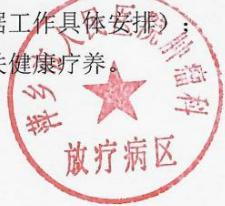
\includegraphics[width=0.85\linewidth]{images/7ff563f77a176410b187fdacffd77a9dbe7557e9be79a60e715d0ffeff156644.jpg}
\end{figure}


\subsubsection{放疗医师岗位职责}

\subsubsection{资质认定条件：}

1.1具有大学医学本科或以上学历；
1.2持有《医师执业证书》，并符合执业地点、执业类别与执业范围的要求；
1.3.持有《大型医用设备上岗合格证》；
1.4.持有《放射人员工作证》和《辐射安全与防护培训合格证书》；
1.5经过一年以上的放疗专业培训。

\subsubsection{放射治疗住院医师技术能力要求：}

2.1.对病员进行检查、诊断、治疗，开写医嘱并检查其执行情况。
2.2书写病历。新入院病员的病历，一般应在病员入院后8小时内完成首次病程录，24小时内完成入院记录。检查和改正实习医师的病历记录。并负责病员住院期间的病程记录，及时完成病员的出院小结。
2.3向主治医师及时报告诊断、治疗上的困难以及病员病情的变化，提出需要转科或出院的意见。
2.4在上级医师指导下，学习放射治疗患者定位、治疗计划制定、放射治疗过程中的处理、放射治疗后随访。

\subsubsection{放射治疗主治医师技术能力要求：}

3.1.主持病区的临床病例讨论及会诊，检查、修改下级医师书写的医疗文件，决定病员出院，审签出(转)院病历。
3.2.组织本组医师学习与运用国内外先进医学科学技术，开展新技术、新疗法，进行科研工作，做好资料积累，及时总结经验。
3.3.担任临床教学，指导进修、实习医师工作。
3.4.能参与各种肿瘤普通放射治疗技术，及精确放射治疗技术(三维适形放射治疗、调强放射治疗、影像引导下的放射治疗和立体定向放射治疗)的患者定位，治疗计划制定，但

放疗计划需经(副)主任医师审核方可实施。

4放射治疗（副)主任医师技术能力要求：

4.1定期查房并亲自参加指导急、重、疑、难病例的抢救处理与特殊疑难和死亡病例的讨论会诊。
4.2指导本科主治医师和住院医师做好各项医疗工作，有计划地开展基本功训练。
4.3担任教学和进修、实习人员的培训工作。
4.4定期参加门诊工作。
4.5.能独立完成各种常见肿瘤及各种少见病、疑难病例的普通放射治疗技术，及精确放射治疗技术(三维适形放射治疗、调强放射治疗、影像引导下的放射治疗和立体定向放射治疗)的患者定位，治疗计划制定，放射治疗过程中的处理。
4.6各级医师每年均需通过放疗科个人业务能力考核。

\subsubsection{放疗技师职责}

1.准确、熟练地使用放疗机器，了解机器的结构和工作原理，以及常规操作的重要性，严格按操作规程使用机器，发生故障及时向维修人员汇报。
2.摆位治疗中，能解决一些疑难患者的摆位，并协助物理师检查治疗计划，核对射线能量、照射剂量、射野结构以及楔形板的使用是否正确。
3.合理安排患者的治疗时间，对于重症患者实行优先治疗原则。
4.治疗前了解患者病情，介绍放疗相关注意事项，耐心解答患者的疑虑，消除其恐惧心理
5.治疗中严格坚守岗位，密切注意患者治疗状况，有特殊情况及时处理并作好记录。
6.认真填写治疗单，经常核对剂量有无差错，治疗单字迹工整、清晰、准确，治疗完后签字确认。每周至少核对一次治疗单剂量，发现问题及时更正，如有较大差错应及时报告主任。
7.参与放射治疗质量控制，积极持续改进
8.协助相关部门做好放疗设备的维护保养、维修等工作。
9.了解国内外放疗技术的新进展和动态，积极配合有关人员开展放疗新课题的研究。
10.治疗工作结束后，检查机器及辅助设备、门窗、水、电关闭情况及安全、卫生情况。

\subsubsection{放疗物理师职责}

1.参加并通过全国物理师上岗证资格考试，获得物理师上岗证。
2.有较好的外语和计算机基础，对解剖学、放射生物学、核医学和影像诊断有一定的了解。
3.通晓所有放疗设备的原理及各类射线的物理特点，能协助医生针对临床具体情况选择机型并按放疗原则确定放疗方案。
4.了解并掌握各类辐射测量手段，主要是电离室、热释光、半导体、胶片计量学方法，在新设备安装验收后按规程准确刻度剂量及用三维水箱或体模测量各种必要的临床数据，能借助人形体模或患者自身实测临床剂量。
5.熟悉治疗计划系统的操作，能指导或协助各类技术人员工作，并建立和完善特殊治疗技术和计量学方法。
6.与医生一起建立并不断完善临床计量学步骤，使患者治疗前的全部准备工作和实施过程有条不紊，各环节配合默契。
7.不断关注放疗设备和技术的发展，不断更新知识层次和知识面，开展新治疗技术，在购置新设备后着手开展临床和剂量方面的科研和教学工作。
8.负责放疗技术的QA、QC工作，和治疗机及放射工作人员的辐射防护事宜。

\subsubsection{放疗科维修人员岗位职责}

1.在科主任领导下，负责放疗设备的安装、调试和维修工作。
2.判定各种放疗设备的安全操作及规章制度并督促检查执行情况。
3.定期检查放疗设备的运转状态，发现问题及时处理，保证机器正常运行。
4.掌握国内外放疗设备发展情况，引进新技术，做好科研和教学工作，当好科主任的参谋。
5.协助技术组工作，负责检查督促福射安全防护工作。

\subsubsection{放射工作人员个人剂量管理制度}

一、按照《放射工作人员职业健康管理办法》和国家有关标准、规范的要求，安排本单位的放射工作人员接受个人剂量监测，并遵守以下规定：

\begin{enumerate}
\item 外照射个人剂量监测周期不超过3个月，内照射个人剂量监测周期按照有关标准执行。
\item 建立并保存个人剂量监测档案。
\item 允许放射工作人员查阅、复印本人的个人剂量监测档案。
\end{enumerate}

\subsubsection{二、个人剂量监测档案主要内容}

1.常规监测方法和结果等相关资料。

2.应急或者事故中受到照射的剂量和调查报告等相关资料。放射工作单位应当将个人剂量监测结果及时做好记录。

三、放射工作人员进入放射工作场所，应当遵守以下规定：

1.正确佩戴个人剂量计。根据工作状态正确佩戴个人剂量牌，并妥善保管个人剂量牌。对于辐射主要来自前方时（如诊断放射学工作人员）个人剂量牌佩戴在人体躯干前方中部位置，一般在左胸前或锁骨对应的领口位置。对于介入放射学工作，采用双剂量计监测方法，一个佩戴在铅围裙外锁骨对应的领口位置，另外一个佩戴在铅围裙内躯干上。严禁将内外剂量牌混淆佩戴，如出现此情况，需及时告知负责人。
2.离岗时将个人剂量牌及时交给科室负责人，严禁中途更换佩戴者。
3.工作人员工作时，应将个人剂量计随身佩戴，禁止将个人剂量计遗弃在机房内，由此造成个人剂量计检测结果超标，造成影响和后果的，本人负全责。必要时，调离工作岗位。
四、个人剂量监测工作应当由具备资质的个人剂量监测技术服务机构承担，并按照规定，将报告送达放射工作单位。
五、当收到个人剂量监测机构对于周期内有放射工作人员的职业受照剂量大于调查水平的情况核查表时，当事人和科室负责人需进行调查分析，如实告知是否出现过以下情况（个人剂量计曾经被打开、个人剂量计曾经被水浸泡、个人剂量计曾经被留置于放射工作场所内、曾经佩戴个人剂量计接受过放射性检查、曾经佩戴个人剂量计扶持接受放射性检查的受检者/患者、曾经维修含源装置、铅围裙内外剂量计混淆佩戴；如果是人民发正常佩戴，是否发生过以下情况：佩戴期间工作量较前期明显增加、其他原因)，如为真实时，需进行进一步调查分析。

\subsubsection{肿瘤科放疗室放射防护管理制度}

\subsubsection{一、安全管理员及其职责}

放疗病区应配备专（兼）职的管理人员，负责放射治疗工作的质量保证和安全防护。其主要职责是：

1.组织制定并落实放射治疗和放射防护管理制度；
2.定期组织对放射治疗工作场所、设备和人员进行放射防护检查；
3.组织本病区放射治疗工作人员接受专业技术放射防护知识及有关规定的培训和健康检查；
4.制定放射事件应急预案并组织演练；
5.记录本病区发生的放射事件并及时报告管理部门。

\subsubsection{二、放疗设备和仪表的检测要求}

1.新安装、维修和更换重要部件后的设备，应当经省级以上卫生行政部门资质认证的检测机构对其进行检测，合格后方可启用；
2.定期进行稳定性检测、校正和维护保养，由省级以上卫生行政部门资质认证的检测机构每年至少进行一次状态检测：
3.按照国家有关规定检验或校准用于放射防护和质量控制的检测仪表；
4.放射治疗设备及其相关设备的技术指标和安全防护性能，应当符合有关标准与要求；
5.不合格或国家有关部门规定淘汰的放射治疗设备不得购置、使用、转让和出租。

\subsubsection{三、安全防护装置}

放疗科放疗场所应配备并使用安全防护装置、辐射监测仪器和个人防护用品，具体为：设置民医院所多重安全连锁系统、剂量监测系统影像监控、对讲装置和固定式剂量监测报警装置、配备放疗剂量仪、剂量扫描装置和个人剂量报警仪。

\subsubsection{四、警示标识}

1.装有放射性同位素的设备和容器，应设有电离辐射标识，在放射性同位素储存场所，应设有电离辐射警告标识及必要的文字说明；
2.按规定将放射治疗场所分为控制区、监督区，在控制进出口及其他适当位置，设有电离辐射警告标识和工作指示灯。

\subsubsection{五、个人防护}

放疗室应对从业人员进行上岗前、在岗期间和离岗时的健康检查，定期进行专业及防护知识培训，分别建立个人剂量、职业健康管理和教育培训档案。从业人员应按规定佩戴个人剂量计。

\subsubsection{六、放射事件防范}

放疗室应当制定防范和处置放射事件应急预案；发生放射事件后应当立即采取应急救援和控制措施，防止事件的扩大和蔓延。当发生下列情形时，应当及时进行调查处理，如实记录，报告医院管理部门：

1.放射治疗实际照射剂量偏离处方剂量25\%以上的；
2.人员或射野误照；
3放射源丢失、被盗或污染的；
4.设备故障或人为失误引起的放射事件。

\subsubsection{放疗科患者须知}

\subsubsection{一、放射治疗中患者须知：}

1、每次治疗时，请尽量让自己的身体与定位时的状态保持一致，如：定位时如果要憋尿，治疗时也应如此。因为治疗体位与定位体位的一致对您治疗的准确性至关重要，如果技术员为您摆好的体位与定位时不同或使您感到不适，请及时与技术员沟通，做出调整。
2、保持身上红色标记线清晰，如脱落切不可自行描画，必须找主管医生重新标记。
3、请您按照每天的预约时间段到治疗室门前候诊厅等候，不要比预约时间来的过早，也不要迟到。有时因为安排新加病人治疗，可能会将您的治疗时间稍推后，这种情况无法避免，我们会尽力使您按时治疗，希望您谅解。
4、放疗期间，每周至少见主管医生一次，以便医生了解病情变化并及时对症处理。（医生每天十点前会在病房查房，门诊治疗的病人请在十点后在住院部放疗科诊室找医生。）如有不适可随时找医生处理。
5、患者请遵医嘱配合必要的辅助护理，如：妇科患者放疗期间需配合阴道冲洗，鼻咽、鼻腔及鼻窦肿瘤患者需配合鼻腔冲洗，口咽患者应按医嘱漱口。
6、对待放疗中的不适反应，不必过分紧张和焦虑，可告知医生，医生会及时作出相应处理，有些症状在放疗结束后2-4周内会逐渐好转或消失。较为严重者，需收入院。
7、照射区皮肤忌暴晒、搓洗，贴身衣服要柔软宽松，最好是棉质衣料，如有溃荡出现，切勿自行使用膏剂涂抹，不能包，要在放疗医生的指导下用药，
8、治疗期间应保持体重，如因消瘦或浮肿致模具过松或过紧，请告知医生，确认是否需要调整治疗计划。
9、您每天的治疗时间相对固定，如遇特殊情况，如停电、设备故障等我们

会及时用电话通知您。设备故障不可避免，但我们会尽快维修，所以当与此类情况时，请您耐心等待，保持电话畅通。

\subsubsection{二、放疗后患者须知：}

1、妇科患者放疗后遵医嘱需坚持3-6个月的阴道冲洗。
2、鼻咽、鼻腔及鼻窦患者放疗后遵医嘱坚持鼻腔冲洗及饭前饭后漱口，口咽患者坚持每天饭前饭后漱口3周至1月来我科复查，根据情况决定后续治疗安排。
3、皮肤反应明显的患者应保持患处通风、干燥，遵医嘱外用药物。
4、饮食方面等注意事项同放疗期间要求。
5、放疗后免疫力低下可行免疫治疗。
6、放疗后一般会发生放疗反应，有些反应是迟发性放疗后很长一段时间才会表现出来，有些反应如果能及时发现及时处理完全可以恢复，否则造成严重的后果将会影响患者的生存质量，因此患者务必对复查给以足够的重视。复查的时间一般可以在治疗后的3\textasciitilde{}6个月，有些情况可遵医嘱在治疗后1个月复查，以后每半年或1年复查一次。如有不适随时到我科复查。
7、我们会定期电话或信件随访，关注您的病情变化，请您积极配合我们的随访。如果您电话号码或通信地址变化，请您打电话告知我们，保证我们能够联系到您。

\subsubsection{后装治疗操作规程}

需要后装治疗的病人，到后装准备间，躺后装治疗床，先由医生按要求安放好施源器，并固定稳妥。
将患者推入CT定位机房，由后装治疗床转移到CT定位床，进行CT扫描。扫描结束后确认各施源器、插值针到达指定位置，如有不同。及时进行调整并重扫CT。
三．CT扫描结束后，将患者推送到后装准备间。CT图像传送到后装治疗计划系统。
四．1、在靶区勾画系统中进行正常组织器官勾画及靶区勾画。
2、按治疗计划步骤和医生对治疗计划的要求，作治疗计划及计划优化。
3、医生查看计划不符合要求时，应反复调整修改，直至医生满意，认可为止。
4、打印输出治疗计划。
5、物理师、医生在计划上签名存档备用。

五.把病人送入治疗室，将施源器与治疗机输出的相应端口一一连接，不能接错，各接头必须到位。

六治疗：

1、将计划提供的治疗参数输入治疗机。
2、查看治疗计划参数是否准确无误。
3、确认无误后批准计划，开始治疗。
4、治疗结束后，打印当次治疗日志，治疗操作者及医生必须在治疗单上签名存档备查。

由医师取下施源器，并进行相应处理。
八．安放、取下施源器时应严格无菌操作。
九．后装治疗为放射性同位素源，操作过程中，应尽量减少射线对人体的损害和环境污染。

\begin{figure}[H]
\centering
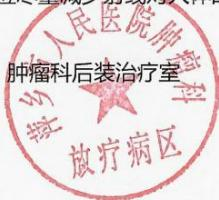
\includegraphics[width=0.85\linewidth]{images/77f2d4940beb678023d35ff317ef607793ee0beffb560312cc6553806a8211e0.jpg}
\end{figure}


\subsubsection{放射治疗核查制度}

一、各班技术员必须认真仔细阅读每一张治疗单，核对各种治疗条件（射线种类、能量、治疗方式、照射野、面积、机架角度、准直器角度等)，严格正确摆位，开机架再次核对治疗条件，确认无误后开机治疗。
二、由科内中级职称以上人员组成摆位抽查小组，每月一次对摆位作随机抽查，内容包括：治疗体位、所用附件、照射野面积、床升高度、照射野中心点是否吻合等，并作好记录。
三、技术组长，每月一次对各班摆位作随机抽查，并记录。
四、科主任，每月一次对特殊治疗病人的摆位作随机抽查，并记录。
五、每月底总结本周摆位抽查结果，指出不足，并交换个人的摆位质量做出评分。
六、每周一次对治疗单进行总查对， 及各种治疗条件是否正确无误，

和每一张治疗单的累计量是否正确。

\begin{figure}[H]
\centering
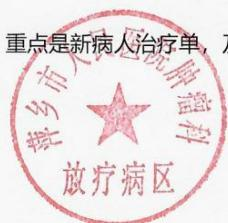
\includegraphics[width=0.85\linewidth]{images/17706125f0f1e40eadd32b90e44cec5f93c54940b19b29f74ad94a053161dbce.jpg}
\end{figure}


\subsubsection{放射治疗计划讨论制度}

\subsubsection{建立规范的病历档案}

按照肿瘤患者的特殊病历书写要求建立患者病历档案，完善完善实验室检查和影像学检查，

明确病理诊断，全面准确的评估病情，为下一步治疗方案的讨论做好准备。

\subsubsection{讨论制订治疗方案}

由主治医师以上资格的医师组织进行治疗方案的集体讨论，形成统一的治疗意见，告知患者

或家属签署知情同意。

\subsubsection{治疗部位的影像学定位}

定位之前由医师和放射治疗师根据治疗需要共同制作固定装置进行体位固定,在CT室进行

CT下模拟定位获取影响资料，并传输至TPS计划系统，由物理师进行初步的数据处理。

\subsubsection{放射治疗的靶区讨论}

由具备LA医师上岗证的主治以上资格的医师负责治疗靶区的讨论和确认，与物理师讨论后

勾画出放疗靶区和需要保护的重要器官。5、计划设计和评估优化

物理师按照医师的要求利用TPS计划系统设计治疗计划，医师利用DVH曲线等工具评价计

划，最终确定最优的治疗计划，目标是保证肿瘤获得足够放疗剂量的同时尽可能的保护正常

器官的功能以及患者的生活质量。

\subsubsection{放射治疗计划的验证}

计划执行之前，由物理师进行中心位置验证、射野验证和剂量验证，验证后方可执行。

\subsubsection{放射治疗计划的实施及记录保存}

计划实施当天详细记录入病历，并随病历存入病历档案中。记录单涉及患者隐私需妥善保管，

不得丢失或泄露。

\subsubsection{放射源管理制度}

1、放射源辐射防护符合国家电离辐射防护与辐射源安全基本标准。
2、在购置新源时，应与放射源生产单位(或原出口国或废源集中贮存设施)签订废弃放射源贮存和处置协议。新购放射源必须有国家统一编号。
3、新建、扩建、改建的放射源建设项目，必须经环保部门验收合格后方可使用。
4、、配备必要的检查或监测设备。受辐射剂量较高的技术和操作维修人员要配备带报警装置的个人辐射剂量计。
5、对运行中含放射源的装置和场所，要配置剂量监测和报警装置，并定期检验，确保辐射防护设施完好与含源装置性能的稳定。放射源的使用场所应有相应的辐射屏蔽，安装带报警的剂量测量仪器。
6、医院建立辐射安全管理机构，实行“一把手”负责制。
7、放射源实行专人保管，实行管理、使用分离的原则，杜绝“以使带管”现象，防止放射源失控现象发生。建立放射源使用登记制度，贮存、领取、使用、归还放射源时应当进行登记、检查，做到账物相符。
8、制定放射源使用操作程序，责任到人，并在工作场所悬挂。
9、存放和使用放射源场所应当设置放射性警示标志。附近不得放置易燃、易爆、腐蚀性物品。
10、辐照设备或辐照装置应有必要的安全联锁、报警装置或者工作信号。
11、放射源的包装容器上应当设置明显的放射性标志并配有中文警告文字。
12、建立安全保卫制度，落实防火、防盗、防丢失、防泄漏。发生放射源丢失、被盗、火放疗病区灾和放射性污染事故时，应在第一时间内向卫生行政、环保、公安部门报告。

\subsubsection{放射源储存场所（双人双锁）及放射源安全管理制度}

1、放射源要有专门的储存房间，不得与易燃、易爆、腐蚀性物品等一起存放，存放场所应设置明显的放射性标志。存放、领取、使用、归还放射源时，应当进行登记、检查，做到帐物相符。对放射源存放场所必须采取防火、防水、防盗、防破坏、防射线泄漏等安全措施。
2、放射源若出现丢失或对环境造成严重污染等意外辐射(放射)事故，或者有证据证明辐射(放射)事故可能发生时，应立即启动“辐射(放射)事故应急处理预案"，采取应急措施，及时向主管领导，相关部门报告，妥善处理。
3、定期对放射诊疗工作场所的辐射水平进行检测并有记录，经常检查防护设施的性能，确保其安全正常的运转，对存在的问题及时改进。工作场所及辐射水平检测均符合有关规定或标准，射线装置变更时及时办理申报变更手续。
4、放射工作人员上岗前必须经过放射防护知识和相关法规的专门培训，并通过考核合格持证后方可上岗，从业期间须接受定期培训，确保正确合理操作射线装置。
5、放射诊疗工作人员上岗前须进行健康检查，合格后方可从事放射诊疗工作。对已经从事放射诊疗的工作人员要进行在岗期间的定期健康检查，建立个人剂职业健康管理和教育培训档案。
6、放射源储存场所及设备须由专业人员操作，其他无关人员不得攘自操设备。进机房前须佩戴个人剂量计、个人剂量报警仪，开机前检查安全装置及放射源的安全性，记录机器运行状况，发现异常情况立即待机或切断电源并报告。遵循医疗照射正当化和放射防护最优化原则，避免一切不必要的照射，并事先告知受检者辐射对健康的潜在影响。对患者拍摄、照射前应认真核对诊疗方案，准确对位，避免因操作不当导致重复照射。
7、放射源储存场所选址须经省市环保和卫生监督部门预评和论证审批，机房竣工后应向省

环保和卫生主管部门等申请控评、环评及竣工验收。机房门必须设置门、灯及照射连锁装置并保持正常运行，治疗室要配备有个人剂量报警仪及固定式剂量报警仪，张贴电离辐射警示标志，机房工作时大门上方应有红灯指示。场所设置醒目的警示标识，机房内除受检者外，严禁其他无关人员进入。

8、放射源储存实行双人双锁管理，一人负责后装治疗机房门锁，一人负责储源间门锁。放射源转入及转出时，必须两人到场进行相应的放射源转入或转出工作。
9、医院成立放射性事故应急领导小组，建立、建全QA、QC体系制度及安全管理措施，制定放射事件应急预案，定期按应急预案进行演练。科室成立辐射安全防护管理小组，负责放射源储存场所及放射源的安全防护。
10、相关文件：本制度涉及的参考文件，包括法律法规、相关制度名称《中华人民共和国放射性污染防治法》、《放射性同位素与射线装置安全和防护条例》《放射诊疗管理规定》（卫医院生部令第46号）

\section{本项目放射工作人员资料}

附件9-1 本项目放射工作人员清单

建设项目放射工作人员清单

\begin{table}[H]
\centering
\begin{tabular}{|c|c|c|c|c|c|c|}
\hline
序号 & 姓名 & 工作岗位 & 执业范围/专业 & 学历 & 职称 & 备注 \\
\hline
1 & 陈明伟 & 放射肿瘤医师 & 肿瘤内科 & 本科 & 中级 & 持有LA医师证 \\
\hline
2 & 刘鲁根 & 放射治疗物理师 & 临床医学工程技术 & 本科 & 中级 & 持有LA物理师证 \\
\hline
3 & 张红宇 & 放射治疗技师 & 放射技术 & 大专 & 中级 & 持有LA技师证 \\
\hline
4 & 幸焕中 & 放射治疗技师 & 放射医学技术 & 本科 & 中级 & 持有LA技师证 \\
\hline
5 & 欧阳公怒 & 维修工程师 & 临床医学工程技术 & 本科 & 中级 & / \\
\hline
\end{tabular}
\end{table}


本项目放射工作人员配备情况

\begin{table}[H]
\centering
\begin{tabular}{|c|c|c|c|c|c|c|}
\hline
开展项目 & 现有放射治疗工作人员 & 计划增加配置人数 & 法规、标准要求 & 评价 &  &  \\
\hline
放射治疗(后装治疗机) & 中级放射肿瘤医师 & 1 & / & 《放射诊疗管理规定》第七条(一) & 中级以上专业技术职务任职资格的放射肿瘤医师 & 符合 \\
\hline
设置专门的病理科,沿用原影像科专业技术人员 & 病理学、医学影像学专业技术人员 & 符合 &  &  &  &  \\
\hline
中级医学物理人员 & 1 & / & 大学本科以上或中级以上专业技术职务任职资格的医学物理人员 & 符合 &  &  \\
\hline
放射治疗技师 & 2 & / & 放射治疗技术和维修人员 & 符合 &  &  \\
\hline
辅助维修人员 & 1 & / &  &  &  &  \\
\hline
\end{tabular}
\end{table}


\subsection{本项目放射工作人员培训合格证}

\subsubsection{江西省医学放射工作人员放射防护培训}

\subsubsection{合格证}

证书编号：142507004

证件号码：360302197411230517

所属专业：放射治疗（在岗）

从业单位：萍乡市人民医院

陈明伟同志于2025年07月\_在放射防护在线培训平台完成规定学时任务，经考核合格，特发此证。

（该证书有效期贰年）

\begin{figure}[H]
\centering
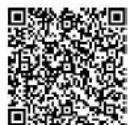
\includegraphics[width=0.85\linewidth]{images/2f48ee3d8430f6f264b7061923645647971dbad2de6f54f29b79eb72e10cba09.jpg}
\end{figure}


江西省卫生健康委员会职业健康处

签发日期025年071日

\subsubsection{江西省医学放射工作人员放射防护培训}

\subsubsection{合格证}

证书编号：142412010

证件号码：362201198409252615

所属专业：放射治疗(在岗)

从业单位：萍乡市人民医院

刘鲁根\_同志于\_2024年12月\_在放射防护在线培训平台完成规定学时任务，经考核合格，特发此证。

（该证书有效期贰年）

\begin{figure}[H]
\centering

\includegraphics[width=0.85\linewidth]{images/0cd8dc4c474c8c2a0e6964b9de56d3695a1c2ac6109be0e1bcf6f7c17f81f1ae.jpg}
\end{figure}


江西省卫生健康委员会职业健康处

签发日期2024年121日

\subsubsection{江西省医学放射工作人员放射防护培训}


证书编号：142412004

证件号码：36030219681102104X

所属专业：放射治疗（在岗）

从业单位：萍乡市人民医院

张红宇同志于2024年12月在放射防护在线培训平台完成规定学时任务，经考核合格，特发此证。

（该证书有效期贰年）

\begin{figure}[H]
\centering
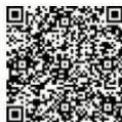
\includegraphics[width=0.85\linewidth]{images/3ce5be42ed0441b225c735b413309bdbce8fca7f0cf70d10bc46721e1ea37faf.jpg}
\end{figure}


江西省卫生健康委员会职业健康处

签发日期2024年12月19日

\subsubsection{江西省医学放射工作人员放射防护培训合格证}

证书编号：142507001

证件号码：360102197910213139

所属专业：放射治疗（在岗）

从业单位：萍乡市人民医院

欧阳公怒同志于2025年07月在放射防护在线培训平台完成规定学时任务，经考核合格，特发此证。

（该证书有效期贰年）

\begin{figure}[H]
\centering
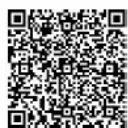
\includegraphics[width=0.85\linewidth]{images/a93f33494fdd7ec78bd0b4157ca24f4c8673cac454cef00e89477e7adce82f58.jpg}
\end{figure}


江西省卫生健康委员会职业健康处

签发日期025年0704日

\subsubsection{江西省医学放射工作人员放射防护培训}

\subsubsection{合格证}

证书编号：142506007

证件号码：360312198807153412

所属专业：放射治疗（在岗）

从业单位：萍乡市人民医院

辛焕中同志于2025年06月在放射防护在线培训平台完成规定学时任务，经考核合格，特发此证。

（该证书有效期贰年）

\begin{figure}[H]
\centering
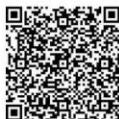
\includegraphics[width=0.85\linewidth]{images/5e5193f45dc56bee6ceb4a7a87f9e4ca07d8a2b8c607c0b17727208009654d72.jpg}
\end{figure}


江西省卫生健康委员会职业健康处

签发日期2025年06月29日

附件 9-3 本项目放射工作人员职业健康体检情况

体检类别：在岗期间

\subsubsection{放射工作人员职业健康检查表}

\begin{figure}[H]
\centering

\includegraphics[width=0.85\linewidth]{images/11ef69d428063470a1f015a7b002c02065a7d4f4232b7ce22b1329ff8c04fcd0.jpg}
\end{figure}


检查编号：681727

姓名：陈明伟

单位：萍乡市人民医院

身份证号：360302197411230517

联系电话：13979936063

检查日期：2025年07月22日

接害因素：电离辐射

\begin{figure}[H]
\centering
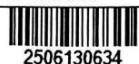
\includegraphics[width=0.85\linewidth]{images/5cc6fde4c839c6631c167cfc33bad44569e85b06e2024caab1ec752a831f68c3.jpg}
\end{figure}


姓名：陈明伟性别：男年龄：50登记流水：2506130634 体检日期：2025-06-16

\subsubsection{检查结果：}

*一般项目：

体重指数26.29：超重

*内科：

心率：80次/分

*外科：

腰围89cm

*胸部正位片：

双肺纹理粗多；请结合临床考虑。

*甲状腺彩超：

双叶甲状腺未见明显异常；

TI-RADS1类。

*上腹部彩超：

肝右叶小囊肿；

肝内脂肪浸润；

胆、脾、胰未见明显异常。

\subsubsection{体检结论：}

可继续原放射工作。

\subsubsection{处理意见：}

在检查周期内可以继续从事原放射岗位。

\subsubsection{主检医师：周莉萍}

\begin{figure}[H]
\centering
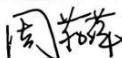
\includegraphics[width=0.85\linewidth]{images/2c3e89e3c19d62623a3fe44c62da63b0ab926283e2c97b72cd0dbb7669d920dd.jpg}
\end{figure}


\subsubsection{审核签发人：}

\begin{figure}[H]
\centering
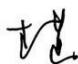
\includegraphics[width=0.85\linewidth]{images/674aa74c2afbaf2cb0d08ca6345dd65c8e0ab2995b24e39bdc22a42d6dffedeb.jpg}
\end{figure}


\subsubsection{体检}

\begin{figure}[H]
\centering
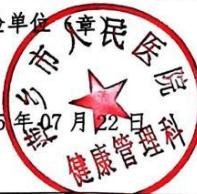
\includegraphics[width=0.85\linewidth]{images/3cdd570b4ad14e6926194b3afe369a5dcb5720e30572042006f5aad9484273d7.jpg}
\end{figure}


萍乡市人民医院

0799-6881753

第14页共14页

体检类别：在岗期间

\subsubsection{放射工作人员职业健康检查表}

\begin{figure}[H]
\centering

\includegraphics[width=0.85\linewidth]{images/5ad608e3c216166aedc67a4b32d5717183491c46cd7cd36b74efd50dc3b104a2.jpg}
\end{figure}


检查编号：646215

姓名：刘鲁根

单位：萍乡市人民医院

身份证号：362201198409252615

联系电话：18279929291

检查日期：2024年12月16日

接害因素：电离辐射

\begin{figure}[H]
\centering
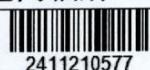
\includegraphics[width=0.85\linewidth]{images/e599e1e3f1cb2954e2ab3199228b9e656f39a5add1572d0272894da21342600e.jpg}
\end{figure}


姓名：刘鲁根性别：男年龄：40 登记流水：2411210577体检日期：2024-11-25

\subsubsection{检查结果：}

*一般项目：

体重指数24.54:超重

*血压：

血压143/84mmHg:血压偏高

*内科：

心率：68次/分

*外科：

腰围82cm

*胸部正位片：

右肺上野稍高密度影：增值性病灶可能，请结合临床。

*甲状腺彩超：

双叶甲状腺未见明显异常；

TI-RADS1类。

*腹部彩超：

肝内脂肪浸润；

胆、脾、胰未见明显异常。

\subsubsection{体检结论：}

可继续原放射工作。

\subsubsection{处理意见：}

在检查周期内可以继续从事原放射岗位。

主检医师：吴珊珊D

审核签发人：

体检单位2024年12月健康管理科

萍乡市人民医院

0799-6881753

第14页共14页

体检类别：在岗期间

\subsubsection{放射工作人员职业健康检查表}

\begin{figure}[H]
\centering

\includegraphics[width=0.85\linewidth]{images/a884c8ff1bbccd1ddd5afebd38b869d17bee2c951b54bcc94bae156ca01798a6.jpg}
\end{figure}


检查编号：681728

姓名：张红宇

单位：萍乡市人民医院

身份证号：36030219681102104X

联系电话：13879951567

检查日期：2025年07月22日

接害因素：电离辐射

\begin{figure}[H]
\centering
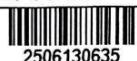
\includegraphics[width=0.85\linewidth]{images/e0b1118114c70a56168949d642340067de5f6a66a23668a14a62b240bcec54c1.jpg}
\end{figure}


姓名：张红宇性别：女年龄：56登记流水：2506130635体检日期：2025-06-17

\subsubsection{检查结果：}

*内科：

心率：75次/分

*外科：

腰围80cm

*尿液分析：

白细胞+-

*胸部正位片：

双肺纹理粗多；请结合临床考虑。

*甲状腺彩超：

双叶甲状腺未见明显异常；

TI-RADS1类。

*上腹部彩超：

肝、胆、脾、胰未见明显异常。

\subsubsection{体检结论：}

可继续原放射工作。

\subsubsection{处理意见：}

在检查周期内可以继续从事原放射岗位。

主检医师：周莉萍

\begin{figure}[H]
\centering
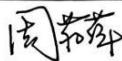
\includegraphics[width=0.85\linewidth]{images/0011eefbabdac46aaef4525093b810d9054727960baca0ddd83e76858b60beed.jpg}
\end{figure}


审核签发人：

\begin{figure}[H]
\centering
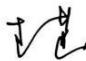
\includegraphics[width=0.85\linewidth]{images/c4e8d44358b19dd8213202b7d0ded705e2a4100650a0ea7558501d33ecb5d566.jpg}
\end{figure}


\begin{figure}[H]
\centering
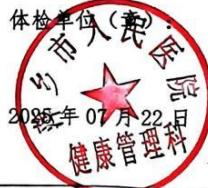
\includegraphics[width=0.85\linewidth]{images/e35e93b7773e9bf18c911a0fd1ce4c048e15aaa764207cdfc74b77ca1b997b2b.jpg}
\end{figure}


萍乡市人民医院

第14页共14页

0799-6881753

体检类别：在岗期间

\subsubsection{放射工作人员职业健康检查表}

\begin{figure}[H]
\centering

\includegraphics[width=0.85\linewidth]{images/bb2c461d5071d1ccf405b72082b419f6287c47cee536cc501ff4a0545b2498e4.jpg}
\end{figure}


检查编号：681729

姓名：辛焕中

单位：萍乡市人民医院

身份证号：360312198807153412

联系电话：13479855919

检查日期：2025年07月22日

接害因素：电离辐射

\begin{figure}[H]
\centering
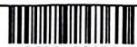
\includegraphics[width=0.85\linewidth]{images/8384f4b27fbbaba06914197a2f75c899a60737ee736073039154d203a625ed34.jpg}
\end{figure}


2506130636

姓名：亲焕中性别：男年龄：36登记流水：2506130636体检日期：2025-06-15

\subsubsection{检查结果：}

*一般项目：

体重指数25.64：超重

$^ *$内科：

心率：70次/分慢性病史：慢性肾炎3年，服药治疗。

*外科：

腰围80cm

*血常规：

红细胞（RBC)偏高 $( 6 . 2 9 * 1 0 \hat { \ } 1 2 / \mathrm { L } )$白细胞（WBC）偏高 $( 1 0 . 3 * 1 0 \ \hat { 9 } / \mathrm { L } )$淋巴细胞绝对值(LY\#）偏高（3.7*109/L）单核细胞绝对值（MO\#)偏高(1*109/L）平均红细胞血红蛋白含量（MCH）偏低(20.5 $1 * 1 0 \ \hat { \ } 9 / \mathrm { L } )$pg）血红蛋白浓度（HGB）偏低 $( 1 2 9 \ g / \mathrm { L } )$

*尿液分析：

尿隐血（BLD）3+尿蛋白质（PRO）2+

$^ *$胸部正位片：

肺内未见明显实质性病变。

$^ *$心电图：

1、窦性心律

2、I度房室传导阻滞

$^ *$甲状腺彩超：

双叶甲状腺未见明显异常；

TI-RADS1类。

*上腹部彩超：

脂肪肝；

肝内多发小囊肿；

胆、脾、胰未见明显异常。

\subsubsection{体检结论：}

可继续原放射工作。

\subsubsection{处理意见：}

在检查周期内可以继续从事原放射岗位。

主检医师：吴珊珊

审核签发人：

\begin{figure}[H]
\centering
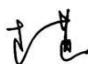
\includegraphics[width=0.85\linewidth]{images/2083862bf4a21cf899496aadf0e72fecf2d85663062c7769dd28847c2194c033.jpg}
\end{figure}


\begin{figure}[H]
\centering
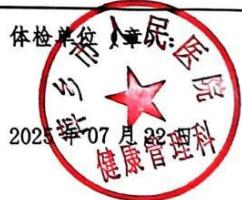
\includegraphics[width=0.85\linewidth]{images/ac6285e7797e12794a1079eafce03a779c30c5cfc29db429111bb311e41e7d42.jpg}
\end{figure}


萍乡市人民医院

0799-6881753

第14页共14页

体检类别：在岗期间

\subsubsection{放射工作人员职业健康检查表}

\begin{figure}[H]
\centering

\includegraphics[width=0.85\linewidth]{images/4accadbbe646bee2a3d1ca8b6a6c090bb2c944d08ec1af8894757b2f92e0d788.jpg}
\end{figure}


检查编号：619761

姓名：欧阳公怒

单位：萍乡市人民医院

身份证号：360102197910213139

联系电话：15907992510

检查日期：2024年08月06日

接害因素：电离辐射

\begin{figure}[H]
\centering
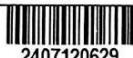
\includegraphics[width=0.85\linewidth]{images/ef888ab3d10b2de6477ab9bf43f94bfd2a4c3d3bdc98679855126e36952d1cff.jpg}
\end{figure}


姓名：欧阳公怒性别：男年龄：44登记流水：2407120629体检日期：2024-07-16

\subsubsection{检查结果：}

*一般项目：

体重指数27.72：超重

*内科：

心率：70次/分

*外科：

腰围82cm

*血常规：

单核细胞绝对值（MO\#）偏高 $( 0 . 7 * 1 0 \ \mathrm { \hat { ~ } 9 / L } )$

*胸部正位片：

双肺纹理粗多；请结合临床考虑。

*心电图：

1、窦性心动过缓

2、左室高电压

*甲状腺彩超：

双叶甲状腺未见明显异常；

TI-RADS1类。

*腹部彩超：

肝、胆、脾、胰未见明显异常。

\subsubsection{体检结论：}

可继续原放射工作。

\subsubsection{处理意见：}

在检查周期内可以继续从事原放射岗位。心血管内科就诊。

主检医师：周莉萍

\begin{figure}[H]
\centering
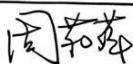
\includegraphics[width=0.85\linewidth]{images/7833ad367a44002afb7b83513369fb818794df8653c8e2ff47c939f305a8680d.jpg}
\end{figure}


审核签发人：

\begin{figure}[H]
\centering
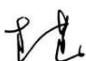
\includegraphics[width=0.85\linewidth]{images/09585fd8fa3a9d383cdab0eb292ab0158d4cf1aec4bd461bc12f3cf24f17f80c.jpg}
\end{figure}


体检单位

\begin{figure}[H]
\centering
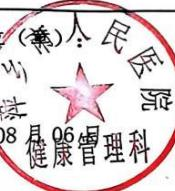
\includegraphics[width=0.85\linewidth]{images/73bf90f3cc04ecbc4e63610d81dce63cb96afe0e25c4f195546b6197a0617f31.jpg}
\end{figure}


2024年

第14页共14页

萍乡市人民医院

0799-6881753

附件9-4 个人剂量监测报告

\begin{figure}[H]
\centering

\includegraphics[width=0.85\linewidth]{images/e149ce66f1f9de4535d59f207a541a88395165ebb9f82edd1f054db51c70e522.jpg}
\end{figure}


\subsubsection{江西辐射剂量检测院有限公司}

\subsubsection{Radiation Dose Detection Research Institute of Jiangxi}

\subsubsection{检测报告}

\subsubsection{TEST REPORT}

\subsubsection{报告编号：赣检测院GR230498-04}

项目名称萍乡市人民医院职业外照射个人剂量检测

委托单位萍乡市人民医院

检测类型常规检测

报告日期2024年07月19日

\begin{figure}[H]
\centering
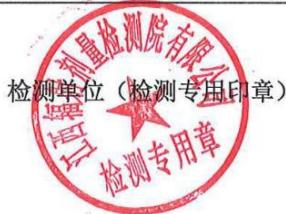
\includegraphics[width=0.85\linewidth]{images/bf372d731414ff2121e22eadede0d40a7da73d2c4fd9c6079d0600badfaba9db.jpg}
\end{figure}


地址：南昌市顺外路392号君嘉广场2号楼9楼西

邮编：330029

联系电话：19979186757、19979186693、0791-88225536

E-mail:jxfs2018@163.com

\subsubsection{明}

1.本公司坚持“独立、公正、科学、诚实”的服务理念，对检测数据负责。如有违反公正性、保密性的行为，给客户造成损失的，本公司愿意承担相应法律责任。
2.本报告无授权签字人签名无效（存档版无检测人、校核人、审核人、授权签字人签名无效）；涂改、增删、未盖公司检测专用章无效。
3.送样委托检测，本报告仅对来样负责。
4.本报告未经公司书面批准，不得部分复制本报告。本报告各页均为报告不可分割之部分，未经本公司同意，不得以任何方式作广告宣传。
5.若对本报告有异议者，请于收到报告之日起十五日内向我公司提出，逾期不予受理。

检测单位：江西辐射剂量检测院有限公司

联系地址：南昌市顺外路392号君嘉广场2号楼9楼西

邮政编码：330029

联系电话：19979186757、19979186693、0791-88225536

E-mail:jxfs2018@163.com

报告编号：赣检测院GR2230498-04

\begin{figure}[H]
\centering

\includegraphics[width=0.85\linewidth]{images/c5127604b9cbbe39e85faf77489dfb0311b3f73b0ec2e81368767361f9a286f5.jpg}
\end{figure}


\subsubsection{江西辐射剂量检测院有限公司}

\subsubsection{Radiation Dose Detection Research Institute of Jiangxi}

检测报告
样品受理编号：230498-04

\begin{table}[H]
\centering
\begin{tabular}{|c|c|c|c|}
\hline
检测项目 & 职业外照射个人剂量检测 & 检测方法 & 热释光监测方法 \\
\hline
用人单位 & 萍乡市人民医院 & 委托单位 & 萍乡市人民医院 \\
\hline
收样日期 & 2024-07-12 & 检测日期 & 2024-07-15 \\
\hline
检测/评价依据 & GBZ 128-2019职业性外照射个人监测规范 &  &  \\
\hline
GB 18871-2002电离辐射防护与辐射源安全基本标准 &  &  &  \\
\hline
检测室名称 & 个人剂量室 & 检测类别/目的 & 委托检测/常规检测 \\
\hline
检测仪器名称/型号/编号 & 热释光剂量读出器 / BRGD2000-D / JXFS/YQ-029 &  &  \\
\hline
检测仪器检定/校准信息 & 上海市计量测试技术研究院华东国家计量测试中心证书编号:2024H21-10-5338218001证书有效期至:2025年3月21日 &  &  \\
\hline
探测器 & 热释光剂量计(TLD)-片状(圆片)-LiF(MgCuP) & 样品总数 & 139人份 \\
\hline
剂量限值 & 放射工作人员在正常情况下的职业照射水平应不超过GB 18871-2002《电离辐射防护与辐射源安全基本标准》所规定的以下限值:1、连续5年的年平均有效剂量,20mSv;2、任何1年中的有效剂量,50mSv。 &  &  \\
\hline
检测结果 & 详见表1。 & 监测的量 & Hp(10) \\
\hline
(编制人:徐梦颖)授权签字人 空 &  &  &  \\
\hline
签发日期 2024年7月19日 &  &  &  \\
\hline
检测单位(检测专用印章) &  &  &  \\
\hline
\end{tabular}
\end{table}


报告编号：赣检测院GR2230498-04

表 $^ 1$放射工作人员职业性外照射个人剂量检测结果

\begin{table}[H]
\centering
\begin{tabular}{|c|c|c|c|c|c|c|c|}
\hline
样品编号 & 姓名 & 性别 & 职业类别 & 剂量计佩戴起始日期 & 剂量计佩戴终止日期 & 佩戴周期(月) & 个人剂量当量Hp(10)(mSv) \\
\hline
360301005001 & 邹南安 & 男 & 诊断放射学(2A) & 24-4-1 & 24-6-30 & 三个月 & 0.12 \\
\hline
360301005002 & 巫启恒 & 男 & 诊断放射学(2A) & 24-4-1 & 24-6-30 & 三个月 & 0.01* \\
\hline
360301005003 & 黎瑛 & 女 & 诊断放射学(2A) & 24-4-1 & 24-6-30 & 三个月 & 0.07 \\
\hline
360301005004 & 刘峰 & 男 & 诊断放射学(2A) & 24-4-1 & 24-6-30 & 三个月 & 0.10 \\
\hline
360301005005 & 刘小红 & 女 & 诊断放射学(2A) & 24-4-1 & 24-6-30 & 三个月 & 0.03 \\
\hline
360301005006 & 李丰章 & 男 & 诊断放射学(2A) & 24-4-1 & 24-6-30 & 三个月 & 0.01* \\
\hline
360301005007 & 黄元发 & 男 & 诊断放射学(2A) & 24-4-1 & 24-6-30 & 三个月 & 0.01* \\
\hline
360301005010 & 曾志宏 & 男 & 诊断放射学(2A) & 24-4-1 & 24-6-30 & 三个月 & 0.01* \\
\hline
360301005011 & 谭华 & 男 & 诊断放射学(2A) & 24-4-1 & 24-6-30 & 三个月 & 0.01* \\
\hline
360301005012 & 陈萍赣 & 男 & 诊断放射学(2A) & 24-4-1 & 24-6-30 & 三个月 & 0.01* \\
\hline
360301005013 & 郭欣 & 男 & 诊断放射学(2A) & 24-4-1 & 24-6-30 & 三个月 & 0.10 \\
\hline
360301005014 & 钟自华 & 男 & 诊断放射学(2A) & 24-4-1 & 24-6-30 & 三个月 & 0.12 \\
\hline
360301005015 & 陈洋勇 & 男 & 诊断放射学(2A) & 24-4-1 & 24-6-30 & 三个月 & 0.03\# \\
\hline
360301005016 & 刘霞 & 女 & 诊断放射学(2A) & 24-4-1 & 24-6-30 & 三个月 & 0.01* \\
\hline
360301005017 & 陈亮 & 男 & 诊断放射学(2A) & 24-4-1 & 24-6-30 & 三个月 & 0.01* \\
\hline
360301005018 & 傅志颖 & 女 & 诊断放射学(2A) & 24-4-1 & 24-6-30 & 三个月 & 0.01* \\
\hline
360301005020 & 李琪 & 男 & 诊断放射学(2A) & 24-4-1 & 24-6-30 & 三个月 & 0.01* \\
\hline
360301005021 & 周晶 & 女 & 诊断放射学(2A) & 24-4-1 & 24-6-30 & 三个月 & 0.01* \\
\hline
360301005022 & 肖维国 & 男 & 诊断放射学(2A) & 24-4-1 & 24-6-30 & 三个月 & 0.10 \\
\hline
360301005023 & 刘天笑 & 女 & 诊断放射学(2A) & 24-4-1 & 24-6-30 & 三个月 & 0.01* \\
\hline
360301005024 & 胡含明 & 男 & 诊断放射学(2A) & 24-4-1 & 24-6-30 & 三个月 & 0.03\# \\
\hline
360301005026 & 王敬鹏 & 男 & 诊断放射学(2A) & 24-4-1 & 24-6-30 & 三个月 & 0.15 \\
\hline
360301005027 & 王爱华 & 女 & 诊断放射学(2A) & 24-4-1 & 24-6-30 & 三个月 & 0.14 \\
\hline
360301005028 & 崔甜甜 & 女 & 诊断放射学(2A) & 24-4-1 & 24-6-30 & 三个月 & 0.01* \\
\hline
360301005029 & 杜红 & 女 & 诊断放射学(2A) & 24-4-1 & 24-6-30 & 三个月 & 0.01* \\
\hline
360301005030 & 文翠 & 女 & 诊断放射学(2A) & 24-4-1 & 24-6-30 & 三个月 & 0.01* \\
\hline
360301005031 & 易鑫 & 男 & 诊断放射学(2A) & 24-4-1 & 24-6-30 & 三个月 & 0.01* \\
\hline
360301005032 & 贺曦 & 男 & 诊断放射学(2A) & 24-4-1 & 24-6-30 & 三个月 & 0.01* \\
\hline
\end{tabular}
\end{table}


报告编号：赣检测院GR2230498-04


\begin{table}[H]
\centering
\begin{tabular}{|c|c|c|c|c|c|c|c|c|}
\hline
360301005033 & 万红 & 女 & 诊断放射学(2A) & 24-4-1 & 24-6-30 & 三个月 & 0.03 &  \\
\hline
360301005034 & 廖林 & 女 & 诊断放射学(2A) & 24-4-1 & 24-6-30 & 三个月 & 0.04 &  \\
\hline
360301005035 & 张晓玲 & 女 & 诊断放射学(2A) & 24-4-1 & 24-6-30 & 三个月 & 0.01* &  \\
\hline
360301005036 & 黎安琪 & 女 & 诊断放射学(2A) & 24-4-1 & 24-6-30 & 三个月 & 0.01* &  \\
\hline
360301005037 & 吴正波 & 男 & 诊断放射学(2A) & 24-4-1 & 24-6-30 & 三个月 & 0.01* &  \\
\hline
360301005038 & 王德华 & 男 & 诊断放射学(2A) & 24-4-1 & 24-6-30 & 三个月 & 0.01* &  \\
\hline
360301005039 & 吴斌 & 男 & 诊断放射学(2A) & 24-4-1 & 24-6-30 & 三个月 & 0.05 &  \\
\hline
360301005040 & 易阳 & 女 & 诊断放射学(2A) & 24-4-1 & 24-6-30 & 三个月 & 0.10 &  \\
\hline
360301005041 & 汤裕兵 & 男 & 诊断放射学(2A) & 24-4-1 & 24-6-30 & 三个月 & 0.01* &  \\
\hline
360301005042 & 黄瑶 & 女 & 诊断放射学(2A) & 24-4-1 & 24-6-30 & 三个月 & 0.01* &  \\
\hline
360301005044 & 雍妤琴 & 女 & 诊断放射学(2A) & 24-4-1 & 24-6-30 & 三个月 & 0.09 &  \\
\hline
360301005046 & 杨迪 & 女 & 诊断放射学(2A) & 24-4-1 & 24-6-30 & 三个月 & 0.01* &  \\
\hline
360301005048 & 李鹏 & 男 & 核医学(2C) & 24-4-1 & 24-6-30 & 三个月 & 0.08 &  \\
\hline
360301005049 & 杨凭飞 & 男 & 核医学(2C) & 24-4-1 & 24-6-30 & 三个月 & 0.03 &  \\
\hline
360301005050 & 文晓琴 & 女 & 核医学(2C) & 24-4-1 & 24-6-30 & 三个月 & 0.09 &  \\
\hline
360301005051 & 黎心四 & 男 & 核医学(2C) & 24-4-1 & 24-6-30 & 三个月 & 0.12 &  \\
\hline
360301005052 & 张西 & 女 & 核医学(2C) & 24-4-1 & 24-6-30 & 三个月 & 0.10 &  \\
\hline
360301005053 & 王健 & 男 & 核医学(2C) & 24-4-1 & 24-6-30 & 三个月 & 0.06 &  \\
\hline
360301005054 & 陈明伟 & 男 & 放射治疗(2D) & 24-4-1 & 24-6-30 & 三个月 & 0.01* &  \\
\hline
360301005055 & 黄华堂 & 男 & 放射治疗(2D) & 24-4-1 & 24-6-30 & 三个月 & 0.01* &  \\
\hline
360301005056 & 张红宇 & 女 & 放射治疗(2D) & 24-4-1 & 24-6-30 & 三个月 & 0.03 &  \\
\hline
360301005057 & 辛焕中 & 男 & 放射治疗(2D) & 24-4-1 & 24-6-30 & 三个月 & 0.02 &  \\
\hline
360301005058 & 胡依冰 & 女 & 放射治疗(2D) & 24-4-1 & 24-6-30 & 三个月 & 0.01* &  \\
\hline
360301005059 & 刘鲁根 & 男 & 放射治疗(2D) & 24-4-1 & 24-6-30 & 三个月 & 0.01* &  \\
\hline
360301005060 & 乔浩 & 男 & 放射治疗(2D) & 24-4-1 & 24-6-30 & 三个月 & 0.02 &  \\
\hline
360301005061 & 董文哲 & 男 & 介入放射学(2E) & 24-4-1 & 24-6-30 & 三个月 & 铅衣内 & 0.01* \\
\hline
铅衣外 & 0.01* &  &  &  &  &  &  &  \\
\hline
360301005063 & 肖江 & 女 & 介入放射学(2E) & 24-4-1 & 24-6-30 & 三个月 & 铅衣内 & 0.01* \\
\hline
铅衣外 & 0.01* &  &  &  &  &  &  &  \\
\hline
360301005064 & 廖延亮 & 男 & 诊断放射学(2A) & 24-4-1 & 24-6-30 & 三个月 & 0.01* &  \\
\hline
360301005065 & 郑磊 & 男 & 介入放射学(2E) & 24-4-1 & 24-6-30 & 三个月 & 铅衣内 & 0.01* \\
\hline
铅衣外 & 0.01* &  &  &  &  &  &  &  \\
\hline
360301005066 & 林婷 & 女 & 介入放射学(2E) & 24-4-1 & 24-6-30 & 三个月 & 铅衣内 & 0.01* \\
\hline
铅衣外 & 0.01* &  &  &  &  &  &  &  \\
\hline
\end{tabular}
\end{table}


报告编号：赣检测院GR2230498-04


\begin{table}[H]
\centering
\begin{tabular}{|c|c|c|c|c|c|c|c|c|}
\hline
360301005067 & 周春春 & 女 & 介入放射学(2E) & 24-4-1 & 24-6-30 & 三个月 & 铅衣内 & 0.01* \\
\hline
铅衣外 & 0.04 &  &  &  &  &  &  &  \\
\hline
360301005068 & 杨侃 & 男 & 介入放射学(2E) & 24-4-1 & 24-6-30 & 三个月 & 铅衣内 & 0.01* \\
\hline
铅衣外 & 0.01* &  &  &  &  &  &  &  \\
\hline
360301005069 & 易瀚杰 & 男 & 介入放射学(2E) & 24-4-1 & 24-6-30 & 三个月 & 铅衣内 & 0.01* \\
\hline
铅衣外 & 0.01* &  &  &  &  &  &  &  \\
\hline
360301005070 & 刘晨曦 & 女 & 介入放射学(2E) & 24-4-1 & 24-6-30 & 三个月 & 铅衣内 & 0.01*\# \\
\hline
铅衣外 & 0.01*\# &  &  &  &  &  &  &  \\
\hline
360301005071 & 韩涛 & 男 & 介入放射学(2E) & 24-4-1 & 24-6-30 & 三个月 & 铅衣内 & 0.06 \\
\hline
铅衣外 & 2.98 &  &  &  &  &  &  &  \\
\hline
360301005072 & 廖骞 & 男 & 介入放射学(2E) & 24-4-1 & 24-6-30 & 三个月 & 铅衣内 & 0.01* \\
\hline
铅衣外 & 0.01* &  &  &  &  &  &  &  \\
\hline
360301005073 & 蔡恒烈 & 男 & 介入放射学(2E) & 24-4-1 & 24-6-30 & 三个月 & 铅衣内 & 0.29 \\
\hline
铅衣外 & 9.91 &  &  &  &  &  &  &  \\
\hline
360301005074 & 王奕 & 男 & 介入放射学(2E) & 24-4-1 & 24-6-30 & 三个月 & 铅衣内 & 0.01* \\
\hline
铅衣外 & 0.01* &  &  &  &  &  &  &  \\
\hline
360301005075 & 张志强 & 男 & 介入放射学(2E) & 24-4-1 & 24-6-30 & 三个月 & 铅衣内 & 0.01* \\
\hline
铅衣外 & 5.90 &  &  &  &  &  &  &  \\
\hline
360301005076 & 崔钢 & 男 & 介入放射学(2E) & 24-4-1 & 24-6-30 & 三个月 & 铅衣内 & 0.07\# \\
\hline
铅衣外 & 3.76\# &  &  &  &  &  &  &  \\
\hline
360301005077 & 龚敏 & 男 & 介入放射学(2E) & 24-4-1 & 24-6-30 & 三个月 & 铅衣内 & 0.01* \\
\hline
铅衣外 & 0.01* &  &  &  &  &  &  &  \\
\hline
360301005078 & 韩明 & 男 & 介入放射学(2E) & 24-4-1 & 24-6-30 & 三个月 & 铅衣内 & 0.01* \\
\hline
铅衣外 & 0.01* &  &  &  &  &  &  &  \\
\hline
360301005080 & 许优 & 女 & 核医学(2C) & 24-4-1 & 24-6-30 & 三个月 & 0.08 &  \\
\hline
360301005081 & 贺娇 & 女 & 介入放射学(2E) & 24-4-1 & 24-6-30 & 三个月 & 铅衣内 & 0.01* \\
\hline
铅衣外 & 0.01* &  &  &  &  &  &  &  \\
\hline
360301005082 & 朱勇美 & 女 & 介入放射学(2E) & 24-4-1 & 24-6-30 & 三个月 & 铅衣内 & 0.01* \\
\hline
铅衣外 & 0.01* &  &  &  &  &  &  &  \\
\hline
360301005084 & 付云辉 & 男 & 介入放射学(2E) & 24-4-1 & 24-6-30 & 三个月 & 铅衣内 & 0.01* \\
\hline
铅衣外 & 0.01* &  &  &  &  &  &  &  \\
\hline
360301005085 & 黄文军 & 男 & 介入放射学(2E) & 24-4-1 & 24-6-30 & 三个月 & 铅衣内 & 0.01* \\
\hline
铅衣外 & 0.01* &  &  &  &  &  &  &  \\
\hline
360301005087 & 周国忠 & 男 & 介入放射学(2E) & 24-4-1 & 24-6-30 & 三个月 & 铅衣内 & 0.01* \\
\hline
铅衣外 & 0.01* &  &  &  &  &  &  &  \\
\hline
360301005089 & 罗勤 & 男 & 介入放射学(2E) & 24-4-1 & 24-6-30 & 三个月 & 铅衣内 & 0.3\# \\
\hline
铅衣外 & 3.22 &  &  &  &  &  &  &  \\
\hline
360301005090 & 张雨虹 & 男 & 介入放射学(2E) & 24-4-1 & 24-6-30 & 三个月 & 铅衣内 & 0.03 \\
\hline
铅衣外 & 0.56 &  &  &  &  &  &  &  \\
\hline
360301005091 & 曾广忠 & 男 & 介入放射学(2E) & 24-4-1 & 24-6-30 & 三个月 & 铅衣内 & 0.01* \\
\hline
铅衣外 & 0.01* &  &  &  &  &  &  &  \\
\hline
360301005092 & 姚常 & 男 & 介入放射学(2E) & 24-4-1 & 24-6-30 & 三个月 & 铅衣内 & 1.47 \\
\hline
铅衣外 & 0.65\# &  &  &  &  &  &  &  \\
\hline
\end{tabular}
\end{table}


报告编号：赣检测院GR2230498-04

\begin{table}[H]
\centering
\begin{tabular}{|c|c|c|c|c|c|c|c|c|}
\hline
360301005093 & 彭阳 & 男 & 介入放射学(2E) & 24-4-1 & 24-6-30 & 三个月 & 铅衣内 & 0.01* \\
\hline
铅衣外 & 0.01* &  &  &  &  &  &  &  \\
\hline
360301005095 & 赖丹 & 男 & 介入放射学(2E) & 24-4-1 & 24-6-30 & 三个月 & 铅衣内 & 0.01* \\
\hline
铅衣外 & 0.01* &  &  &  &  &  &  &  \\
\hline
360301005096 & 毛云飞 & 男 & 介入放射学(2E) & 24-4-1 & 24-6-30 & 三个月 & 铅衣内 & 0.01* \\
\hline
铅衣外 & 1.13 &  &  &  &  &  &  &  \\
\hline
360301005097 & 李洛 & 男 & 介入放射学(2E & 24-4-1 & 24-6-30 & 三个月 & 铅衣内 & 0.02 \\
\hline
铅衣外 & 1.50 &  &  &  &  &  &  &  \\
\hline
360301005100 & 朱飞 & 男 & 介入放射学(2E) & 24-4-1 & 24-6-30 & 三个月 & 铅衣内 & 0.73\# \\
\hline
铅衣外 & 1.30\# &  &  &  &  &  &  &  \\
\hline
360301005101 & 丁绍纯 & 男 & 介入放射学(2E) & 24-4-1 & 24-6-30 & 三个月 & 铅衣内 & 0.73 \\
\hline
铅衣外 & 1.30 &  &  &  &  &  &  &  \\
\hline
360301005102 & 王稻 & 男 & 介入放射学(2E) & 24-4-1 & 24-6-30 & 三个月 & 铅衣内 & 0.56 \\
\hline
铅衣外 & 0.69 &  &  &  &  &  &  &  \\
\hline
360301005103 & 刘灏灏 & 男 & 介入放射学(2E) & 24-4-1 & 24-6-30 & 三个月 & 铅衣内 & 0.01* \\
\hline
铅衣外 & 0.01* &  &  &  &  &  &  &  \\
\hline
360301005104 & 王俊东 & 男 & 介入放射学(2E) & 24-4-1 & 24-6-30 & 三个月 & 铅衣内 & 0.01* \\
\hline
铅衣外 & 0.01* &  &  &  &  &  &  &  \\
\hline
360301005105 & 廖鹏 & 男 & 介入放射学(2E) & 24-4-1 & 24-6-30 & 三个月 & 铅衣内 & 0.01* \\
\hline
铅衣外 & 0.01* &  &  &  &  &  &  &  \\
\hline
360301005106 & 蔡坤豪 & 男 & 诊断放射学(2A) & 24-4-1 & 24-6-30 & 三个月 & 0.01* &  \\
\hline
360301005108 & 欧阳公怒 & 男 & 其它(2F) & 24-4-1 & 24-6-30 & 三个月 & 0.01* &  \\
\hline
360301005109 & 贺小张 & 男 & 介入放射学(2E) & 24-4-1 & 24-6-30 & 三个月 & 铅衣内 & 0.01* \\
\hline
铅衣外 & 0.01* &  &  &  &  &  &  &  \\
\hline
360301005110 & 许绍林 & 男 & 介入放射学(2E) & 24-4-1 & 24-6-30 & 三个月 & 铅衣内 & 0.01* \\
\hline
铅衣外 & 0.01* &  &  &  &  &  &  &  \\
\hline
360301005112 & 龙阳天利 & 女 & 诊断放射学(2A) & 24-4-1 & 24-6-30 & 三个月 & 0.01* &  \\
\hline
360301005113 & 李健 & 男 & 诊断放射学(2A) & 24-4-1 & 24-6-30 & 三个月 & 0.01* &  \\
\hline
360301005114 & 叶作增 & 男 & 诊断放射学(2A) & 24-4-1 & 24-6-30 & 三个月 & 0.01* &  \\
\hline
360301005115 & 周礼平 & 男 & 诊断放射学(2A) & 24-4-1 & 24-6-30 & 三个月 & 0.01* &  \\
\hline
360301005116 & 黄丽 & 女 & 诊断放射学(2A) & 24-4-1 & 24-6-30 & 三个月 & 0.03\# &  \\
\hline
360301005117 & 糜洪 & 男 & 诊断放射学(2A) & 24-4-1 & 24-6-30 & 三个月 & 0.01* &  \\
\hline
360301005121 & 朱敏 & 女 & 介入放射学(2E) & 24-4-1 & 24-6-30 & 三个月 & 铅衣内 & 0.01* \\
\hline
铅衣外 & 0.01* &  &  &  &  &  &  &  \\
\hline
360301005122 & 李晨 & 男 & 介入放射学(2E) & 24-4-1 & 24-6-30 & 三个月 & 铅衣内 & 0.02\# \\
\hline
铅衣外 & 4.23 &  &  &  &  &  &  &  \\
\hline
360301005124 & 廖晓慧 & 女 & 诊断放射学(2A) & 24-4-1 & 24-6-30 & 三个月 & 0.01* &  \\
\hline
360301005125 & 邓莎 & 女 & 诊断放射学(2A) & 24-4-1 & 24-6-30 & 三个月 & 0.01* &  \\
\hline
360301005126 & 易江 & 男 & 诊断放射学(2A) & 24-4-1 & 24-6-30 & 三个月 & 0.01* &  \\
\hline
\end{tabular}
\end{table}


报告编号：赣检测院GR2230498-04


\begin{table}[H]
\centering
\begin{tabular}{|c|c|c|c|c|c|c|c|c|}
\hline
360301005127 & 刘建刚 & 男 & 介入放射学(2E) & 24-4-1 & 24-6-30 & 三个月 & 铅衣内 & 0.01* \\
\hline
铅衣外 & 0.01* &  &  &  &  &  &  &  \\
\hline
360301005128 & 刘霞 & 女 & 介入放射学(2E) & 24-4-1 & 24-6-30 & 三个月 & 铅衣内 & 0.01*\# \\
\hline
铅衣外 & 0.01*\# &  &  &  &  &  &  &  \\
\hline
360301005129 & 彭治鹏 & 男 & 介入放射学(2E) & 24-4-1 & 24-6-30 & 三个月 & 铅衣内 & 0.01* \\
\hline
铅衣外 & 0.01* &  &  &  &  &  &  &  \\
\hline
360301005130 & 兰前鑫 & 男 & 介入放射学(2E) & 24-4-1 & 24-6-30 & 三个月 & 铅衣内 & 0.01*\# \\
\hline
铅衣外 & 0.01* &  &  &  &  &  &  &  \\
\hline
360301005131 & 刘兴龙 & 男 & 介入放射学(2E) & 24-4-1 & 24-6-30 & 三个月 & 铅衣内 & 0.01* \\
\hline
铅衣外 & 0.01* &  &  &  &  &  &  &  \\
\hline
360301005133 & 彭成福 & 男 & 介入放射学(2E) & 24-4-1 & 24-6-30 & 三个月 & 铅衣内 & 0.24 \\
\hline
铅衣外 & 0.88\# &  &  &  &  &  &  &  \\
\hline
360301005134 & 孙芬芬 & 女 & 介入放射学(2E) & 24-4-1 & 24-6-30 & 三个月 & 铅衣内 & 0.01* \\
\hline
铅衣外 & 0.01* &  &  &  &  &  &  &  \\
\hline
360301005135 & 彭向丽 & 女 & 诊断放射学(2A) & 24-4-1 & 24-6-30 & 三个月 & 0.01* &  \\
\hline
360301005136 & 任妹 & 女 & 核医学(2C) & 24-4-1 & 24-6-30 & 三个月 & 0.04 &  \\
\hline
360301005137 & 唐志武 & 男 & 诊断放射学(2A) & 24-4-1 & 24-6-30 & 三个月 & 0.05 &  \\
\hline
360301005138 & 揭继斯 & 男 & 诊断放射学(2A) & 24-4-1 & 24-6-30 & 三个月 & 0.01* &  \\
\hline
360301005139 & 龙安友 & 男 & 诊断放射学(2A) & 24-4-1 & 24-6-30 & 三个月 & 0.01* &  \\
\hline
360301005140 & 周宇煊 & 男 & 诊断放射学(2A) & 24-4-1 & 24-6-30 & 三个月 & 0.01* &  \\
\hline
360301005141 & 陈智勇 & 男 & 诊断放射学(2A) & 24-4-1 & 24-6-30 & 三个月 & 0.07 &  \\
\hline
360301005142 & 何婷 & 女 & 诊断放射学(2A) & 24-4-1 & 24-6-30 & 三个月 & 0.03 &  \\
\hline
360301005143 & 张崇海 & 男 & 诊断放射学(2A) & 24-4-1 & 24-6-30 & 三个月 & 0.04 &  \\
\hline
360301005144 & 黄紫娴 & 女 & 诊断放射学(2A) & 24-4-1 & 24-6-30 & 三个月 & 0.01* &  \\
\hline
360301005145 & 黄珍 & 女 & 介入放射学(2E) & 24-4-1 & 24-6-30 & 三个月 & 0.01* &  \\
\hline
360301005146 & 李苏琴 & 女 & 介入放射学(2E) & 24-4-1 & 24-6-30 & 三个月 & 铅衣内 & 0.01*\# \\
\hline
铅衣外 & 0.01*\# &  &  &  &  &  &  &  \\
\hline
360301005148 & 吴朝 & 男 & 介入放射学(2E) & 24-4-1 & 24-6-30 & 三个月 & 铅衣内 & 0.01* \\
\hline
铅衣外 & 0.01* &  &  &  &  &  &  &  \\
\hline
360301005149 & 郑旺 & 男 & 介入放射学(2E) & 24-4-1 & 24-6-30 & 三个月 & 铅衣内 & 0.01* \\
\hline
铅衣外 & 0.01* &  &  &  &  &  &  &  \\
\hline
360301005150 & 陈娇 & 女 & 核医学(2C) & 24-4-1 & 24-6-30 & 三个月 & 0.09 &  \\
\hline
360301005151 & 邱明涛 & 男 & 介入放射学(2E) & 24-4-1 & 24-6-30 & 三个月 & 铅衣内 & 0.01* \\
\hline
铅衣外 & 4.59 &  &  &  &  &  &  &  \\
\hline
360301005158 & 严兵 & 男 & 介入放射学(2E) & 24-4-1 & 24-6-30 & 三个月 & 铅衣内 & 0.01* \\
\hline
铅衣外 & 3.76\# &  &  &  &  &  &  &  \\
\hline
360301005162 & 周慧 & 女 & 核医学(2C) & 24-4-1 & 24-6-30 & 三个月 & 0.09 &  \\
\hline
360301005163 & 王敏 & 女 & 诊断放射学(2A) & 24-4-1 & 24-6-30 & 三个月 & 0.01* &  \\
\hline
\end{tabular}
\end{table}


报告编号：赣检测院GR2230498-04


\begin{table}[H]
\centering
\begin{tabular}{|c|c|c|c|c|c|c|c|c|}
\hline
360301005164 & 杨道益 & 男 & 诊断放射学(2A) & 24-4-1 & 24-6-30 & 三个月 & 0.01* &  \\
\hline
360301005165 & 沈雯婷 & 女 & 诊断放射学(2A) & 24-4-1 & 24-6-30 & 三个月 & 0.01* &  \\
\hline
360301005166 & 彭其 & 女 & 诊断放射学(2A) & 24-4-1 & 24-6-30 & 三个月 & 0.01* &  \\
\hline
360301005167 & 刘涛 & 男 & 诊断放射学(2A) & 24-4-1 & 24-6-30 & 三个月 & 0.01* &  \\
\hline
360301005168 & 闫博宇 & 男 & 介入放射学(2E) & 24-4-1 & 24-6-30 & 三个月 & 铅衣内 & 0.09 \\
\hline
铅衣外 & 0.63 &  &  &  &  &  &  &  \\
\hline
360301005169 & 陈小根 & 男 & 介入放射学(2E) & 24-4-1 & 24-6-30 & 三个月 & 铅衣内 & 0.01* \\
\hline
铅衣外 & 0.01* &  &  &  &  &  &  &  \\
\hline
360301005170 & 邱萍 & 女 & 诊断放射学(2A) & 24-4-1 & 24-6-30 & 三个月 & 0.01* &  \\
\hline
360301005171 & 张涵茹 & 女 & 介入放射学(2E) & 24-4-1 & 24-6-30 & 三个月 & 铅衣内 & 0.01* \\
\hline
铅衣外 & 0.01* &  &  &  &  &  &  &  \\
\hline
360301005 & 对照剂量计 & / & / & 24-4-1 & 24-6-30 & 三个月 & 0.31 &  \\
\hline
(以下空白) &  &  &  &  &  &  &  &  \\
\hline
\end{tabular}
\end{table}


备注：1.“职业类别”详见GBZ128-2019附录C中表C.1；
2.H（10）适用于体表下10mm深处的器官或组织的监测；
3.本周期的调查水平参考值为：1.25mSv；
3底的L）为01，标注的检测结果小于DL，为便于职业照射统计 $0 , 0 2 \mathrm { m S v }$应的剂量档案中记录为1/2MDL；
5.当用人单位工作人员佩戴的剂量计确认已经丢失、损坏、因故得不到读数或所得读数不正确反映工作人员所接受的剂量时，则出具名义剂量，并在数据后标注“\#”；如果工作人员本期的剂量值超过本周期调查水平，则在数据后标注“△”。
6.\#标注的结果为名义剂量：360301005076崔钢（内）360301005076崔钢（外）360301005100朱飞（内）360301005100朱飞（外）本周期个人剂量当量检测结果超周期调查水平，经调查非其真实值：360301005015陈洋勇360301005024胡含明360301005116黄丽360301005070刘晨曦（内）360301005070刘晨曦（外）360301005128刘霞（内）360301005128刘霞（外）360301005146李苏琴（内）360301005146李苏琴（外）360301005089罗勤（内）360301005092姚常（外）360301005122李晨（内）360301005130兰前鑫（内）360301005133彭成福（外）360301005158严兵（外）本周期剂量计遗失。
7.以上检测结果仅对本次检测有效，已扣除本底。

\begin{figure}[H]
\centering

\includegraphics[width=0.85\linewidth]{images/e5b104ec0486d50c5d37248b32c006e3cb1af0e815f48d843a6a3f84505a97b1.jpg}
\end{figure}


\subsubsection{湖南合润检测技术有限公司}

\subsubsection{HUNAN HERUN TESTING TECHNOLOGY CO.,LTD}

\begin{figure}[H]
\centering

\includegraphics[width=0.85\linewidth]{images/7c5f977dbd22221cb03d0663eb68df7a56d409effec2a5ce67e01ab999fa4e4d.jpg}
\end{figure}


211803102214

\subsubsection{检测报告}

\subsubsection{TEST REPORT}

报告编号：

Report No.

24HRJLW0038Q04

检测项目：

Test items

X/y射线外照射个人剂量监测 $H \mathfrak { p } ( 1 0 )$

检测类型：

Detection type

委托监测/常规监测

委托单位：

Client

萍乡市人民医院

样品名称：

Samplename

\begin{figure}[H]
\centering
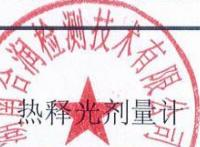
\includegraphics[width=0.85\linewidth]{images/d90baff58e512652ba18a2975b2d2c3214e38c0379623efeaee55d45d8fde996.jpg}
\end{figure}


报告日期：

Date ofReport

检验检测专用章

2025年2月10日

\begin{figure}[H]
\centering

\includegraphics[width=0.85\linewidth]{images/4114c2090cfa84ac58a1934f82ad4aaacd31a6d151f5de173595e8f04d427273.jpg}
\end{figure}


\subsubsection{注意事项}

\subsubsection{CONSIDERATIONS}

1.本报告无检验检测机构“检测报告专用章”无效。
2.本报告无“CMA”标志不具备法律证明作用。
3.复制本报告未重新加盖“检测报告专用章”无效。
4.本报告无报告签发人（授权签字人）签名无效。
5.本报告涂改无效。
6.对本检验报告若有异议，应于收到报告之日起十五日内向检验单位提出，逾期不予受理。
7.本报告仅对所委托检测的样品负责。
8.本报告解释权归检验检测单位。

声明：湖南合润检测技术有限公司为独立的第三方检测机构，公司规定全体员工必须遵守以下声明要求：

准确满意的服务；
\begin{enumerate}
\item 本公司及公司全体人员不得与其从事的检验检测活动以及出具的数据和结果存在利益关系：绝不参
\end{enumerate}

\subsubsection{检测报告}

\subsubsection{REPORTOFTEST}

报告编号：

Report No.

24HRJLW0038Q04

委托单位：

Client

1.本次监测的主要技术依据(Reference documents for the test)：

《职业性外照射个人监测监测规范》（GBZ128—2019）

《电离辐射防护与放射源安全基本标准》（GB18871—2002）

2.本次监测的环境条件(Environmentcondition forthe test)：

53\%RH

3.本次监测所使用的主要测量设备(Main standards ofmeasurement used in the test)：

\begin{table}[H]
\centering
\begin{tabular}{|c|c|c|c|}
\hline
名称/型号 & 编号 & 证书号/有效期 & 溯源机构 \\
\hline
Description / Model & Serial No. & Certificate No./Due Date & Traceability Institute \\
\hline
热释光剂量仪/RGD-3D & SC1904019 & 2024H21-20-5449245001/2025.9.3 & 上海市计量测试技术研究院/华东国家计量测试中心 \\
\hline
\end{tabular}
\end{table}


\begin{figure}[H]
\centering
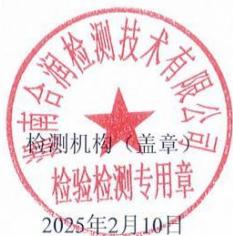
\includegraphics[width=0.85\linewidth]{images/c8ae8a040dcdca6d146634d818e1d0144ce9dfe31de7bc4a9cade54de380cbb2.jpg}
\end{figure}


签发日期：

审核人：

\begin{figure}[H]
\centering
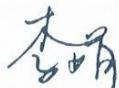
\includegraphics[width=0.85\linewidth]{images/dcf1ac8b7df08438d1f3c3a24a5e527007b24ee54305cd55873d1be69be9f0d8.jpg}
\end{figure}


\begin{figure}[H]
\centering
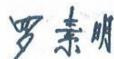
\includegraphics[width=0.85\linewidth]{images/6f643158cd38da92bd7006117522ee3ed8ea7905157fc7396ad866b66d731a13.jpg}
\end{figure}


\subsubsection{湖南合润检测技术有限公司}

\subsubsection{检测报告}

样品受理编号： 2404W0038


\begin{table}[H]
\centering
\begin{tabular}{|c|c|c|c|}
\hline
检测项目 & 个人剂量监测 & 检测方法 & 热释光检测法 \\
\hline
用人单位 & 萍乡市人民医院 & 委托单位 & 萍乡市人民医院 \\
\hline
检测/评价依据 & GBZ 128-2019 职业性外照射个人监测规范 & 检测日期 & 2025年1月22日 \\
\hline
检测室名称 & 个人剂量室 & 检测类别/目的 & 委托/常规监测 \\
\hline
检测仪器名称/型号/编号 & 热释光剂量仪/RGD-3D/SC1904019 & 探测器 & 热释光剂量计(TLD)-片状(圆片)-LiF(Mg,Cu,P) \\
\hline
\end{tabular}
\end{table}


检测结果：

\begin{table}[H]
\centering
\begin{tabular}{|c|c|c|c|c|c|c|c|}
\hline
编号 & 姓名 & 性别 & 职业类别 & 剂量计佩戴起止日期 & 个人剂量当量(mSv) &  &  \\
\hline
铅衣外( H\_\{p\}(10) ) & 铅衣内( H\_\{p\}(10) ) & 有效剂量( H\_\{p\}(10) ) &  &  &  &  &  \\
\hline
W0038001P & 邹南安 & 男 & 诊断放射学(2A) & 2024.10.1-2024.12.31 &  &  & 0.06 \\
\hline
W0038002P & 巫启恒 & 男 & 诊断放射学(2A) & 2024.10.1-2024.12.31 &  &  & 0.02* \\
\hline
W0038003P & 黎英 & 女 & 诊断放射学(2A) & 2024.10.1-2024.12.31 &  &  & 0.08 \\
\hline
W0038004P & 刘锋 & 男 & 诊断放射学(2A) & 2024.10.1-2024.12.31 &  &  & 0.09 \\
\hline
W0038005P & 刘小红 & 女 & 诊断放射学(2A) & 2024.10.1-2024.12.31 &  &  & 0.02* \\
\hline
W0038006P & 李丰章 & 男 & 诊断放射学(2A) & 2024.10.1-2024.12.31 &  &  & 0.02* \\
\hline
W0038007P & 黄元发 & 男 & 诊断放射学(2A) & 2024.10.1-2024.12.31 &  &  & 0.02* \\
\hline
W0038008P & 曾志宏 & 男 & 诊断放射学(2A) & 2024.10.1-2024.12.31 &  &  & 0.02* \\
\hline
W0038009P & 谭华 & 男 & 诊断放射学(2A) & 2024.10.1-2024.12.31 &  &  & 0.02* \\
\hline
W0038010P & 陈萍赣 & 男 & 诊断放射学(2A) & 2024.10.1-2024.12.31 &  &  & 0.08 \\
\hline
W0038011P & 郭欣 & 男 & 诊断放射学(2A) & 2024.10.1-2024.12.31 &  &  & 0.06 \\
\hline
W0038012P & 钟自华 & 男 & 诊断放射学(2A) & 2024.10.1-2024.12.31 &  &  & 0.02* \\
\hline
W0038013P & 陈洋勇 & 男 & 诊断放射学(2A) & 2024.10.1-2024.12.31 &  &  & 0.02* \\
\hline
W0038014P & 刘霞 & 女 & 诊断放射学(2A) & 2024.10.1-2024.12.31 &  &  & 0.02* \\
\hline
W0038015P & 陈亮 & 男 & 诊断放射学(2A) & 2024.10.1-2024.12.31 &  &  & 0.05 \\
\hline
\end{tabular}
\end{table}


检测结果：
共7页第2页

\begin{table}[H]
\centering
\begin{tabular}{|c|c|c|c|c|c|c|c|}
\hline
编号 & 姓名 & 性别 & 职业类别 & 剂量计佩戴起止日期 & 个人剂量当量(mSv) &  &  \\
\hline
铅衣外Hp(10) & 铅衣内Hp(10) & 有效剂量Hp(10) &  &  &  &  &  \\
\hline
W0038016P & 傅志颖 & 女 & 诊断放射学(2A) & 2024.10.1-2024.12.31 &  &  & 0.02* \\
\hline
W0038017P & 李琪 & 男 & 诊断放射学(2A) & 2024.10.1-2024.12.31 &  &  & 0.02* \\
\hline
W0038018P & 周晶 & 女 & 诊断放射学(2A) & 2024.10.1-2024.12.31 &  &  & 0.02* \\
\hline
W0038019P & 肖维国 & 男 & 诊断放射学(2A) & 2024.10.1-2024.12.31 &  &  & 0.27 \\
\hline
W0038020P & 刘天笑 & 女 & 诊断放射学(2A) & 2024.10.1-2024.12.31 &  &  & 0.02* \\
\hline
W0038021P & 王敬朋 & 男 & 诊断放射学(2A) & 2024.10.1-2024.12.31 &  &  & 0.04 \\
\hline
W0038022P & 王爱华 & 女 & 诊断放射学(2A) & 2024.10.1-2024.12.31 &  &  & 0.06 \\
\hline
W0038023P & 崔甜甜 & 女 & 诊断放射学(2A) & 2024.10.1-2024.12.31 &  &  & 0.02* \\
\hline
W0038024P & 杜红 & 女 & 诊断放射学(2A) & 2024.10.1-2024.12.31 &  &  & 0.02* \\
\hline
W0038025P & 文翠 & 女 & 诊断放射学(2A) & 2024.10.1-2024.12.31 &  &  & 0.02* \\
\hline
W0038026P & 易鑫 & 男 & 诊断放射学(2A) & 2024.10.1-2024.12.31 &  &  & 0.02* \\
\hline
W0038027P & 贺曦 & 男 & 诊断放射学(2A) & 2024.10.1-2024.12.31 &  &  & 0.02* \\
\hline
W0038028P & 万红 & 女 & 诊断放射学(2A) & 2024.10.1-2024.12.31 &  &  & 0.02* \\
\hline
W0038029P & 廖林 & 女 & 诊断放射学(2A) & 2024.10.1-2024.12.31 &  &  & 0.02* \\
\hline
W0038030P & 张晓玲 & 女 & 诊断放射学(2A) & 2024.10.1-2024.12.31 &  &  & 0.02* \\
\hline
W0038031P & 黎安琪 & 女 & 诊断放射学(2A) & 2024.10.1-2024.12.31 &  &  & 0.02* \\
\hline
W0038032P & 吴正波 & 男 & 诊断放射学(2A) & 2024.10.1-2024.12.31 &  &  & 0.02* \\
\hline
W0038033P & 王德华 & 男 & 诊断放射学(2A) & 2024.10.1-2024.12.31 &  &  & 0.02* \\
\hline
W0038034P & 吴斌 & 男 & 诊断放射学(2A) & 2024.10.1-2024.12.31 &  &  & 0.06 \\
\hline
W0038035P & 易阳 & 女 & 诊断放射学(2A) & 2024.10.1-2024.12.31 &  &  & 0.08 \\
\hline
W0038036P & 汤裕兵 & 男 & 诊断放射学(2A) & 2024.10.1-2024.12.31 &  &  & 0.02* \\
\hline
W0038037P & 黄瑶 & 女 & 诊断放射学(2A) & 2024.10.1-2024.12.31 &  &  & 0.02* \\
\hline
W0038038P & 雍好琴 & 女 & 诊断放射学(2A) & 2024.10.1-2024.12.31 &  &  & 0.07 \\
\hline
W0038039P & 杨迪 & 女 & 诊断放射学(2A) & 2024.10.1-2024.12.31 &  &  & 0.02* \\
\hline
W0038040P & 王敏 & 女 & 诊断放射学(2A) & 2024.10.1-2024.12.31 &  &  & 0.02* \\
\hline
W0038041P & 杨道益 & 男 & 诊断放射学(2A) & 2024.10.1-2024.12.31 &  &  & 0.02* \\
\hline
W0038042P & 沈雯婷 & 女 & 诊断放射学(2A) & 2024.10.1-2024.12.31 &  &  & 0.02* \\
\hline
W0038043P & 捷继斯 & 男 & 诊断放射学(2A) & 2024.10.1-2024.12.31 &  &  & 0.02* \\
\hline
\end{tabular}
\end{table}


检测结果：


\begin{table}[H]
\centering
\begin{tabular}{|c|c|c|c|c|c|c|c|}
\hline
编号 & 姓名 & 性别 & 职业类别 & 剂量计佩戴起止日期 & 个人剂量当量(mSv) &  &  \\
\hline
铅衣外Hp(10) & 铅衣内Hp(10) & 有效剂量Hp(10) &  &  &  &  &  \\
\hline
W0038044P & 龙安友 & 男 & 诊断放射学(2A) & 2024.10.1-2024.12.31 &  &  & 0.02* \\
\hline
W0038045P & 周宇煊 & 男 & 诊断放射学(2A) & 2024.10.1-2024.12.31 &  &  & 0.02* \\
\hline
W0038046P & 陈智勇 & 男 & 诊断放射学(2A) & 2024.10.1-2024.12.31 &  &  & 0.05 \\
\hline
W0038047P & 何婷 & 女 & 诊断放射学(2A) & 2024.10.1-2024.12.31 &  &  & 0.02* \\
\hline
W0038048P & 张崇海 & 男 & 诊断放射学(2A) & 2024.10.1-2024.12.31 &  &  & 0.02* \\
\hline
W0038049P & 黄紫娴 & 女 & 诊断放射学(2A) & 2024.10.1-2024.12.31 &  &  & 0.02* \\
\hline
W0038050P & 龙阳天利 & 女 & 诊断放射学(2A) & 2024.10.1-2024.12.31 &  &  & 0.02* \\
\hline
W0038051P & 李健 & 男 & 诊断放射学(2A) & 2024.10.1-2024.12.31 &  &  & 0.02* \\
\hline
W0038052P & 叶作增 & 男 & 诊断放射学(2A) & 2024.10.1-2024.12.31 &  &  & 0.02* \\
\hline
W0038053P & 周礼平 & 男 & 诊断放射学(2A) & 2024.10.1-2024.12.31 &  &  & 0.04 \\
\hline
W0038054P & 黄丽 & 女 & 诊断放射学(2A) & 2024.10.1-2024.12.31 &  &  & 0.02* \\
\hline
W0038055P & 靡洪 & 男 & 诊断放射学(2A) & 2024.10.1-2024.12.31 &  &  & 0.02* \\
\hline
W0038056P & 廖晓慧 & 女 & 诊断放射学(2A) & 2024.10.1-2024.12.31 &  &  & 0.02* \\
\hline
W0038057P & 邓莎 & 女 & 诊断放射学(2A) & 2024.10.1-2024.12.31 &  &  & 0.04 \\
\hline
W0038058P & 易江 & 男 & 诊断放射学(2A) & 2024.10.1-2024.12.31 &  &  & 0.02* \\
\hline
W0038059P & 彭向丽 & 女 & 诊断放射学(2A) & 2024.10.1-2024.12.31 &  &  & 0.02* \\
\hline
W0038060P & 唐志武 & 男 & 诊断放射学(2A) & 2024.10.1-2024.12.31 &  &  & 0.02* \\
\hline
W0038061P & 彭其 & - & 诊断放射学(2A) & 2024.10.1-2024.12.31 &  &  & 0.02* \\
\hline
W0038062P & 刘涛 & - & 诊断放射学(2A) & 2024.10.1-2024.12.31 &  &  & 0.04 \\
\hline
W0038063P & 廖延亮 & 男 & 诊断放射学(2A) & 2024.10.1-2024.12.31 &  &  & 0.10 \\
\hline
W0038064P & 蔡坤豪 & 男 & 诊断放射学(2A) & 2024.10.1-2024.12.31 &  &  & 0.02* \\
\hline
W0038065P & 欧阳公怒 & 男 & 其他应用(2F) & 2024.10.1-2024.12.31 &  &  & 0.02* \\
\hline
W0038066P & 陈明伟 & 男 & 放射治疗(2D) & 2024.10.1-2024.12.31 &  &  & 0.15 \\
\hline
W0038067P & 黄华堂 & 男 & 放射治疗(2D) & 2024.10.1-2024.12.31 &  &  & 0.08 \\
\hline
W0038068P & 张红宇 & 女 & 放射治疗(2D) & 2024.10.1-2024.12.31 &  &  & 0.02* \\
\hline
W0038069P & 辛焕中 & 男 & 放射治疗(2D) & 2024.10.1-2024.12.31 &  &  & 0.02* \\
\hline
W0038070P & 胡依冰 & 女 & 放射治疗(2D) & 2024.10.1-2024.12.31 &  &  & 0.02* \\
\hline
W0038071P & 刘鲁根 & 男 & 放射治疗(2D) & 2024.10.1-2024.12.31 &  &  & 0.06 \\
\hline
\end{tabular}
\end{table}


检测结果：
共7页第4页

\begin{table}[H]
\centering
\begin{tabular}{|c|c|c|c|c|c|c|c|}
\hline
编号 & 姓名 & 性别 & 职业类别 & 剂量计佩戴起止日期 & 个人剂量当量(mSv) &  &  \\
\hline
铅衣外Hp(10) & 铅衣内Hp(10) & 有效剂量Hp(10) &  &  &  &  &  \\
\hline
W0038072P & 乔浩 & 男 & 放射治疗(2D) & 2024.10.1-2024.12.31 &  &  & 0.05 \\
\hline
W0038073P & 黄珍 & 女 & 放射治疗(2D) & 2024.10.1-2024.12.31 &  &  & 0.02* \\
\hline
W0038074P & 李露 & 女 & 放射治疗(2D) & 2024.10.1-2024.12.31 &  &  & 0.53 \\
\hline
W0038075P & 周怡 & 女 & 放射治疗(2D) & 2024.10.1-2024.12.31 &  &  & 0.02* \\
\hline
W0038076K & 李鹏 & 男 & 核医学(2C) & 2024.10.1-2024.12.31 & 0.15 & 0.07 &  \\
\hline
W0038077K & 杨凭飞 & 男 & 核医学(2C) & 2024.10.1-2024.12.31 & 0.22 & 0.09 &  \\
\hline
W0038078K & 文晓琴 & 女 & 核医学(2C) & 2024.10.1-2024.12.31 & 0.14 & 0.02* &  \\
\hline
W0038079K & 黎心四 & 男 & 核医学(2C) & 2024.10.1-2024.12.31 & 0.27 & 0.11 &  \\
\hline
W0038080K & 张西 & 女 & 核医学(2C) & 2024.10.1-2024.12.31 & 0.20 & 0.08 &  \\
\hline
W0038081K & 王健 & 男 & 核医学(2C) & 2024.10.1-2024.12.31 & 0.18 & 0.05 &  \\
\hline
W0038082K & 任妹 & 女 & 核医学(2C) & 2024.10.1-2024.12.31 & 0.17 & 0.05 &  \\
\hline
W0038083K & 周慧 & 女 & 核医学(2C) & 2024.10.1-2024.12.31 & 0.13 & 0.10 &  \\
\hline
W0038084K & 陈娇 & 女 & 核医学(2C) & 2024.10.1-2024.12.31 & 0.19 & 0.06 &  \\
\hline
W0038085K & 许优 & 女 & 核医学(2C) & 2024.10.1-2024.12.31 & 0.20 & 0.09 &  \\
\hline
W0038086K & 董文哲 & 男 & 介入放射学(2E) & 2024.10.1-2024.12.31 & 0.38\# & 0.04\# &  \\
\hline
W0038087K & 肖江 & 女 & 介入放射学(2E) & 2024.10.1-2024.12.31 & 0.30 & 0.02* &  \\
\hline
W0038088K & 郑磊 & 男 & 介入放射学(2E) & 2024.10.1-2024.12.31 & 0.12 & 0.02* &  \\
\hline
W0038089K & 林婷 & 女 & 介入放射学(2E) & 2024.10.1-2024.12.31 & 0.22 & 0.02* &  \\
\hline
W0038090K & 周春春 & 女 & 介入放射学(2E) & 2024.10.1-2024.12.31 & 0.27 & 0.02* &  \\
\hline
W0038091K & 杨侃 & 男 & 介入放射学(2E) & 2024.10.1-2024.12.31 & 0.43 & 0.02* &  \\
\hline
W0038092K & 易瀚杰 & 男 & 介入放射学(2E) & 2024.10.1-2024.12.31 & 0.02* & 0.02*\# &  \\
\hline
W0038093K & 刘晨曦 & 女 & 介入放射学(2E) & 2024.10.1-2024.12.31 & 0.38\# & 0.04\# &  \\
\hline
W0038094K & 李苏琴 & 女 & 介入放射学(2E) & 2024.10.1-2024.12.31 & 0.83 & 0.02* &  \\
\hline
W0038095K & 刘建刚 & 男 & 介入放射学(2E) & 2024.10.1-2024.12.31 & 0.38\# & 0.04\# &  \\
\hline
W0038096K & 刘霞 & 女 & 介入放射学(2E) & 2024.10.1-2024.12.31 & 0.02* & 0.02* &  \\
\hline
W0038097K & 彭治鹏 & 男 & 介入放射学(2E) & 2024.10.1-2024.12.31 & 0.12 & 0.02* &  \\
\hline
W0038098K & 张涵茹 & 女 & 介入放射学(2E) & 2024.10.1-2024.12.31 & 0.09 & 0.02* &  \\
\hline
W0038099K & 朱敏 & 女 & 介入放射学(2E) & 2024.10.1-2024.12.31 & 0.38\# & 0.04\# &  \\
\hline
\end{tabular}
\end{table}


检测结果：
共7页第5页

\begin{table}[H]
\centering
\begin{tabular}{|c|c|c|c|c|c|c|c|}
\hline
编号 & 姓名 & 性别 & 职业类别 & 剂量计佩戴起止日期 & 个人剂量当量(mSv) &  &  \\
\hline
铅衣外Hp(10) & 铅衣内Hp(10) & 有效剂量Hp(10) &  &  &  &  &  \\
\hline
W0038100K & 韩涛 & 男 & 介入放射学(2E) & 2024.10.1-2024.12.31 & 0.38\# & 0.04\# &  \\
\hline
W0038101K & 廖骞 & 男 & 介入放射学(2E) & 2024.10.1-2024.12.31 & 0.16 & 0.02* &  \\
\hline
W0038102K & 蔡恒烈 & 男 & 介入放射学(2E) & 2024.10.1-2024.12.31 & 0.09 & 0.02* &  \\
\hline
W0038103K & 王奕 & 男 & 介入放射学(2E) & 2024.10.1-2024.12.31 & 0.10 & 0.02* &  \\
\hline
W0038104K & 张志强 & 男 & 介入放射学(2E) & 2024.10.1-2024.12.31 & 0.35 & 0.18 &  \\
\hline
W0038105K & 崔钢 & 男 & 介入放射学(2E) & 2024.10.1-2024.12.31 & 0.08 & 0.02* &  \\
\hline
W0038106K & 严兵 & 男 & 介入放射学(2E) & 2024.10.1-2024.12.31 & 0.38\# & 0.04\# &  \\
\hline
W0038107K & 龚敏 & 男 & 介入放射学(2E) & 2024.10.1-2024.12.31 & 0.12 & 0.02* &  \\
\hline
W0038108K & 韩明 & 男 & 介入放射学(2E) & 2024.10.1-2024.12.31 & 0.09 & 0.02* &  \\
\hline
W0038109K & 邱萍 & 男 & 介入放射学(2E) & 2024.10.1-2024.12.31 & 0.14 & 0.02* &  \\
\hline
W0038110K & 贺娇 & 女 & 介入放射学(2E) & 2024.10.1-2024.12.31 & 0.09 & 0.02* &  \\
\hline
W0038111K & 付云辉 & 男 & 介入放射学(2E) & 2024.10.1-2024.12.31 & 0.07 & 0.02* &  \\
\hline
W0038112K & 吴朝 & 男 & 介入放射学(2E) & 2024.10.1-2024.12.31 & 0.10 & 0.02* &  \\
\hline
W0038113K & 郑旺 & 男 & 介入放射学(2E) & 2024.10.1-2024.12.31 & 0.10 & 0.02* &  \\
\hline
W0038114K & 兰前鑫 & 男 & 介入放射学(2E) & 2024.10.1-2024.12.31 & 0.06 & 0.02* &  \\
\hline
W0038115K & 朱勇美 & 女 & 介入放射学(2E) & 2024.10.1-2024.12.31 & 0.16 & 0.02* &  \\
\hline
W0038116K & 黄文军 & 男 & 介入放射学(2E) & 2024.10.1-2024.12.31 & 0.04 & 0.02* &  \\
\hline
W0038117K & 周国忠 & 男 & 介入放射学(2E) & 2024.10.1-2024.12.31 & 2.57 & 0.09 &  \\
\hline
W0038118K & 罗勤 & 男 & 介入放射学(2E) & 2024.10.1-2024.12.31 & 2.85 & 0.02*\# &  \\
\hline
W0038119K & 姚常 & 男 & 介入放射学(2E) & 2024.10.1-2024.12.31 & 3.09 & 0.02*\# &  \\
\hline
W0038120K & 彭阳 & 男 & 介入放射学(2E) & 2024.10.1-2024.12.31 & 0.10 & 0.02* &  \\
\hline
W0038121K & 刘兴龙 & 男 & 介入放射学(2E) & 2024.10.1-2024.12.31 & 0.23 & 0.05 &  \\
\hline
W0038122K & 周吕桢 & 男 & 介入放射学(2E) & 2024.10.1-2024.12.31 & 0.04 & 0.02* &  \\
\hline
W0038123K & 陈小根 & - & 介入放射学(2E) & 2024.10.1-2024.12.31 & 0.72 & 0.09 &  \\
\hline
W0038124K & 闫博宇 & 男 & 介入放射学(2E) & 2024.10.1-2024.12.31 & 0.38\# & 0.04\# &  \\
\hline
W0038125K & 张学洪 & 男 & 介入放射学(2E) & 2024.10.1-2024.12.31 & 0.04 & 0.02* &  \\
\hline
W0038126K & 张雨虹 & 男 & 介入放射学(2E) & 2024.10.1-2024.12.31 & 0.15 & 0.02* &  \\
\hline
W0038127K & 曾广忠 & 男 & 介入放射学(2E) & 2024.10.1-2024.12.31 & 0.24\# & 0.02*\# &  \\
\hline
\end{tabular}
\end{table}


检测结果：
共7页第6页

\begin{table}[H]
\centering
\begin{tabular}{|c|c|c|c|c|c|c|c|}
\hline
编号 & 姓名 & 性别 & 职业类别 & 剂量计佩戴起止日期 & 个人剂量当量(mSv) &  &  \\
\hline
铅衣外Hp(10) & 铅衣内Hp(10) & 有效剂量Hp(10) &  &  &  &  &  \\
\hline
W0038128K & 邱明涛 & 男 & 介入放射学(2E) & 2024.10.1-2024.12.31 & 0.24\# & 0.02*\# &  \\
\hline
W0038129K & 邓海明 & 男 & 介入放射学(2E) & 2024.10.1-2024.12.31 & 0.05 & 0.02* &  \\
\hline
W0038130K & 邱建 & 男 & 介入放射学(2E) & 2024.10.1-2024.12.31 & 0.08 & 0.02* &  \\
\hline
W0038131K & 李晨 & 男 & 介入放射学(2E) & 2024.10.1-2024.12.31 & 0.69 & 0.02*\# &  \\
\hline
W0038132K & 赖丹 & 男 & 介入放射学(2E) & 2024.10.1-2024.12.31 & 0.04 & 0.02* &  \\
\hline
W0038133K & 毛云飞 & 男 & 介入放射学(2E) & 2024.10.1-2024.12.31 & 0.47 & 0.02* &  \\
\hline
W0038134K & 刘帅 & 男 & 介入放射学(2E) & 2024.10.1-2024.12.31 & 0.09 & 0.02* &  \\
\hline
W0038135K & 胡斌 & 男 & 介入放射学(2E) & 2024.10.1-2024.12.31 & 0.15 & 0.02* &  \\
\hline
W0038136K & 彭成福 & 男 & 介入放射学(2E) & 2024.10.1-2024.12.31 & 0.85 & 0.17 &  \\
\hline
W0038137K & 李洛 & 男 & 介入放射学(2E) & 2024.10.1-2024.12.31 & 1.13 & 0.04 &  \\
\hline
W0038138K & 朱飞 & 男 & 介入放射学(2E) & 2024.10.1-2024.12.31 & 1.78 & 0.16 &  \\
\hline
W0038139K & 丁绍纯 & 男 & 介入放射学(2E) & 2024.10.1-2024.12.31 & 0.95 & 0.73 &  \\
\hline
W0038140K & 王稻 & 男 & 介入放射学(2E) & 2024.10.1-2024.12.31 & 0.02* & 0.02* &  \\
\hline
W0038141K & 刘灏灏 & 男 & 介入放射学(2E) & 2024.10.1-2024.12.31 & 0.04 & 0.02* &  \\
\hline
W0038142K & 孙芬芬 & 女 & 介入放射学(2E) & 2024.10.1-2024.12.31 & 0.07 & 0.02* &  \\
\hline
W0038143K & 王俊东 & 男 & 介入放射学(2E) & 2024.10.1-2024.12.31 & 0.10 & 0.02* &  \\
\hline
W0038144K & 廖鹏 & 男 & 介入放射学(2E) & 2024.10.1-2024.12.31 & 0.09 & 0.02* &  \\
\hline
W0038145K & 贺小张 & 男 & 介入放射学(2E) & 2024.10.1-2024.12.31 & 0.02* & 0.02* &  \\
\hline
W0038146K & 许绍林 & 男 & 介入放射学(2E) & 2024.10.1-2024.12.31 & 0.05 & 0.02* &  \\
\hline
W0038147K & 余凯龙 & 男 & 介入放射学(2E) & 2024.10.1-2024.12.31 & 0.13 & 0.02* &  \\
\hline
W0038148K & 胡芯源 & 男 & 介入放射学(2E) & 2024.10.1-2024.12.31 & 0.02* & 0.02* &  \\
\hline
W0038149K & 王长庚 & 男 & 介入放射学(2E) & 2024.10.1-2024.12.31 & 0.32 & 0.02* &  \\
\hline
W0038150K & 杨德猛 & 男 & 介入放射学(2E) & 2024.10.1-2024.12.31 & 1.30 & 0.02* &  \\
\hline
W0038151K & 姜一帆 & 男 & 介入放射学(2E) & 2024.10.1-2024.12.31 & 0.38\# & 0.04\# &  \\
\hline
W0038152K & 胡小辉 & 男 & 介入放射学(2E) & 2024.10.1-2024.12.31 & 0.22 & 0.02* &  \\
\hline
W0038153K & 曹世超 & 男 & 介入放射学(2E) & 2024.10.1-2024.12.31 & 1.14 & 0.02* &  \\
\hline
W0038154K & 徐辉 & 男 & 介入放射学(2E) & 2024.10.1-2024.12.31 & 0.05 & 0.02* &  \\
\hline
W0038155K & 漆招 & 男 & 介入放射学(2E) & 2024.10.1-2024.12.31 & 0.08 & 0.02* &  \\
\hline
\end{tabular}
\end{table}


检测结果：
共7页第7页

\begin{table}[H]
\centering
\begin{tabular}{|c|c|c|c|c|c|c|c|}
\hline
编号 & 姓名 & 性别 & 职业类别 & 剂量计佩戴起止日期 & 个人剂量当量(mSv) &  &  \\
\hline
铅衣外Hp(10) & 铅衣内Hp(10) & 有效剂量Hp(10) &  &  &  &  &  \\
\hline
W0038156K & 巫志国 & 男 & 介入放射学(2E) & 2024.10.1-2024.12.31 & 0.02* & 0.02* &  \\
\hline
W0038157K & 柳毅 & 男 & 介入放射学(2E) & 2024.10.1-2024.12.31 & 0.02* & 0.02* &  \\
\hline
W0038158K & 沈婕 & 女 & 介入放射学(2E) & 2024.10.1-2024.12.31 & 0.06 & 0.02* &  \\
\hline
W0038159K & 刘可可 & 女 & 介入放射学(2E) & 2024.10.1-2024.12.31 & 0.04 & 0.02* &  \\
\hline
(以下空白) &  &  &  &  &  &  &  \\
\hline
\end{tabular}
\end{table}


\begin{figure}[H]
\centering

\includegraphics[width=0.85\linewidth]{images/1e2e70bb491918998b29e670294ee1a08c65adb8bedd19d7379f91850b31d0ac.jpg}
\end{figure}


\subsubsection{湖南合润检测技术有限公司}

\subsubsection{HUNAN HERUN TESTING TECHNOLOGY CO.LTD}

\begin{figure}[H]
\centering

\includegraphics[width=0.85\linewidth]{images/22085c3faad644d27ff130c6621a4146d301f9c0009273917e1bd0af7d62a530.jpg}
\end{figure}


211803102214

\subsubsection{检测报告}

\subsubsection{TEST REPORT}

报告编号：

ReportNo.

25HRJLW0038Q01

检测项目：

Test items

X/y射线外照射个人剂量监测Hp(10)

检测类型：

Detection type

委托监测/常规监测

委托单位：

Client

萍乡市人民医院

样品名称：

Sample name

\begin{figure}[H]
\centering
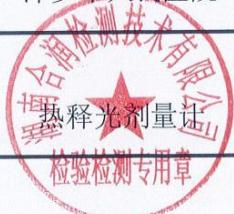
\includegraphics[width=0.85\linewidth]{images/12a059d17f23d7714b36db78f41e229976c945019a0fbb176840fe1695a5faea.jpg}
\end{figure}


报告日期：

Date of Report

2025年5月12日

检测单位：湖南合润检测技术有限公司

电话：0731-85058578

传真：0731-85058578

\subsubsection{注意事项}

\subsubsection{CONSIDERATIONS}

1.本报告无检验检测机构“检测报告专用章”无效。
2.本报告无“CMA”标志不具备法律证明作用。
3.复制本报告未重新加盖“检测报告专用章”无效。
4.本报告无报告签发人（授权签字人）签名无效。
5.本报告涂改无效。


8.本报告解释权归检验检测单位。

准确满意的服务；
与任何有损于检验检测判断的独立性和诚信度的活动；绝不参与和检验检测项目或者类似的竞争性项目有

\subsubsection{检测报告}

\subsubsection{REPORT OFTEST}

报告编号：

25HRJLW0038Q01

委托单位：

萍乡市人民医院

ReportNo.

Client

1.本次监测的主要技术依据(Referencedocuments forthe test)：

《职业性外照射个人监测监测规范》（GBZ128—2019）

《电离辐射防护与放射源安全基本标准》（GB18871—2002）

2.本次监测的环境条件(Environmentconditionforthetest)：

室内温度：

室内湿度：

\%RH

3.本次监测所使用的主要测量设备(Main standardsofmeasurementused inthe test)：

证书号/有效期

溯源机构

Description/Model

Serial No.

Certificate No./Due Date

Traceability Institute

热释光剂量仪/RGD-3D

SC1904019

2024H21-20- 5449245001/2025.9.3

上海市计量测试技术研究院/华东国家计量测试中心

\begin{figure}[H]
\centering
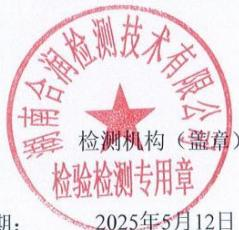
\includegraphics[width=0.85\linewidth]{images/35d2ae76122d3a51065c0b774da9af896ba0863f73f5ae0b903656570b5d6db4.jpg}
\end{figure}


审核人：

\subsubsection{湖南合润检测技术有限公司}

\subsubsection{检测报告}

\begin{table}[H]
\centering
\begin{tabular}{|c|c|c|c|}
\hline
样品受理编号: 2501W0038 共7页 第1页 &  &  &  \\
\hline
检测项目 & 个人剂量监测 & 检测方法 & 热释光检测法 \\
\hline
用人单位 & 萍乡市人民医院 & 委托单位 & 萍乡市人民医院 \\
\hline
检测/评价依据 & GBZ 128-2019 职业性外照射个人监测规范 & 检测日期 & 2025年4月22日 \\
\hline
检测室名称 & 个人剂量室 & 检测类别/目的 & 委托/常规监测 \\
\hline
检测仪器名称/型号/编号 & 热释光剂量仪/RGD-3D/SC1904019 & 探测器 & 热释光剂量计(TLD)-片状(圆片)-LiF(Mg,Cu,P) \\
\hline
\end{tabular}
\end{table}


检测结果：

\begin{table}[H]
\centering
\begin{tabular}{|c|c|c|c|c|c|c|c|}
\hline
编号 & 姓名 & 性别 & 职业类别 & 剂量计佩戴起止日期 & 个人剂量当量 (mSv) &  &  \\
\hline
铅衣外( H\_\{p\}(10) ) & 铅衣内( H\_\{p\}(10) ) & 有效剂量( H\_\{p\}(10) ) &  &  &  &  &  \\
\hline
W0038001P & 邹南安 & 男 & 诊断放射学(2A) & 2025.1.1-2025.3.31 &  &  & 0.08 \\
\hline
W0038002P & 巫启恒 & 男 & 诊断放射学(2A) & 2025.1.1-2025.3.31 &  &  & 0.02* \\
\hline
W0038003P & 黎英 & 女 & 诊断放射学(2A) & 2025.1.1-2025.3.31 &  &  & 0.02* \\
\hline
W0038004P & 刘锋 & 男 & 诊断放射学(2A) & 2025.1.1-2025.3.31 &  &  & 0.02* \\
\hline
W0038005P & 刘小红 & 女 & 诊断放射学(2A) & 2025.1.1-2025.3.31 &  &  & 0.02* \\
\hline
W0038006P & 李丰章 & 男 & 诊断放射学(2A) & 2025.1.1-2025.3.31 &  &  & 0.02* \\
\hline
W0038007P & 黄元发 & 男 & 诊断放射学(2A) & 2025.1.1-2025.3.31 &  &  & 0.02* \\
\hline
W0038008P & 曾志宏 & 男 & 诊断放射学(2A) & 2025.1.1-2025.3.31 &  &  & 0.02* \\
\hline
W0038009P & 谭华 & 男 & 诊断放射学(2A) & 2025.1.1-2025.3.31 &  &  & 0.02\# \\
\hline
W0038010P & 陈萍赣 & 男 & 诊断放射学(2A) & 2025.1.1-2025.3.31 &  &  & 0.02* \\
\hline
W0038011P & 郭欣 & 男 & 诊断放射学(2A) & 2025.1.1-2025.3.31 &  &  & 0.04 \\
\hline
W0038012P & 钟自华 & 男 & 诊断放射学(2A) & 2025.1.1-2025.3.31 &  &  & 0.02* \\
\hline
W0038013P & 陈洋勇 & 男 & 诊断放射学(2A) & 2025.1.1-2025.3.31 &  &  & 0.02* \\
\hline
W0038014P & 刘霞 & 女 & 诊断放射学(2A) & 2025.1.1-2025.3.31 &  &  & 0.02* \\
\hline
W0038015P & 陈亮 & 男 & 诊断放射学(2A) & 2025.1.1-2025.3.31 &  &  & 0.02* \\
\hline
\end{tabular}
\end{table}


检测结果：


\begin{table}[H]
\centering
\begin{tabular}{|c|c|c|c|c|c|c|c|}
\hline
编号 & 姓名 & 性别 & 职业类别 & 剂量计佩戴起止日期 & 个人剂量当量(mSv) &  &  \\
\hline
铅衣外 & 铅衣内 & 有效剂量 &  &  &  &  &  \\
\hline
Hp(10) & Hp(10) & Hp(10) &  &  &  &  &  \\
\hline
W0038016P & 傅志颖 & 女 & 诊断放射学(2A) & 2025.1.1-2025.3.31 &  &  & 0.02* \\
\hline
W0038017P & 李琪 & 男 & 诊断放射学(2A) & 2025.1.1-2025.3.31 &  &  & 0.02\# \\
\hline
W0038018P & 周晶 & 女 & 诊断放射学(2A) & 2025.1.1-2025.3.31 &  &  & 0.02* \\
\hline
W0038019P & 肖维国 & 男 & 诊断放射学(2A) & 2025.1.1-2025.3.31 &  &  & 0.02* \\
\hline
W0038020P & 刘天笑 & 女 & 诊断放射学(2A) & 2025.1.1-2025.3.31 &  &  & 0.02* \\
\hline
W0038021P & 王敬朋 & 男 & 诊断放射学(2A) & 2025.1.1-2025.3.31 &  &  & 0.03 \\
\hline
W0038022P & 王爱华 & 女 & 诊断放射学(2A) & 2025.1.1-2025.3.31 &  &  & 0.05 \\
\hline
W0038023P & 崔甜甜 & 女 & 诊断放射学(2A) & 2025.1.1-2025.3.31 &  &  & 0.02* \\
\hline
W0038024P & 杜红 & 女 & 诊断放射学(2A) & 2025.1.1-2025.3.31 &  &  & 0.02* \\
\hline
W0038025P & 文翠 & 女 & 诊断放射学(2A) & 2025.1.1-2025.3.31 &  &  & 0.02* \\
\hline
W0038026P & 易鑫 & 男 & 诊断放射学(2A) & 2025.1.1-2025.3.31 &  &  & 0.02* \\
\hline
W0038027P & 贺曦 & 男 & 诊断放射学(2A) & 2025.1.1-2025.3.31 &  &  & 0.02* \\
\hline
W0038028P & 万红 & 女 & 诊断放射学(2A) & 2025.1.1-2025.3.31 &  &  & 0.02* \\
\hline
W0038029P & 廖林 & 女 & 诊断放射学(2A) & 2025.1.1-2025.3.31 &  &  & 0.02* \\
\hline
W0038030P & 张晓玲 & 女 & 诊断放射学(2A) & 2025.1.1-2025.3.31 &  &  & 0.02* \\
\hline
W0038031P & 黎安琪 & 女 & 诊断放射学(2A) & 2025.1.1-2025.3.31 &  &  & 0.02* \\
\hline
W0038032P & 吴正波 & 男 & 诊断放射学(2A) & 2025.1.1-2025.3.31 &  &  & 0.02* \\
\hline
W0038033P & 王德华 & 男 & 诊断放射学(2A) & 2025.1.1-2025.3.31 &  &  & 0.02* \\
\hline
W0038034P & 吴斌 & 男 & 诊断放射学(2A) & 2025.1.1-2025.3.31 &  &  & 0.02* \\
\hline
W0038035P & 易阳 & 女 & 诊断放射学(2A) & 2025.1.1-2025.3.31 &  &  & 0.02* \\
\hline
W0038036P & 汤裕兵 & 男 & 诊断放射学(2A) & 2025.1.1-2025.3.31 &  &  & 0.02* \\
\hline
W0038037P & 黄瑶 & 女 & 诊断放射学(2A) & 2025.1.1-2025.3.31 &  &  & 0.02* \\
\hline
W0038038P & 雍好琴 & 女 & 诊断放射学(2A) & 2025.1.1-2025.3.31 &  &  & 0.02* \\
\hline
W0038039P & 杨迪 & 女 & 诊断放射学(2A) & 2025.1.1-2025.3.31 &  &  & 0.02* \\
\hline
W0038040P & 王敏 & 女 & 诊断放射学(2A) & 2025.1.1-2025.3.31 &  &  & 0.02* \\
\hline
W0038041P & 杨道益 & 男 & 诊断放射学(2A) & 2025.1.1-2025.3.31 &  &  & 0.02* \\
\hline
W0038042P & 沈雯婷 & 女 & 诊断放射学(2A) & 2025.1.1-2025.3.31 &  &  & 0.02* \\
\hline
W0038043P & 捷继斯 & 男 & 诊断放射学(2A) & 2025.1.1-2025.3.31 &  &  & 0.02* \\
\hline
\end{tabular}
\end{table}


检测结果：
共7页第3页

\begin{table}[H]
\centering
\begin{tabular}{|c|c|c|c|c|c|c|c|}
\hline
编号 & 姓名 & 性别 & 职业类别 & 剂量计佩戴起止日期 & 个人剂量当量(mSv) &  &  \\
\hline
铅衣外Hp(10) & 铅衣内Hp(10) & 有效剂量Hp(10) &  &  &  &  &  \\
\hline
W0038044P & 龙安友 & 男 & 诊断放射学(2A) & 2025.1.1-2025.3.31 &  &  & 0.02* \\
\hline
W0038045P & 周宇煊 & 男 & 诊断放射学(2A) & 2025.1.1-2025.3.31 &  &  & 0.02* \\
\hline
W0038046P & 陈智勇 & 男 & 诊断放射学(2A) & 2025.1.1-2025.3.31 &  &  & 0.02* \\
\hline
W0038047P & 何婷 & 女 & 诊断放射学(2A) & 2025.1.1-2025.3.31 &  &  & 0.02* \\
\hline
W0038048P & 张崇海 & 男 & 诊断放射学(2A) & 2025.1.1-2025.3.31 &  &  & 0.02* \\
\hline
W0038049P & 黄紫娴 & 女 & 诊断放射学(2A) & 2025.1.1-2025.3.31 &  &  & 0.02* \\
\hline
W0038050P & 龙阳天利 & 女 & 诊断放射学(2A) & 2025.1.1-2025.3.31 &  &  & 0.02* \\
\hline
W0038051P & 李健 & 男 & 诊断放射学(2A) & 2025.1.1-2025.3.31 &  &  & 0.02* \\
\hline
W0038052P & 叶作增 & 男 & 诊断放射学(2A) & 2025.1.1-2025.3.31 &  &  & 0.02* \\
\hline
W0038053P & 周礼平 & 男 & 诊断放射学(2A) & 2025.1.1-2025.3.31 &  &  & 0.02* \\
\hline
W0038054P & 黄丽 & 女 & 诊断放射学(2A) & 2025.1.1-2025.3.31 &  &  & 0.02* \\
\hline
W0038055P & 靡洪 & 男 & 诊断放射学(2A) & 2025.1.1-2025.3.31 &  &  & 0.02* \\
\hline
W0038056P & 廖晓慧 & 女 & 诊断放射学(2A) & 2025.1.1-2025.3.31 &  &  & 0.02* \\
\hline
W0038057P & 邓莎 & 女 & 诊断放射学(2A) & 2025.1.1-2025.3.31 &  &  & 0.02* \\
\hline
W0038058P & 易江 & 男 & 诊断放射学(2A) & 2025.1.1-2025.3.31 &  &  & 0.02* \\
\hline
W0038059P & 彭向丽 & 女 & 诊断放射学(2A) & 2025.1.1-2025.3.31 &  &  & 0.02* \\
\hline
W0038060P & 唐志武 & 男 & 诊断放射学(2A) & 2025.1.1-2025.3.31 &  &  & 0.02* \\
\hline
W0038061P & 彭其 & - & 诊断放射学(2A) & 2025.1.1-2025.3.31 &  &  & 0.02* \\
\hline
W0038062P & 刘涛 & - & 诊断放射学(2A) & 2025.1.1-2025.3.31 &  &  & 0.02* \\
\hline
W0038063P & 廖延亮 & 男 & 诊断放射学(2A) & 2025.1.1-2025.3.31 &  &  & 0.03 \\
\hline
W0038160P & 胡笑东 & 男 & 诊断放射学(2A) & 2025.1.1-2025.3.31 &  &  & 0.02* \\
\hline
W0038161P & 彭进和 & 男 & 诊断放射学(2A) & 2025.1.1-2025.3.31 &  &  & 0.02* \\
\hline
W0038162P & 孙齐乐 & 男 & 诊断放射学(2A) & 2025.1.1-2025.3.31 &  &  & 0.02* \\
\hline
W0038163P & 文望东 & 女 & 诊断放射学(2A) & 2025.1.1-2025.3.31 &  &  & 0.02* \\
\hline
W0038164P & 蔡贺 & 男 & 诊断放射学(2A) & 2025.1.1-2025.3.31 &  &  & 0.02* \\
\hline
W0038064P & 蔡坤豪 & 男 & 诊断放射学(2A) & 2025.1.1-2025.3.31 &  &  & 0.02* \\
\hline
W0038065P & 欧阳公怒 & 男 & 其他应用(2F) & 2025.1.1-2025.3.31 &  &  & 0.02* \\
\hline
W0038066P & 陈明伟 & 男 & 放射治疗(2D) & 2025.1.1-2025.3.31 &  &  & 0.02* \\
\hline
\end{tabular}
\end{table}


检测结果：
共7页第4页

\begin{table}[H]
\centering
\begin{tabular}{|c|c|c|c|c|c|c|c|}
\hline
编号 & 姓名 & 性别 & 职业类别 & 剂量计佩戴起止日期 & 个人剂量当量(mSv) &  &  \\
\hline
铅衣外 & 铅衣内 & 有效剂量 &  &  &  &  &  \\
\hline
Hp(10) & Hp(10) & Hp(10) &  &  &  &  &  \\
\hline
W0038067P & 黄华堂 & 男 & 放射治疗(2D) & 2025.1.1-2025.3.31 &  &  & 0.02* \\
\hline
W0038068P & 张红宇 & 女 & 放射治疗(2D) & 2025.1.1-2025.3.31 &  &  & 0.02* \\
\hline
W0038069P & 辛焕中 & 男 & 放射治疗(2D) & 2025.1.1-2025.3.31 &  &  & 0.02* \\
\hline
W0038070P & 胡依冰 & 女 & 放射治疗(2D) & 2025.1.1-2025.3.31 &  &  & 0.02* \\
\hline
W0038071P & 刘鲁根 & 男 & 放射治疗(2D) & 2025.1.1-2025.3.31 &  &  & 0.02* \\
\hline
W0038072P & 乔浩 & 男 & 放射治疗(2D) & 2025.1.1-2025.3.31 &  &  & 0.02* \\
\hline
W0038073P & 黄珍 & 女 & 放射治疗(2D) & 2025.1.1-2025.3.31 &  &  & 0.02* \\
\hline
W0038074P & 李露 & 女 & 牙科放射学(2B) & 2025.1.1-2025.3.31 &  &  & 0.34 \\
\hline
W0038075P & 周怡 & 女 & 牙科放射学(2B) & 2025.1.1-2025.3.31 &  &  & 0.02* \\
\hline
W0038076K & 李鹏 & 男 & 核医学(2C) & 2025.1.1-2025.3.31 & 0.02* & 0.02* & 0.02* \\
\hline
W0038077K & 杨凭飞 & 男 & 核医学(2C) & 2025.1.1-2025.3.31 & 0.03 & 0.02* & 0.02* \\
\hline
W0038078K & 文晓琴 & 女 & 核医学(2C) & 2025.1.1-2025.3.31 & 0.03 & 0.02* & 0.02* \\
\hline
W0038079K & 黎心四 & 男 & 核医学(2C) & 2025.1.1-2025.3.31 & 0.05 & 0.03 & 0.02* \\
\hline
W0038080K & 张西 & 女 & 核医学(2C) & 2025.1.1-2025.3.31 & 0.05 & 0.02* & 0.02* \\
\hline
W0038081K & 王健 & 男 & 核医学(2C) & 2025.1.1-2025.3.31 & 0.07 & 0.02* & 0.02* \\
\hline
W0038082K & 任妹 & 女 & 核医学(2C) & 2025.1.1-2025.3.31 & 0.07 & 0.02* & 0.02* \\
\hline
W0038083K & 周慧 & 女 & 核医学(2C) & 2025.1.1-2025.3.31 & 0.03 & 0.02* & 0.02* \\
\hline
W0038084K & 陈娇 & 女 & 核医学(2C) & 2025.1.1-2025.3.31 & 0.05 & 0.04 & 0.02* \\
\hline
W0038085K & 许优 & 女 & 核医学(2C) & 2025.1.1-2025.3.31 & 0.02* & 0.02* & 0.02* \\
\hline
W0038086K & 董文哲 & 男 & 介入放射学(2E) & 2025.1.1-2025.3.31 & 0.02* & 0.02* & 0.02* \\
\hline
W0038087K & 肖江 & 女 & 介入放射学(2E) & 2025.1.1-2025.3.31 & 0.02* & 0.02* & 0.02* \\
\hline
W0038088K & 郑磊 & 男 & 介入放射学(2E) & 2025.1.1-2025.3.31 & 0.02* & 0.02* & 0.02* \\
\hline
W0038089K & 林婷 & 女 & 介入放射学(2E) & 2025.1.1-2025.3.31 & 0.02* & 0.02* & 0.02* \\
\hline
W0038090K & 周春春 & 女 & 介入放射学(2E) & 2025.1.1-2025.3.31 & 0.15 & 0.02* & 0.02* \\
\hline
W0038091K & 杨侃 & 男 & 介入放射学(2E) & 2025.1.1-2025.3.31 & 0.17 & 0.02* & 0.02* \\
\hline
W0038092K & 易瀚杰 & 男 & 介入放射学(2E) & 2025.1.1-2025.3.31 & 0.02* & 0.02* & 0.02* \\
\hline
W0038093K & 刘晨曦 & 女 & 介入放射学(2E) & 2025.1.1-2025.3.31 & 0.05\# & 0.02\# & 0.02\# \\
\hline
W0038094K & 李苏琴 & 女 & 介入放射学(2E) & 2025.1.1-2025.3.31 & 0.22 & 0.02* & 0.02* \\
\hline
\end{tabular}
\end{table}


检测结果：
共7页第5页

\begin{table}[H]
\centering
\begin{tabular}{|c|c|c|c|c|c|c|c|}
\hline
编号 & 姓名 & 性别 & 职业类别 & 剂量计佩戴起止日期 & 个人剂量当量(mSv) &  &  \\
\hline
铅衣外Hp(10) & 铅衣内Hp(10) & 有效剂量Hp(10) &  &  &  &  &  \\
\hline
W0038095K & 刘建刚 & 男 & 介入放射学(2E) & 2025.1.1-2025.3.31 & 0.02* & 0.02* & 0.02* \\
\hline
W0038096K & 刘霞 & 女 & 介入放射学(2E) & 2025.1.1-2025.3.31 & 0.02* & 0.02* & 0.02* \\
\hline
W0038097K & 彭治鹏 & 男 & 介入放射学(2E) & 2025.1.1-2025.3.31 & 0.02* & 0.02* & 0.02* \\
\hline
W0038098K & 张涵茹 & 女 & 介入放射学(2E) & 2025.1.1-2025.3.31 & 0.02* & 0.02* & 0.02* \\
\hline
W0038099K & 朱敏 & 女 & 介入放射学(2E) & 2025.1.1-2025.3.31 & 0.02* & 0.02* & 0.02* \\
\hline
W0038100K & 韩涛 & 男 & 介入放射学(2E) & 2025.1.1-2025.3.31 & 5.24 & 0.27 & 0.48 \\
\hline
W0038101K & 廖骞 & 男 & 介入放射学(2E) & 2025.1.1-2025.3.31 & 0.02* & 0.02* & 0.02* \\
\hline
W0038102K & 蔡恒烈 & 男 & 介入放射学(2E) & 2025.1.1-2025.3.31 & 0.05\# & 0.02\# & 0.02\# \\
\hline
W0038103K & 王奕 & 男 & 介入放射学(2E) & 2025.1.1-2025.3.31 & 0.02* & 0.02* & 0.02* \\
\hline
W0038104K & 张志强 & 男 & 介入放射学(2E) & 2025.1.1-2025.3.31 & 2.24 & 0.84 & 0.78 \\
\hline
W0038105K & 崔钢 & 男 & 介入放射学(2E) & 2025.1.1-2025.3.31 & 1.28\# & 0.20\# & 0.22\# \\
\hline
W0038106K & 严兵 & 男 & 介入放射学(2E) & 2025.1.1-2025.3.31 & 0.10 & 0.02* & 0.02* \\
\hline
W0038107K & 龚敏 & 男 & 介入放射学(2E) & 2025.1.1-2025.3.31 & 0.02* & 0.02* & 0.02* \\
\hline
W0038108K & 韩明 & 男 & 介入放射学(2E) & 2025.1.1-2025.3.31 & 0.02* & 0.02* & 0.02* \\
\hline
W0038109K & 邱萍 & 男 & 介入放射学(2E) & 2025.1.1-2025.3.31 & 0.02* & 0.02* & 0.02* \\
\hline
W0038110K & 贺娇 & 女 & 介入放射学(2E) & 2025.1.1-2025.3.31 & 0.02* & 0.02* & 0.02* \\
\hline
W0038111K & 付云辉 & 男 & 介入放射学(2E) & 2025.1.1-2025.3.31 & 0.02* & 0.02* & 0.02* \\
\hline
W0038112K & 吴朝 & 男 & 介入放射学(2E) & 2025.1.1-2025.3.31 & 0.02* & 0.02* & 0.02* \\
\hline
W0038113K & 郑旺 & 男 & 介入放射学(2E) & 2025.1.1-2025.3.31 & 0.02* & 0.02* & 0.02* \\
\hline
W0038114K & 兰前鑫 & 男 & 介入放射学(2E) & 2025.1.1-2025.3.31 & 0.02* & 0.02* & 0.02* \\
\hline
W0038115K & 朱勇美 & 女 & 介入放射学(2E) & 2025.1.1-2025.3.31 & 0.02* & 0.02* & 0.02* \\
\hline
W0038116K & 黄文军 & 男 & 介入放射学(2E) & 2025.1.1-2025.3.31 & 0.02* & 0.02* & 0.02* \\
\hline
W0038117K & 周国忠 & 男 & 介入放射学(2E) & 2025.1.1-2025.3.31 & 1.75 & 1.24 & 1.07 \\
\hline
W0038118K & 罗勤 & 男 & 介入放射学(2E) & 2025.1.1-2025.3.31 & 5.17 & 0.02\# & 0.28\# \\
\hline
W0038119K & 姚常 & 男 & 介入放射学(2E) & 2025.1.1-2025.3.31 & 1.37 & 0.02* & 0.02* \\
\hline
W0038120K & 彭阳 & 男 & 介入放射学(2E) & 2025.1.1-2025.3.31 & 0.02* & 0.02* & 0.02* \\
\hline
W0038121K & 刘兴龙 & 男 & 介入放射学(2E) & 2025.1.1-2025.3.31 & 0.05\# & 0.02\# & 0.02\# \\
\hline
W0038122K & 周吕桢 & 男 & 介入放射学(2E) & 2025.1.1-2025.3.31 & 0.56 & 0.12 & 0.12 \\
\hline
\end{tabular}
\end{table}


检测结果：
共7页第6页

\begin{table}[H]
\centering
\begin{tabular}{|c|c|c|c|c|c|c|c|}
\hline
编号 & 姓名 & 性别 & 职业类别 & 剂量计佩戴起止日期 & 个人剂量当量(mSv) &  &  \\
\hline
铅衣外 & 铅衣内 & 有效剂量 &  &  &  &  &  \\
\hline
Hp(10) & Hp(10) & Hp(10) &  &  &  &  &  \\
\hline
W0038123K & 陈小根 & - & 介入放射学(2E) & 2025.1.1-2025.3.31 & 0.02* & 0.02* & 0.02* \\
\hline
W0038124K & 闫博宇 & 男 & 介入放射学(2E) & 2025.1.1-2025.3.31 & 0.02* & 0.02\# & 0.02\# \\
\hline
W0038125K & 张学洪 & 男 & 介入放射学(2E) & 2025.1.1-2025.3.31 & 1.41 & 0.02* & 0.09 \\
\hline
W0038126K & 张雨虹 & 男 & 介入放射学(2E) & 2025.1.1-2025.3.31 & 0.02* & 0.02\# & 0.02\# \\
\hline
W0038127K & 曾广忠 & 男 & 介入放射学(2E) & 2025.1.1-2025.3.31 & 1.08\# & 0.24\# & 0.24\# \\
\hline
W0038128K & 邱明涛 & 男 & 介入放射学(2E) & 2025.1.1-2025.3.31 & 2.12 & 1.14 & 1.01 \\
\hline
W0038129K & 邓海明 & 男 & 介入放射学(2E) & 2025.1.1-2025.3.31 & 0.02* & 0.02* & 0.02* \\
\hline
W0038130K & 邱建 & 男 & 介入放射学(2E) & 2025.1.1-2025.3.31 & 0.05\# & 0.02\# & 0.02\# \\
\hline
W0038131K & 李晨 & 男 & 介入放射学(2E) & 2025.1.1-2025.3.31 & 3.19 & 0.02\# & 0.18\# \\
\hline
W0038132K & 赖丹 & 男 & 介入放射学(2E) & 2025.1.1-2025.3.31 & 0.02* & 0.02* & 0.02* \\
\hline
W0038133K & 毛云飞 & 男 & 介入放射学(2E) & 2025.1.1-2025.3.31 & 1.66 & 0.88 & 0.78 \\
\hline
W0038134K & 刘帅 & 男 & 介入放射学(2E) & 2025.1.1-2025.3.31 & 0.02* & 0.02* & 0.02* \\
\hline
W0038135K & 胡斌 & 男 & 介入放射学(2E) & 2025.1.1-2025.3.31 & 0.02* & 0.02* & 0.02* \\
\hline
W0038136K & 彭成福 & 男 & 介入放射学(2E) & 2025.1.1-2025.3.31 & 2.08 & 1.66 & 1.42 \\
\hline
W0038137K & 李洛 & 男 & 介入放射学(2E) & 2025.1.1-2025.3.31 & 1.71 & 0.02* & 0.10 \\
\hline
W0038138K & 朱飞 & 男 & 介入放射学(2E) & 2025.1.1-2025.3.31 & 0.05\# & 0.02\# & 0.02\# \\
\hline
W0038139K & 丁绍纯 & 男 & 介入放射学(2E) & 2025.1.1-2025.3.31 & 1.93 & 1.36 & 1.17 \\
\hline
W0038140K & 王稻 & 男 & 介入放射学(2E) & 2025.1.1-2025.3.31 & 0.02* & 0.02* & 0.02* \\
\hline
W0038141K & 刘灏灏 & 男 & 介入放射学(2E) & 2025.1.1-2025.3.31 & 0.02* & 0.02* & 0.02* \\
\hline
W0038142K & 孙芬芬 & 女 & 介入放射学(2E) & 2025.1.1-2025.3.31 & 0.02* & 0.02* & 0.02* \\
\hline
W0038143K & 王俊东 & 男 & 介入放射学(2E) & 2025.1.1-2025.3.31 & 0.02* & 0.02* & 0.02* \\
\hline
W0038144K & 廖鹏 & 男 & 介入放射学(2E) & 2025.1.1-2025.3.31 & 0.02* & 0.02* & 0.02* \\
\hline
W0038145K & 贺小张 & 男 & 介入放射学(2E) & 2025.1.1-2025.3.31 & 0.02* & 0.02* & 0.02* \\
\hline
W0038146K & 许绍林 & 男 & 介入放射学(2E) & 2025.1.1-2025.3.31 & 0.02* & 0.02* & 0.02* \\
\hline
W0038147K & 余凯龙 & 男 & 介入放射学(2E) & 2025.1.1-2025.3.31 & 0.02* & 0.02* & 0.02* \\
\hline
W0038148K & 胡芯源 & 男 & 介入放射学(2E) & 2025.1.1-2025.3.31 & 0.17 & 0.02* & 0.02* \\
\hline
W0038149K & 王长庚 & 男 & 介入放射学(2E) & 2025.1.1-2025.3.31 & 0.69 & 0.57 & 0.49 \\
\hline
W0038150K & 杨德猛 & 男 & 介入放射学(2E) & 2025.1.1-2025.3.31 & 1.10 & 0.80 & 0.69 \\
\hline
\end{tabular}
\end{table}


检测结果：
共7页第7页

\begin{table}[H]
\centering
\begin{tabular}{|c|c|c|c|c|c|c|c|}
\hline
编号 & 姓名 & 性别 & 职业类别 & 剂量计佩戴起止日期 & 个人剂量当量 (mSv) &  &  \\
\hline
铅衣外 & 铅衣内 & 有效剂量 &  &  &  &  &  \\
\hline
Hp(10) & Hp(10) & Hp(10) &  &  &  &  &  \\
\hline
W0038151K & 姜一帆 & 男 & 介入放射学(2E) & 2025.1.1-2025.3.31 & 0.41 & 0.18 & 0.16 \\
\hline
W0038152K & 胡小辉 & 男 & 介入放射学(2E) & 2025.1.1-2025.3.31 & 0.02* & 0.02* & 0.02* \\
\hline
W0038153K & 曹世超 & 男 & 介入放射学(2E) & 2025.1.1-2025.3.31 & 0.19 & 0.02* & 0.02* \\
\hline
W0038154K & 徐辉 & 男 & 介入放射学(2E) & 2025.1.1-2025.3.31 & 0.02* & 0.02* & 0.02* \\
\hline
W0038155K & 漆招 & 男 & 介入放射学(2E) & 2025.1.1-2025.3.31 & 0.02* & 0.02* & 0.02* \\
\hline
W0038156K & 巫志国 & 男 & 介入放射学(2E) & 2025.1.1-2025.3.31 & 0.02* & 0.02* & 0.02* \\
\hline
W0038157K & 柳毅 & 男 & 介入放射学(2E) & 2025.1.1-2025.3.31 & 0.02* & 0.02* & 0.02* \\
\hline
W0038158K & 沈婕 & 女 & 介入放射学(2E) & 2025.1.1-2025.3.31 & 0.02* & 0.02* & 0.02* \\
\hline
W0038159K & 刘可可 & 女 & 介入放射学(2E) & 2025.1.1-2025.3.31 & 0.02* & 0.02* & 0.02* \\
\hline
W0038 & 本底 & - & - & 2025.1.1-2025.3.31 &  &  & 0.38 \\
\hline
(以下空白) &  &  &  &  &  &  &  \\
\hline
\end{tabular}
\end{table}


本单位处理意见为：出具名义剂量值；

彭成福本周期测量值，铅衣外2.08mSv，铅衣内1.06mSv，经调查，个人剂量计佩戴期间工作量较前期明显增加

\begin{figure}[H]
\centering

\includegraphics[width=0.85\linewidth]{images/a598ae86b2d9889420400b7aef72802a438f76b92baa0a7e953f7efd43f19082.jpg}
\end{figure}


\subsubsection{湖南合润检测技术有限公司}

\subsubsection{HUNAN HERUN TESTING TECHNOLOGY CO.,LTD}

\begin{figure}[H]
\centering

\includegraphics[width=0.85\linewidth]{images/3b49dd95a8e117d0baf11af00d364acb587bd74884392312efcffb2ee92adbb6.jpg}
\end{figure}


211803102214

\subsubsection{检测报告}

\subsubsection{TEST REPORT}

报告编号：

Report No.

检测项目：

Test items 之

检测类型：

Detection type 委托监测/常规监测

委托单位：

Client

\begin{figure}[H]
\centering
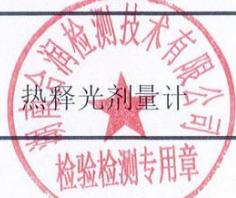
\includegraphics[width=0.85\linewidth]{images/441acd1f9b467295a7d14b65d71c63adcd49ad56a1e73e4627f587c355bcd998.jpg}
\end{figure}


样品名称：

Sample name

报告日期：

Date ofReport

\subsubsection{注意事项}

\subsubsection{CONSIDERATIONS}

1.本报告无检验检测机构“检测报告专用章”无效。

2.本报告无CMA"标志不具备法律证明作用。

3.复制本报告未重新加盖“检测报告专用章”无效。

8.本报告解释权归检验检测单位。

\subsubsection{检测报告}

\subsubsection{REPORTOFTEST}

报告编号：

24HRJLW0038Q03

委托单位：

萍乡市人民医院

ReportNo.

Client

1.本次监测的主要技术依据(Referencedocuments forthe test)：

《职业性外照射个人监测监测规范》（GBZ128—2019）

《电离辐射防护与放射源安全基本标准》（GB18871—2002）

2.本次监测的环境条件(Environment condition forthe test)：

60\%RH

3.本次监测所使用的主要测量设备(Main standardsofmeasurementused inthe test)：

证书号/有效期

溯源机构

Description/Model

Certificate No./Due Date

Traceability Institute

热释光剂量仪/RGD-3D

SC1904019

2024H21-20-

5449245001/2025.9.3

上海市计量测试技术研究院/华东

国家计量测试中心

\begin{figure}[H]
\centering
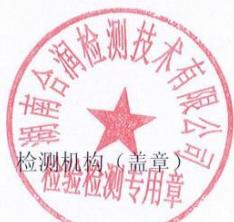
\includegraphics[width=0.85\linewidth]{images/a722b293dfa8e4717f36ef4b4a32469fdb9e34787fd90567e7f19c761b3dc80d.jpg}
\end{figure}


罗素明

\subsubsection{湖南合润检测技术有限公司}

\subsubsection{检测报告}

样品受理编号： 2403W0038


\begin{table}[H]
\centering
\begin{tabular}{|c|c|c|c|}
\hline
检测项目 & 个人剂量监测 & 检测方法 & 热释光检测法 \\
\hline
用人单位 & 萍乡市人民医院 & 委托单位 & 萍乡市人民医院 \\
\hline
检测/评价依据 & GBZ 128-2019职业性外照射个人监测规范 & 检测日期 & 2024年11月4日 \\
\hline
检测室名称 & 个人剂量室 & 检测类别/目的 & 委托/常规监测 \\
\hline
检测仪器名称/型号/编号 & 热释光剂量仪/RGD-3D/SC1904019 & 探测器 & 热释光剂量计(TLD)-片状(圆片)-LiF(Mg,Cu,P) \\
\hline
\end{tabular}
\end{table}


检测结果：

\begin{table}[H]
\centering
\begin{tabular}{|c|c|c|c|c|c|c|c|}
\hline
编号 & 姓名 & 性别 & 职业类别 & 剂量计佩戴起止日期 & 个人剂量当量 (mSv) &  &  \\
\hline
铅衣外( H\_\{p\}(10) ) & 铅衣内( H\_\{p\}(10) ) & 有效剂量( H\_\{p\}(10) ) &  &  &  &  &  \\
\hline
W0038001P & 邹南安 & 男 & 诊断放射学(2A) & 2024/7/1-2024/9/30 &  &  & 0.07 \\
\hline
W0038002P & 巫启恒 & 男 & 诊断放射学(2A) & 2024/7/1-2024/9/30 &  &  & 0.09 \\
\hline
W0038003P & 黎英 & 女 & 诊断放射学(2A) & 2024/7/1-2024/9/30 &  &  & 0.02*\# \\
\hline
W0038004P & 刘锋 & 男 & 诊断放射学(2A) & 2024/7/1-2024/9/30 &  &  & 0.09 \\
\hline
W0038005P & 刘小红 & 女 & 诊断放射学(2A) & 2024/7/1-2024/9/30 &  &  & 0.05 \\
\hline
W0038006P & 李丰章 & 男 & 诊断放射学(2A) & 2024/7/1-2024/9/30 &  &  & 0.02* \\
\hline
W0038007P & 黄元发 & 男 & 诊断放射学(2A) & 2024/7/1-2024/9/30 &  &  & 0.02* \\
\hline
W0038008P & 曾志宏 & 男 & 诊断放射学(2A) & 2024/7/1-2024/9/30 &  &  & 0.02* \\
\hline
W0038009P & 谭华 & 男 & 诊断放射学(2A) & 2024/7/1-2024/9/30 &  &  & 0.02* \\
\hline
W0038010P & 陈萍赣 & 男 & 诊断放射学(2A) & 2024/7/1-2024/9/30 &  &  & 0.02* \\
\hline
W0038011P & 郭欣 & 男 & 诊断放射学(2A) & 2024/7/1-2024/9/30 &  &  & 0.02* \\
\hline
W0038012P & 钟自华 & 男 & 诊断放射学(2A) & 2024/7/1-2024/9/30 &  &  & 0.08 \\
\hline
W0038013P & 陈洋勇 & 男 & 诊断放射学(2A) & 2024/7/1-2024/9/30 &  &  & 0.02* \\
\hline
W0038014P & 刘霞 & 女 & 诊断放射学(2A) & 2024/7/1-2024/9/30 &  &  & 0.02* \\
\hline
W0038015P & 陈亮 & 男 & 诊断放射学(2A) & 2024/7/1-2024/9/30 &  &  & 0.02* \\
\hline
\end{tabular}
\end{table}


检测结果：


\begin{table}[H]
\centering
\begin{tabular}{|c|c|c|c|c|c|c|c|}
\hline
编号 & 姓名 & 性别 & 职业类别 & 剂量计佩戴起止日期 & 个人剂量当量(mSv) &  &  \\
\hline
铅衣外 & 铅衣内 & 有效剂量 &  &  &  &  &  \\
\hline
Hp(10) & Hp(10) & Hp(10) &  &  &  &  &  \\
\hline
W0038016P & 傅志颖 & 女 & 诊断放射学(2A) & 2024/7/1-2024/9/30 &  &  & 0.02* \\
\hline
W0038017P & 李琪 & 男 & 诊断放射学(2A) & 2024/7/1-2024/9/30 &  &  & 0.02* \\
\hline
W0038018P & 周晶 & 女 & 诊断放射学(2A) & 2024/7/1-2024/9/30 &  &  & 0.02* \\
\hline
W0038019P & 肖维国 & 男 & 诊断放射学(2A) & 2024/7/1-2024/9/30 &  &  & 0.02* \\
\hline
W0038020P & 刘天笑 & 女 & 诊断放射学(2A) & 2024/7/1-2024/9/30 &  &  & 0.02* \\
\hline
W0038021P & 王敬朋 & 男 & 诊断放射学(2A) & 2024/7/1-2024/9/30 &  &  & 0.09 \\
\hline
W0038022P & 王爱华 & 女 & 诊断放射学(2A) & 2024/7/1-2024/9/30 &  &  & 0.02* \\
\hline
W0038023P & 崔甜甜 & 女 & 诊断放射学(2A) & 2024/7/1-2024/9/30 &  &  & 0.02* \\
\hline
W0038024P & 杜红 & 女 & 诊断放射学(2A) & 2024/7/1-2024/9/30 &  &  & 0.02* \\
\hline
W0038025P & 文翠 & 女 & 诊断放射学(2A) & 2024/7/1-2024/9/30 &  &  & 0.02* \\
\hline
W0038026P & 易鑫 & 男 & 诊断放射学(2A) & 2024/7/1-2024/9/30 &  &  & 0.02* \\
\hline
W0038027P & 贺曦 & 男 & 诊断放射学(2A) & 2024/7/1-2024/9/30 &  &  & 0.02* \\
\hline
W0038028P & 万红 & 女 & 诊断放射学(2A) & 2024/7/1-2024/9/30 &  &  & 0.02* \\
\hline
W0038029P & 廖林 & 女 & 诊断放射学(2A) & 2024/7/1-2024/9/30 &  &  & 0.05 \\
\hline
W0038030P & 张晓玲 & 女 & 诊断放射学(2A) & 2024/7/1-2024/9/30 &  &  & 0.02* \\
\hline
W0038031P & 黎安琪 & 女 & 诊断放射学(2A) & 2024/7/1-2024/9/30 &  &  & 0.02* \\
\hline
W0038032P & 吴正波 & 男 & 诊断放射学(2A) & 2024/7/1-2024/9/30 &  &  & 0.02* \\
\hline
W0038033P & 王德华 & 男 & 诊断放射学(2A) & 2024/7/1-2024/9/30 &  &  & 0.02* \\
\hline
W0038034P & 吴斌 & 男 & 诊断放射学(2A) & 2024/7/1-2024/9/30 &  &  & 0.02* \\
\hline
W0038035P & 易阳 & 女 & 诊断放射学(2A) & 2024/7/1-2024/9/30 &  &  & 0.09 \\
\hline
W0038036P & 汤裕兵 & 男 & 诊断放射学(2A) & 2024/7/1-2024/9/30 &  &  & 0.02* \\
\hline
W0038037P & 黄瑶 & 女 & 诊断放射学(2A) & 2024/7/1-2024/9/30 &  &  & 0.02* \\
\hline
W0038038P & 雍好琴 & 女 & 诊断放射学(2A) & 2024/7/1-2024/9/30 &  &  & 0.04 \\
\hline
W0038039P & 杨迪 & 女 & 诊断放射学(2A) & 2024/7/1-2024/9/30 &  &  & 0.02* \\
\hline
W0038040P & 王敏 & 女 & 诊断放射学(2A) & 2024/7/1-2024/9/30 &  &  & 0.02* \\
\hline
W0038041P & 杨道益 & 男 & 诊断放射学(2A) & 2024/7/1-2024/9/30 &  &  & 0.02* \\
\hline
W0038042P & 沈雯婷 & 女 & 诊断放射学(2A) & 2024/7/1-2024/9/30 &  &  & 0.02* \\
\hline
W0038043P & 捷继斯 & 男 & 诊断放射学(2A) & 2024/7/1-2024/9/30 &  &  & 0.02* \\
\hline
\end{tabular}
\end{table}


检测结果：


\begin{table}[H]
\centering
\begin{tabular}{|c|c|c|c|c|c|c|c|}
\hline
编号 & 姓名 & 性别 & 职业类别 & 剂量计佩戴起止日期 & 个人剂量当量(mSv) &  &  \\
\hline
铅衣外 & 铅衣内 & 有效剂量 &  &  &  &  &  \\
\hline
Hp(10) & Hp(10) & Hp(10) &  &  &  &  &  \\
\hline
W0038044P & 龙安友 & 男 & 诊断放射学(2A) & 2024/7/1-2024/9/30 &  &  & 0.02* \\
\hline
W0038045P & 周宇煊 & 男 & 诊断放射学(2A) & 2024/7/1-2024/9/30 &  &  & 0.02* \\
\hline
W0038046P & 陈智勇 & 男 & 诊断放射学(2A) & 2024/7/1-2024/9/30 &  &  & 0.07 \\
\hline
W0038047P & 何婷 & 女 & 诊断放射学(2A) & 2024/7/1-2024/9/30 &  &  & 0.04 \\
\hline
W0038048P & 张崇海 & 男 & 诊断放射学(2A) & 2024/7/1-2024/9/30 &  &  & 0.04 \\
\hline
W0038049P & 黄紫娴 & 女 & 诊断放射学(2A) & 2024/7/1-2024/9/30 &  &  & 0.02* \\
\hline
W0038050P & 龙阳天利 & 女 & 诊断放射学(2A) & 2024/7/1-2024/9/30 &  &  & 0.02* \\
\hline
W0038051P & 李健 & 男 & 诊断放射学(2A) & 2024/7/1-2024/9/30 &  &  & 0.02* \\
\hline
W0038052P & 叶作增 & 男 & 诊断放射学(2A) & 2024/7/1-2024/9/30 &  &  & 0.02* \\
\hline
W0038053P & 周礼平 & 男 & 诊断放射学(2A) & 2024/7/1-2024/9/30 &  &  & 0.02* \\
\hline
W0038054P & 黄丽 & 女 & 诊断放射学(2A) & 2024/7/1-2024/9/30 &  &  & 0.02*\# \\
\hline
W0038055P & 靡洪 & 男 & 诊断放射学(2A) & 2024/7/1-2024/9/30 &  &  & 0.05 \\
\hline
W0038056P & 廖晓慧 & 女 & 诊断放射学(2A) & 2024/7/1-2024/9/30 &  &  & 0.02* \\
\hline
W0038057P & 邓莎 & 女 & 诊断放射学(2A) & 2024/7/1-2024/9/30 &  &  & 0.02* \\
\hline
W0038058P & 易江 & 男 & 诊断放射学(2A) & 2024/7/1-2024/9/30 &  &  & 0.02* \\
\hline
W0038059P & 彭向丽 & 女 & 诊断放射学(2A) & 2024/7/1-2024/9/30 &  &  & 0.02* \\
\hline
W0038060P & 唐志武 & 男 & 诊断放射学(2A) & 2024/7/1-2024/9/30 &  &  & 0.07 \\
\hline
W0038061P & 彭其 & - & 诊断放射学(2A) & 2024/7/1-2024/9/30 &  &  & 0.02* \\
\hline
W0038062P & 刘涛 & - & 诊断放射学(2A) & 2024/7/1-2024/9/30 &  &  & 0.09 \\
\hline
W0038063P & 廖延亮 & 男 & 诊断放射学(2A) & 2024/7/1-2024/9/30 &  &  & 0.02*\# \\
\hline
W0038064P & 蔡坤豪 & 男 & 诊断放射学(2A) & 2024/7/1-2024/9/30 &  &  & 0.02* \\
\hline
W0038065P & 欧阳公怒 & 男 & 其他应用(2F) & 2024/7/1-2024/9/30 &  &  & 0.02* \\
\hline
W0038066P & 陈明伟 & 男 & 放射治疗(2D) & 2024/7/1-2024/9/30 &  &  & 0.02* \\
\hline
W0038067P & 黄华堂 & 男 & 放射治疗(2D) & 2024/7/1-2024/9/30 &  &  & 0.02* \\
\hline
W0038068P & 张红宇 & 女 & 放射治疗(2D) & 2024/7/1-2024/9/30 &  &  & 0.06 \\
\hline
W0038069P & 辛焕中 & 男 & 放射治疗(2D) & 2024/7/1-2024/9/30 &  &  & 0.02* \\
\hline
W0038070P & 胡依冰 & 女 & 放射治疗(2D) & 2024/7/1-2024/9/30 &  &  & 0.02* \\
\hline
W0038071P & 刘鲁根 & 男 & 放射治疗(2D) & 2024/7/1-2024/9/30 &  &  & 0.02* \\
\hline
\end{tabular}
\end{table}


检测结果：


\begin{table}[H]
\centering
\begin{tabular}{|c|c|c|c|c|c|c|c|}
\hline
编号 & 姓名 & 性别 & 职业类别 & 剂量计佩戴起止日期 & 个人剂量当量(mSv) &  &  \\
\hline
铅衣外Hp(10) & 铅衣内Hp(10) & 有效剂量Hp(10) &  &  &  &  &  \\
\hline
W0038072P & 乔浩 & 男 & 放射治疗(2D) & 2024/7/1-2024/9/30 &  &  & 0.04 \\
\hline
W0038073P & 黄珍 & 女 & 放射治疗(2D) & 2024/7/1-2024/9/30 &  &  & 0.05 \\
\hline
W0038074P & 李露 & 女 & 放射治疗(2D) & 2024/7/1-2024/9/30 &  &  & 0.02* \\
\hline
W0038075P & 周怡 & 女 & 放射治疗(2D) & 2024/7/1-2024/9/30 &  &  & 0.02* \\
\hline
W0038076K & 李鹏 & 男 & 核医学(2C) & 2024/7/1-2024/9/30 & 0.10 & 0.04 &  \\
\hline
W0038077K & 杨凭飞 & 男 & 核医学(2C) & 2024/7/1-2024/9/30 & 0.05 & 0.02* &  \\
\hline
W0038078K & 文晓琴 & 女 & 核医学(2C) & 2024/7/1-2024/9/30 & 0.05 & 0.02* &  \\
\hline
W0038079K & 黎心四 & 男 & 核医学(2C) & 2024/7/1-2024/9/30 & 0.20 & 0.07 &  \\
\hline
W0038080K & 张西 & 女 & 核医学(2C) & 2024/7/1-2024/9/30 & 0.20 & 0.04 &  \\
\hline
W0038081K & 王健 & 男 & 核医学(2C) & 2024/7/1-2024/9/30 & 0.09 & 0.02* &  \\
\hline
W0038082K & 任妹 & 女 & 核医学(2C) & 2024/7/1-2024/9/30 & 0.07 & 0.02* &  \\
\hline
W0038083K & 周慧 & 女 & 核医学(2C) & 2024/7/1-2024/9/30 & 0.09 & 0.04 &  \\
\hline
W0038084K & 陈娇 & 女 & 核医学(2C) & 2024/7/1-2024/9/30 & 0.08 & 0.06 &  \\
\hline
W0038085K & 许优 & 女 & 核医学(2C) & 2024/7/1-2024/9/30 & 0.11 & 0.08 &  \\
\hline
W0038086K & 董文哲 & 男 & 介入放射学(2E) & 2024/7/1-2024/9/30 & 0.02* & 0.02* &  \\
\hline
W0038087K & 肖江 & 女 & 介入放射学(2E) & 2024/7/1-2024/9/30 & 0.02* & 0.02* &  \\
\hline
W0038088K & 郑磊 & 男 & 介入放射学(2E) & 2024/7/1-2024/9/30 & 0.02* & 0.02* &  \\
\hline
W0038089K & 林婷 & 女 & 介入放射学(2E) & 2024/7/1-2024/9/30 & 0.02* & 0.02* &  \\
\hline
W0038090K & 周春春 & 女 & 介入放射学(2E) & 2024/7/1-2024/9/30 & 0.02* & 0.02* &  \\
\hline
W0038091K & 杨侃 & 男 & 介入放射学(2E) & 2024/7/1-2024/9/30 & 0.02* & 0.02* &  \\
\hline
W0038092K & 易瀚杰 & 男 & 介入放射学(2E) & 2024/7/1-2024/9/30 & 0.02* & 0.02* &  \\
\hline
W0038093K & 刘晨曦 & 女 & 介入放射学(2E) & 2024/7/1-2024/9/30 & 0.02*\# & 0.02* &  \\
\hline
W0038094K & 李苏琴 & 女 & 介入放射学(2E) & 2024/7/1-2024/9/30 & 0.04 & 0.02* &  \\
\hline
W0038095K & 刘建刚 & 男 & 介入放射学(2E) & 2024/7/1-2024/9/30 & 0.02* & 0.02* &  \\
\hline
W0038096K & 刘霞 & 女 & 介入放射学(2E) & 2024/7/1-2024/9/30 & 0.02* & 0.02* &  \\
\hline
W0038097K & 彭治鹏 & 男 & 介入放射学(2E) & 2024/7/1-2024/9/30 & 0.05 & 0.02* &  \\
\hline
W0038098K & 张涵茹 & 女 & 介入放射学(2E) & 2024/7/1-2024/9/30 & 0.02*\# & 0.02* &  \\
\hline
W0038099K & 朱敏 & 女 & 介入放射学(2E) & 2024/7/1-2024/9/30 & 0.12 & 0.02* &  \\
\hline
\end{tabular}
\end{table}


检测结果：


\begin{table}[H]
\centering
\begin{tabular}{|c|c|c|c|c|c|c|c|}
\hline
编号 & 姓名 & 性别 & 职业类别 & 剂量计佩戴起止日期 & 个人剂量当量(mSv) &  &  \\
\hline
铅衣外Hp(10) & 铅衣内Hp(10) & 有效剂量Hp(10) &  &  &  &  &  \\
\hline
W0038100K & 韩涛 & 男 & 介入放射学(2E) & 2024/7/1-2024/9/30 & 1.68 & 0.99 &  \\
\hline
W0038101K & 廖骞 & 男 & 介入放射学(2E) & 2024/7/1-2024/9/30 & 0.02* & 0.02* &  \\
\hline
W0038102K & 蔡恒烈 & 男 & 介入放射学(2E) & 2024/7/1-2024/9/30 & 0.02* & 0.02* &  \\
\hline
W0038103K & 王奕 & 男 & 介入放射学(2E) & 2024/7/1-2024/9/30 & 0.02* & 0.02* &  \\
\hline
W0038104K & 张志强 & 男 & 介入放射学(2E) & 2024/7/1-2024/9/30 & 0.87 & 0.09 &  \\
\hline
W0038105K & 崔钢 & 男 & 介入放射学(2E) & 2024/7/1-2024/9/30 & 6.21 & 0.25 &  \\
\hline
W0038106K & 严兵 & 男 & 介入放射学(2E) & 2024/7/1-2024/9/30 & 1.47\# & 0.23\# &  \\
\hline
W0038107K & 龚敏 & 男 & 介入放射学(2E) & 2024/7/1-2024/9/30 & 0.02* & 0.02* &  \\
\hline
W0038108K & 韩明 & 男 & 介入放射学(2E) & 2024/7/1-2024/9/30 & 0.02* & 0.02* &  \\
\hline
W0038109K & 邱萍 & 男 & 介入放射学(2E) & 2024/7/1-2024/9/30 & 0.02* & 0.02* &  \\
\hline
W0038110K & 贺娇 & 女 & 介入放射学(2E) & 2024/7/1-2024/9/30 & 0.02*\# & 0.02* &  \\
\hline
W0038111K & 付云辉 & 男 & 介入放射学(2E) & 2024/7/1-2024/9/30 & 0.02* & 0.02* &  \\
\hline
W0038112K & 吴朝 & 男 & 介入放射学(2E) & 2024/7/1-2024/9/30 & 0.02* & 0.02* &  \\
\hline
W0038113K & 郑旺 & 男 & 介入放射学(2E) & 2024/7/1-2024/9/30 & 0.02* & 0.02* &  \\
\hline
W0038114K & 兰前鑫 & 男 & 介入放射学(2E) & 2024/7/1-2024/9/30 & 0.02*\# & 0.02* &  \\
\hline
W0038115K & 朱勇美 & 女 & 介入放射学(2E) & 2024/7/1-2024/9/30 & 0.02* & 0.02* &  \\
\hline
W0038116K & 黄文军 & 男 & 介入放射学(2E) & 2024/7/1-2024/9/30 & 0.45 & 0.02* &  \\
\hline
W0038117K & 周国忠 & 男 & 介入放射学(2E) & 2024/7/1-2024/9/30 & 0.15 & 0.02* &  \\
\hline
W0038118K & 罗勤 & 男 & 介入放射学(2E) & 2024/7/1-2024/9/30 & 1.99 & 0.02*\# &  \\
\hline
W0038119K & 姚常 & 男 & 介入放射学(2E) & 2024/7/1-2024/9/30 & 2.88 & 0.02* &  \\
\hline
W0038120K & 彭阳 & 男 & 介入放射学(2E) & 2024/7/1-2024/9/30 & 1.26\# & 0.02* &  \\
\hline
W0038121K & 刘兴龙 & 男 & 介入放射学(2E) & 2024/7/1-2024/9/30 & 0.02* & 0.02* &  \\
\hline
W0038122K & 周吕桢 & 男 & 介入放射学(2E) & 2024/7/1-2024/9/30 & 1.26\# & 0.02* &  \\
\hline
W0038123K & 陈小根 & - & 介入放射学(2E) & 2024/7/1-2024/9/30 & 0.02* & 0.02* &  \\
\hline
W0038124K & 闫博宇 & 男 & 介入放射学(2E) & 2024/7/1-2024/9/30 & 0.13 & 0.02* &  \\
\hline
W0038125K & 张学洪 & 男 & 介入放射学(2E) & 2024/7/1-2024/9/30 & 0.08\# & 0.02* &  \\
\hline
W0038126K & 张雨虹 & 男 & 介入放射学(2E) & 2024/7/1-2024/9/30 & 1.75\# & 0.02* &  \\
\hline
W0038127K & 曾广忠 & 男 & 介入放射学(2E) & 2024/7/1-2024/9/30 & 3.31 & 0.02*\# &  \\
\hline
\end{tabular}
\end{table}


检测结果：
共7页第6页

\begin{table}[H]
\centering
\begin{tabular}{|c|c|c|c|c|c|c|c|}
\hline
编号 & 姓名 & 性别 & 职业类别 & 剂量计佩戴起止日期 & 个人剂量当量(mSv) &  &  \\
\hline
铅衣外 & 铅衣内 & 有效剂量 &  &  &  &  &  \\
\hline
Hp(10) & Hp(10) & Hp(10) &  &  &  &  &  \\
\hline
W0038128K & 邱明涛 & 男 & 介入放射学(2E) & 2024/7/1-2024/9/30 & 1.93 & 0.02*\# &  \\
\hline
W0038129K & 邓海明 & 男 & 介入放射学(2E) & 2024/7/1-2024/9/30 & 0.02* & 0.02* &  \\
\hline
W0038130K & 邱建 & 男 & 介入放射学(2E) & 2024/7/1-2024/9/30 & 1.75\# & 0.02* &  \\
\hline
W0038131K & 李晨 & 男 & 介入放射学(2E) & 2024/7/1-2024/9/30 & 1.75\# & 0.02* &  \\
\hline
W0038132K & 赖丹 & 男 & 介入放射学(2E) & 2024/7/1-2024/9/30 & 0.02* & 0.02* &  \\
\hline
W0038133K & 毛云飞 & 男 & 介入放射学(2E) & 2024/7/1-2024/9/30 & 1.02 & 0.02* &  \\
\hline
W0038134K & 刘帅 & 男 & 介入放射学(2E) & 2024/7/1-2024/9/30 & 0.02* & 0.02* &  \\
\hline
W0038135K & 胡斌 & 男 & 介入放射学(2E) & 2024/7/1-2024/9/30 & 0.02* & 0.02* &  \\
\hline
W0038136K & 彭成福 & 男 & 介入放射学(2E) & 2024/7/1-2024/9/30 & 0.10 & 0.02*\# &  \\
\hline
W0038137K & 李洛 & 男 & 介入放射学(2E) & 2024/7/1-2024/9/30 & 0.72 & 0.04 &  \\
\hline
W0038138K & 朱飞 & 男 & 介入放射学(2E) & 2024/7/1-2024/9/30 & 1.29 & 1.28 &  \\
\hline
W0038139K & 丁绍纯 & 男 & 介入放射学(2E) & 2024/7/1-2024/9/30 & 0.02* & 0.02* &  \\
\hline
W0038140K & 王稻 & 男 & 介入放射学(2E) & 2024/7/1-2024/9/30 & 0.02* & 0.02* &  \\
\hline
W0038141K & 刘灏灏 & 男 & 介入放射学(2E) & 2024/7/1-2024/9/30 & 0.02* & 0.02* &  \\
\hline
W0038142K & 孙芬芬 & 女 & 介入放射学(2E) & 2024/7/1-2024/9/30 & 0.02* & 0.02* &  \\
\hline
W0038143K & 王俊东 & 男 & 介入放射学(2E) & 2024/7/1-2024/9/30 & 0.02* & 0.02* &  \\
\hline
W0038144K & 廖鹏 & 男 & 介入放射学(2E) & 2024/7/1-2024/9/30 & 0.02* & 0.02* &  \\
\hline
W0038145K & 贺小张 & 男 & 介入放射学(2E) & 2024/7/1-2024/9/30 & 0.02* & 0.02* &  \\
\hline
W0038146K & 许绍林 & 男 & 介入放射学(2E) & 2024/7/1-2024/9/30 & 0.02* & 0.02* &  \\
\hline
W0038147K & 余凯龙 & 男 & 介入放射学(2E) & 2024/7/1-2024/9/30 & 0.02* & 0.02* &  \\
\hline
W0038148K & 胡芯源 & 男 & 介入放射学(2E) & 2024/7/1-2024/9/30 & 0.35 & 0.02* &  \\
\hline
W0038149K & 王长庚 & 男 & 介入放射学(2E) & 2024/7/1-2024/9/30 & 0.02* & 0.02* &  \\
\hline
W0038150K & 杨德猛 & 男 & 介入放射学(2E) & 2024/7/1-2024/9/30 & 1.26 & 0.02* &  \\
\hline
W0038151K & 姜一帆 & 男 & 介入放射学(2E) & 2024/7/1-2024/9/30 & 0.54\# & 0.02*\# &  \\
\hline
W0038152K & 胡小辉 & 男 & 介入放射学(2E) & 2024/7/1-2024/9/30 & 0.46 & 0.02* &  \\
\hline
W0038153K & 曹世超 & 男 & 介入放射学(2E) & 2024/7/1-2024/9/30 & 1.12 & 0.02* &  \\
\hline
W0038154K & 徐辉 & 男 & 介入放射学(2E) & 2024/7/1-2024/9/30 & 0.02* & 0.02* &  \\
\hline
W0038155K & 漆招 & 男 & 介入放射学(2E) & 2024/7/1-2024/9/30 & 0.02* & 0.02* &  \\
\hline
\end{tabular}
\end{table}


检测结果：


\begin{table}[H]
\centering
\begin{tabular}{|c|c|c|c|c|c|c|c|}
\hline
编号 & 姓名 & 性别 & 职业类别 & 剂量计佩戴起止日期 & 个人剂量当量(mSv) &  &  \\
\hline
铅衣外 & 铅衣内 & 有效剂量 &  &  &  &  &  \\
\hline
 &  &  &  &  & Hp(10) & Hp(10) & Hp(10) \\
\hline
W0038156K & 巫志国 & 男 & 介入放射学(2E) & 2024/7/1-2024/9/30 & 0.02* & 0.02* &  \\
\hline
W0038157K & 柳毅 & 男 & 介入放射学(2E) & 2024/7/1-2024/9/30 & 0.02* & 0.02* &  \\
\hline
W0038158K & 沈婕 & 女 & 介入放射学(2E) & 2024/7/1-2024/9/30 & 0.02* & 0.02* &  \\
\hline
W0038159K & 刘可可 & 女 & 介入放射学(2E) & 2024/7/1-2024/9/30 & 0.02* & 0.02* &  \\
\hline
W0038 & 本底 & - & - & 2024/7/1-2024/9/30 &  &  & 0.38 \\
\hline
\end{tabular}
\end{table}


\begin{figure}[H]
\centering
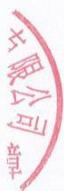
\includegraphics[width=0.85\linewidth]{images/663f0ddd27253644129b259899d58a81fe2f08dfedaa71b93e9aa8256b49a95c.jpg}
\end{figure}


\section{后装治疗机房原有检测报告}

\begin{figure}[H]
\centering

\includegraphics[width=0.85\linewidth]{images/11ddc1681d2e99fc841a02379aac8b154bbb327ab825bb860ebd8e60e4234363.jpg}
\end{figure}


湖南合润检测技术有限公司

HUNAN HERUN TESTING TECHNOLOGY CO.,LTD

\begin{figure}[H]
\centering

\includegraphics[width=0.85\linewidth]{images/c64bdcaa38327ac2b2393c84f7a42f019d41b882e9197d181153a97498b81084.jpg}
\end{figure}


211803102214

检测报告

报告编号：24HR128WB48

后装治疗设备防护性能检测检测项目： 及工作场所防护检测

萍乡市人民医院

萍乡市武功山中大道8号

委托检测/状态检测

\begin{figure}[H]
\centering
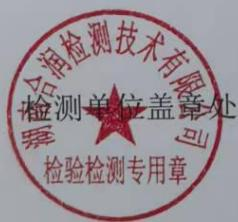
\includegraphics[width=0.85\linewidth]{images/f8156b8cb2b492f1cebca543e724d17638a6907bd9c483124d30d58e69a8b337.jpg}
\end{figure}


报告日期：2024年07月01日

检测单位：湖南合润检测技术有限公司

邮编：410221

电话：0731-85058578

传真：0731-85058578

\subsubsection{注意事项}

1、本报告无检验检测机构“检测报告专用章"无效；
2、本报告无“CMA”标志不具备法律证明作用；
3、复制本报告未重新加盖“检测报告专用章”无效；
4、本报告无报告签发人（授权签字人）签名无效；
5、本报告涂改无效；
6、对本检验报告若有异议，应于收到报告之日起十五日内向检验单位提出，逾期不予受理；
7、本报告仅对所委托检测的样品负责；
8、本报告解释权归检验检测单位；
9、本报告一式两份，一份给委托单位，一份为本单位存档。

声明：湖南合润检测技术有限公司为独立的第三方检测机构，公司规定全体员工必须遵守以下声明要求：

\begin{enumerate}
\item 严格遵守相关的法律、法规，依照公司质量管理体系开展检验检测活动，为客户提供科学、公正、准确满意的服务；
\item 本公司及公司全体人员不得与其从事的检验检测活动以及出具的数据和结果存在利益关系；绝不参与任何有损于检验检测判断的独立性和诚信度的活动：绝不参与和检验检测项目或者类似的竞争性项目有关系的产品设计、研制、生产供应、安装、使用或者维护活动，保证出具的数据准确可靠、公正客观：
\item 本公司及全体员工对其在检验检测活动中所知悉的国家秘密、商业秘密和技术秘密负有保密义务，对客户的产品、技术、数据等相关信息严格保密，经客户同意，保证不提供给其他单位或个人。
\end{enumerate}

湖南合润检测技术有限公司

报告编号：24HR128WB48

湖南合润检测技术有限公司
检测报告

\begin{table}[H]
\centering
\begin{tabular}{|c|c|c|c|}
\hline
设备名称 & 高剂量率γ射线遥控后装治疗机 & 设备型号 & XHDR18B \\
\hline
生产厂家 & 山东新华医疗器械股份有限公司 & 设备序列号 & H058 \\
\hline
检测项目 & 后装治疗设备防护性能及工作场所防护检测 & 检测地点 & 放疗楼一楼后装机房 \\
\hline
检测时间 & 2024年06月16日 & 额定参数 & 192Ir \\
\hline
检测条件 & 温度:23.3℃ & 气压:99.72kPa &  \\
\hline
检测/评价依据 & 1、《后装γ源近距离治疗质量控制检测规范》(WS 262-2017)2、《放射治疗放射防护要求》(GBZ 121-2020) &  &  \\
\hline
仪器编号 & 仪器名称 & 仪器型号 & 检定/校准有效期至 \\
\hline
HRJC/YQ15 & 放疗剂量仪 & MAX 4000Plus + HDR1000Plus & 2025年01月04日 \\
\hline
HRJC/YQ29 & 空盒气压表 & DYM3 & 2024年12月12日 \\
\hline
HRJC/YQ31 & 水银温度计 & 棒式 & 2024年12月12日 \\
\hline
HRJC/YQ41 & 辐射检测仪 & AT1123 & 2025年04月25日 \\
\hline
检测结论: 本次检测结果符合标准《后装γ源近距离治疗质量控制检测规范》(WS 262-2017)和《放射治疗放射防护要求》(GBZ 121-2020)中的相关要求。 (本页以下空白) &  &  &  \\
\hline
\end{tabular}
\end{table}


湖南合润检测技术有限公司

报告编号：24HR128WB48

性能检测结果

\begin{table}[H]
\centering
\begin{tabular}{|c|c|c|c|c|c|}
\hline
序号 & 检测项目 & 判定标准 & 检测结果 & 合格 (是/否) & 备注 \\
\hline
1 & 源活度 & ±5\% & 1.29\% & 是 & 最大响应点：84.5cm 显示源活度：3.7246mCi 实测源活度：3.6670mCi \\
\hline
2 & 源传输到位精度 & ±1mm & -0.1mm & 是 & 85cm \\
\hline
3 & 放射源累计定位误差 & ±1mm & -0.2mm & 是 & 步进2.5mm \\
\hline
4 & 源驻留时间误差 & ±0.5s & -0.05s & 是 & 60s \\
\hline
5 & 贮源器表面泄漏辐射所致周围剂量当量率 & ≤50μSv/h & 0.77μSv/h & 是 & 距设备外表面5cm处 \\
\hline
≤5μSv/h & 0.29μSv/h & 是 & 距设备外表面100cm处 &  &  \\
\hline
\end{tabular}
\end{table}


（本页以下空白）

湖南合润检测技术有限公司

报告编号：24HR128WB48

\subsubsection{防护检测结果}

\begin{table}[H]
\centering
\begin{tabular}{|c|c|c|c|c|c|}
\hline
序号 & 检测位置 & 检测结果 (μSv/h) & 标准限值 (μSv/h) & 判定结果 & 备注 \\
\hline
1 & 操作位（操作室） & <MDL & ≤2.5 & 合格 & 192Ir; 3.6670Ci; 出源 \\
\hline
2 & 机房防护门外（走廊） & <MDL & ≤2.5 & 合格 & 192Ir; 3.6670Ci; 出源 \\
\hline
3 & 机房防护门上门缝外30cm处（走廊） & <MDL & ≤2.5 & 合格 & 192Ir; 3.6670Ci; 出源 \\
\hline
4 & 机房防护门下门缝外30cm处（走廊） & <MDL & ≤2.5 & 合格 & 192Ir; 3.6670Ci; 出源 \\
\hline
5 & 机房防护门左门缝外30cm处（走廊） & <MDL & ≤2.5 & 合格 & 192Ir; 3.6670Ci; 出源 \\
\hline
6 & 机房防护门右门缝外30cm处（走廊） & <MDL & ≤2.5 & 合格 & 192Ir; 3.6670Ci; 出源 \\
\hline
7 & 机房西墙外30cm处（操作室） & <MDL & ≤2.5 & 合格 & 192Ir; 3.6670Ci; 出源 \\
\hline
8 & 机房西墙外30cm处（操作室） & <MDL & ≤2.5 & 合格 & 192Ir; 3.6670Ci; 出源 \\
\hline
9 & 机房西墙外30cm处 (走廊) & <MDL & ≤2.5 & 合格 & 192Ir; 3.6670Ci; 出源 \\
\hline
10 & 机房北墙外30cm处 (处置室) & <MDL & ≤2.5 & 合格 & 192Ir; 3.6670Ci; 出源 \\
\hline
11 & 机房北墙外30cm处 (处置室) & <MDL & ≤2.5 & 合格 & 192Ir; 3.6670Ci; 出源 \\
\hline
12 & 机房北墙外30cm处 (处置室) & <MDL & ≤2.5 & 合格 & 192Ir; 3.6670Ci; 出源 \\
\hline
注： 1. 表内检测数据均已扣除本底值。 2. 待检设备未出束状态下本底平均值：0.16μSv/h。 3. MDL=0.08。 &  &  &  &  &  \\
\hline
\end{tabular}
\end{table}


\begin{figure}[H]
\centering
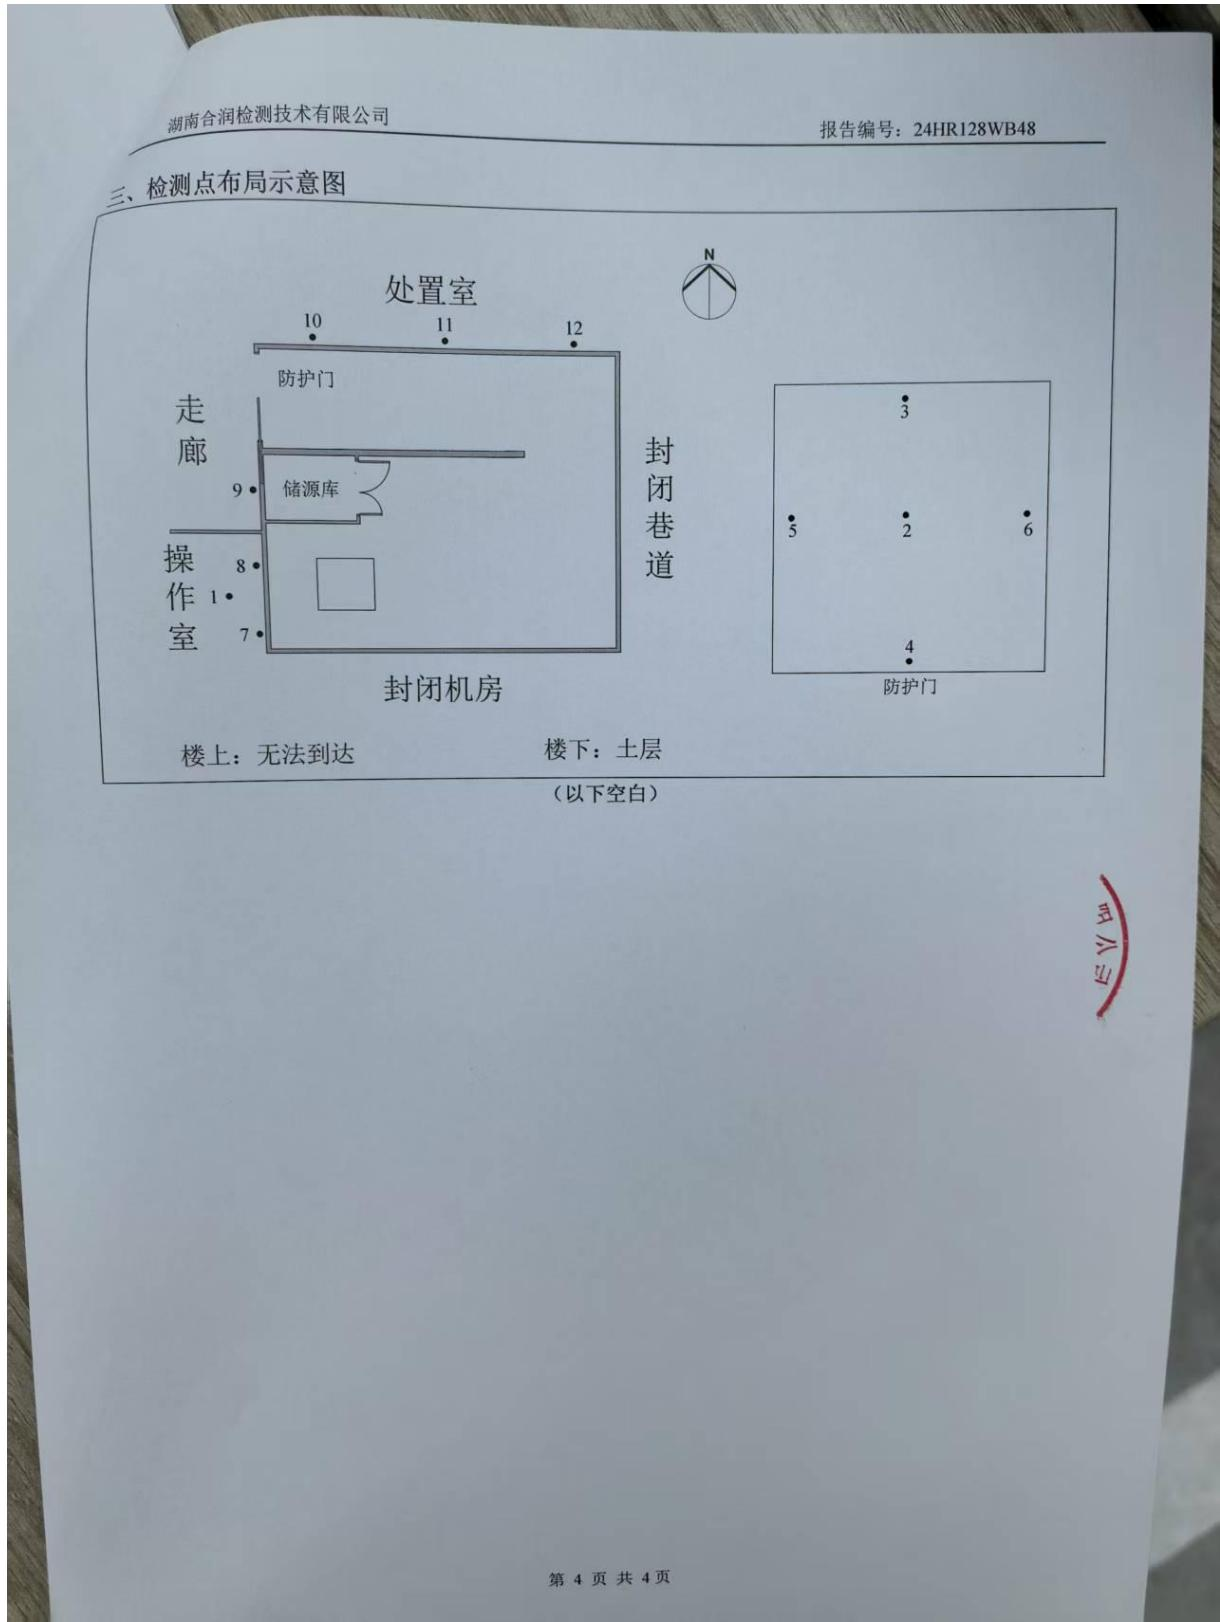
\includegraphics[width=0.85\linewidth]{images/681f101817242c57988c416220a8989977f4da0738fd8f5c7afd89f287fc3dfd.jpg}
\end{figure}


\section{本项目评审意见}

\subsubsection{关于《萍乡市人民医院后装治疗机机房改建项目放射性职业病危害预评价报告书》的评审意见}

根据《中华人民共和国职业病防治法》《放射诊疗管理规定》《放射诊疗建设项目卫生审查管理规定》等法律法规、规章的要求，江西辐射剂量检测院有限公司（以下简称“评价单位”）组织有关专家于2025年8月21日中午在南昌市对评价单位编制的《萍乡市人民医院后装治疗机机房改建项目放射性职业病危害预评价报告书》（报告编号：YP250420）（以下简称《预评价报告书》）进行了评审。专家组听取了萍乡市人民医院对建设项目情况的介绍和评价单位对《预评价报告书》的介绍，经过讨论和评议，形成评审意见如下：

一、《预评价报告书》依据的法律法规、规章和标准准确，评价内容较全面，评价方法适当，对建设项目辐射源项和职业病危害因素分析较全面，对拟采取的防护设施、防护措施评价适当，结论正确、建议基本可行。

\subsubsection{二、建议：}

\begin{enumerate}
\item 完善放射工作人员的个人剂量估算；
\item 完善项目利旧情况说明；
\item 落实专家组提出的其他意见。
\end{enumerate}

\subsubsection{三、结论：}

专家组建议《预评价报告书》修改后通过，《预评价报告书》按专家组意见修改并经组长签字确认后依程序上报。

专家组成员：

2025年8月2日

\section{专家评审意见及修改情况}

\begin{table}[H]
\centering
\begin{tabular}{|c|c|c|c|c|c|}
\hline
序号 & 评审意见 & 送审稿页码 & 报批稿对应页码 & 修改说明 &  \\
\hline
1 & 完善放射工作人员的个人剂量估算 & 48 & 48 & 已完善放射工作人员的个人剂量估算 &  \\
\hline
2 & 完善项目利旧情况说明 & 21 & 21 & 完善项目利旧情况说明 &  \\
\hline
4 & 落实专家组提出的其他意见。 & 核实人员配备 & 12 & 12 & 已核实人员配备情况 \\
\hline
完善本项目路径情况 & 20 & 20 & 已完善本项目路径情况 &  &  \\
\hline
其他文本格式错误 & 全文 & 全文 & 已对全文文本格式进行更新 &  &  \\
\hline
\end{tabular}
\end{table}
